\setcounter{dang}{0}
\section{THỂ TÍCH}
\subsection{Trọng tâm kiến thức}
\begin{tomtat}
\subsubsection*{Công thức tính thể tích}
\begin{boxdn}
	Phần không gian được giới hạn bởi hình chóp, hình chóp cụt đều, hình lăng trụ, hình hộp tương ứng được gọi là khối chóp, khối chóp cụt đều, khối lăng trụ, khối hộp. Đỉnh, mặt, cạnh, đường cao của các khối đó lần lượt là đỉnh, cạnh, đường cao của hình chóp, hình chóp cụt đều, hình lăng trụ, hình hộp tương ứng
	\begin{itemize}
	\item Thể tích của khối chóp có diện tích đáy $S$ và chiều cao $h$ là 
	$$V=\dfrac{1}{3}\cdot h\cdot .$$
	\item Thể tích của khối chóp cụt đều có diện tích đáy lớn $S$, diện tích đáy bé $S'$ và chiều cao $h$ là 
	$$V\dfrac{1}{3}\cdot h\cdot (S+S'+\sqrt{S\cdot S'}).$$
	\item Thể tích của khối lăng trụ có diện tích đáy $S$ và chiều cao $h$ là 
	$$V=h\cdot S.$$
	\end{itemize}
\end{boxdn}
\begin{minipage}[t]{0.33\textwidth}
	\begin{tikzpicture}[scale=.8,font=\footnotesize,line join = round, line cap = round, >= stealth]
	%\draw[opacity=0.3] (0,0) grid (6,6);
	\def\x{4} \def\y{2} \def\z{3.5}
	\def\g{-120}
	\coordinate (A) at (0,0);
	\coordinate (E) at ($(A)+(0:\x)$);
	\coordinate (B) at ($(A)+(-60:1.3)$);
	\coordinate (C) at ($(B)+(-30:1)$);
	\coordinate (D) at ($(C)+(20:2)$);
	\coordinate (H) at ($(A)+(-30:1.5)$);
	\coordinate (S) at ($(H)+(90:\z)$);
	\draw (S)--(A)--(B)--(C)--(D)--(E)--(S)--(D)
	(B)--(S)--(C)
	;
	\draw[dashed] (A)--(E) (S)--(H) 
	;
	\foreach \p/\g in {S/100,A/180,B/-90,C/-70,D/-20,E/0,H/-90} \draw[fill] (\p) circle(.5pt)
	node [shift={(\g:.3)}] {$\p$}
	;
	\draw (1.15,1)node{$h$}
	;
	\end{tikzpicture}
\end{minipage}
\begin{minipage}[t]{0.33\textwidth}
	\begin{tikzpicture}[scale=.8,font=\footnotesize,line join = round, line cap = round, >= stealth]
	%\draw[opacity=0.3] (0,0) grid (6,6);
	\def\x{4} \def\y{2} \def\z{3.5}
	\def\g{-120}
	\coordinate (A) at (0,0);
	\coordinate (B) at ($(A)+(0:\x)$);
	\coordinate (D) at ($(A)+(40:\y)$);
	\coordinate (C) at ($(B)+(D)-(A)$);
	\coordinate (H) at ($(A)!1/2!(C)$);
	\coordinate (S) at ($(H)+(90:\z)$);
	\coordinate (A') at ($(S)!0.4!(A)$);
	\coordinate (B') at ($(S)!0.4!(B)$);
	\coordinate (C') at ($(S)!0.4!(C)$);
	\coordinate (D') at ($(S)!0.4!(D)$);
	\coordinate (H') at ($(S)!0.4!(H)$);
	\draw (2.5,2)node{$h$}
	;
	\draw (A')--(B')--(C')--(D')--
	(A')--(A)--(B)--(C)--(C')
	(B)--(B') (A')--(C') (B')--(D')
	;
	\draw[dashed] (A)--(D)--(C)--(A) (B)--(D)--(D')
	(H)--(H')
	;
	\foreach \p/\g in {A/-100,B/-90,C/0,D/180,H/-90,A'/180,B'/-30,C'/0,D'/180,H'/90} \draw[fill] (\p) circle(.5pt)
	node [shift={(\g:.3)}] {$\p$}
	;
	\end{tikzpicture}
\end{minipage}
\begin{minipage}[t]{0.33\textwidth}
	\begin{tikzpicture}[scale=.8,font=\footnotesize,line join = round, line cap = round, >= stealth]
	%\draw[opacity=0.3] (0,0) grid (6,6);
	\def\x{4} \def\y{2} \def\z{3.5}
	\def\g{-120}
	\coordinate (A) at (0,0);
	\coordinate (B) at ($(A)+(0:\x)$);
	\coordinate (C) at ($(A)+(40:\y)$);
	\coordinate (H) at ($(A)+(10:2.3)$);
	\coordinate (B') at ($(H)+(90:\z)$);
	\coordinate (A') at ($(A)+(B')-(B)$);
	\coordinate (C') at ($(A')+(C)-(A)$);
	\draw (A')--(B')--(C')--cycle
	(A')--(A)--(B)--(B')
	;
	\draw[dashed] (C')--(C)--(A) (C)--(B) (B')--(H)
	;
	\foreach \p/\g in {A/-100,B/-80,C/30,H/-90,A'/180,B'/80,C'/90} \draw[fill] (\p) circle(.5pt)
	node [shift={(\g:.3)}] {$\p$};
	\draw (2,2)node{$h$}
	;
	\end{tikzpicture}
\end{minipage}
\begin{nx}
	\begin{itemize}
	\item Thể tích khối tứ diện bằng một phần ba tích của chiều cao từ một đỉnh và diện tích mặt đối diện với đỉnh đó.
	\item Thể tích của khối hộp bằng tích của một mặt và chiều cao của khối hộp ứng với mặt đó.
	\end{itemize}
\end{nx}
\end{tomtat}
%%%%%%%%%%%%
\subsection{Các dạng bài tập}
\begin{dang}{Thể tích khối chóp đều, chóp cụt đều}
\end{dang}
\subsubsection{Ví dụ minh hoạ}
\begin{vd}%[2H1Y3-2]
	Cho khối chóp đều $S.ABC$ có cạnh đáy bằng $a$. Tính thể tích khối chóp $S.ABC$ biết cạnh bên bằng $2a$.
	\loigiai{
	\immini{
	Gọi $M$ là trung điểm của $BC$. Gọi $G$ là trọng tâm tam giác $ABC$, do $S.ABC$ là hình chóp đều nên $SG\perp \left( ABC\right)$. \\
	Vì $\triangle ABC$ đều cạnh $a$ nên $AM=\dfrac{a\sqrt{3}}{2}\Rightarrow S_{\triangle ABC}=\dfrac{a^2\sqrt{3}}{4}$.\\
	Ta có $AG=\dfrac{2}{3}AM=\dfrac{2}{3}\cdot\dfrac{a\sqrt{3}}{2}=\dfrac{a\sqrt{3}}{3}$.\\
	Do $SG\perp \left( ABC\right)$ nên $\triangle SAG$ vuông tại $G$\\
	$\Rightarrow SG=\sqrt{SA^2-AG^2}=\sqrt{4a^2-\dfrac{a^2}{3}}=\dfrac{a\sqrt{11}}{\sqrt{3}}$. \\
	Vậy $V=\dfrac{1}{3}\cdot S_{\triangle ABC}\cdot SG=\dfrac{1}{3}\cdot \dfrac{a^2\sqrt{3}}{4}\cdot \dfrac{a\sqrt{11}}{\sqrt{3}}=\dfrac{a^3\sqrt{11}}{12}$.}{
	\begin{tikzpicture}[scale=1, line join = round, line cap = round]
	\tikzset{label style/.style={font=\footnotesize}}
	\tkzDefPoints{0/0/A,5/0/C,1.5/-2/B}
	\tkzCentroid(A,B,C)\tkzGetPoint{G}
	\coordinate (S) at ($(G)+(0,4)$);
	\coordinate (M) at ($(B)!0.5!(C)$);
	\tkzMarkRightAngles[size=0.2](S,G,A)
	\tkzMarkSegments[mark=|](M,B M,C)
	\tkzDrawPolygon(S,A,B,C)
	\tkzDrawSegments(S,B S,M)
	\tkzDrawSegments[dashed](A,C S,G A,M)
	\tkzDrawPoints[fill=black](A,B,C,S,G,M)
	\tkzLabelPoints[above](S)
	\tkzLabelPoints[below](B,M,G)
	\tkzLabelPoints[left](A)
	\tkzLabelPoints[right](C)
	\end{tikzpicture}}
	}
\end{vd}
\begin{vd}%[2H1K3-2]
	Cho hình chóp tứ giác đều $S.ABCD$, cạnh đáy $AB=2a\sqrt{3}$, mặt bên tạo với đáy góc $60^\circ$. Tính thể tích thể tích của khối chóp $S.ABCD$.
	\loigiai{
	\immini{
	Gọi $O$ là tâm hình vuông $ABCD$ và $M$ là trung điểm $CD$, khi đó \\
	$\left\{\begin{aligned}&CD \perp SM \\&CD \perp OM \end{aligned}\right.\Rightarrow CD \perp (SOM)$\\
	Suy ra $\widehat{\left( \left(SCD\right),\left(ABCD\right)\right)}=\widehat{\left(SM,OM \right)}=\widehat{SMO}=60^\circ$. \\
	Vì $S.ABCD$ là hình chóp đều nên $SO \perp (ABCD)$, do đó $\triangle SOM$ vuông tại $O$.\\
	$\Rightarrow SO=OM\cdot\tan 60^\circ=a\sqrt{3}\cdot \sqrt{3}=3a$.\\ 
	Vậy $V_{S.ABCD}=\dfrac{1}{3}Sh=\dfrac{1}{3}\left(2a\sqrt{3}\right)^2\cdot 3a=12a^3$.
	}{
	\begin{tikzpicture}[scale=0.55, line join = round, line cap = round]
	\tikzset{label style/.style={font=\footnotesize}}
	\tkzDefPoints{0/0/B,7/0/C,3/3/A}
	\coordinate (D) at ($(A)+(C)-(B)$);
	\tkzInterLL(A,C)(B,D) \tkzGetPoint{O}
	\coordinate (S) at ($(O)+(0,7)$);
	\coordinate (M) at ($(C)!0.5!(D)$);
	\tkzMarkRightAngles[size=0.4](S,O,M)
	\tkzMarkSegments[mark=|](M,D M,C)
	\tkzDrawPolygon(S,D,C,B)
	\tkzDrawSegments(S,C S,M)
	\tkzDrawSegments[dashed](A,S A,D A,B A,C B,D S,O O,M)
	\tkzDrawPoints[fill=black](D,C,A,B,O,S,M)
	\tkzLabelPoints[above](S)
	\tkzLabelPoints[left](A,B)
	\tkzLabelPoints[right](D,C,M)
	\tkzLabelPoints[below](O)
	\end{tikzpicture}
	}
	}
\end{vd}
\begin{vd}%[2H1B3-2]
	Cho hình chóp tứ giác đều $S.ABCD$ có cạnh bên bằng $a$, góc giữa cạnh bên hợp với mặt đáy bằng $60^\circ.$ Tính theo $a$ thể tích khối chóp $S.ABCD$.
	\loigiai{
	\immini{
	Gọi $O$ là giao $AC$ và $BD$. Vì $S.ABCD$ chóp đều nên $SO\perp (ABCD)$.\\
	Góc hợp bởi các cạnh bên và mặt đáy bằng $60^\circ$ nên $$\widehat{SAO}=\widehat{SBO}=\widehat{SCO}=\widehat{SDO}=60^\circ. $$
	Mặt khác $SA=SB=SC=SD=a\Rightarrow$ $\triangle SAO$ là nửa tam giác đều và $\triangle SBD$ đều. \\
	Do đó $SO=SA\cdot \sin {{60}^{o}}=\dfrac{a\sqrt{3}}{2}$;
	$BD=SD=a\Rightarrow AB=\dfrac{a\sqrt{2}}{2}.$\\
	Vậy thể tích khối chóp là $V_{S.ABCD}=\dfrac{1}{3}\cdot S_{ABCD}\cdot SO=\dfrac{a^3\sqrt{3}}{12}.$ }{
	\begin{tikzpicture}[scale=0.6, line join = round, line cap = round]
	\tikzset{label style/.style={font=\footnotesize}}
	\tkzDefPoints{0/0/B,7/0/C,3/3/A}
	\coordinate (D) at ($(A)+(C)-(B)$);
	\tkzInterLL(A,C)(B,D) \tkzGetPoint{O}
	\coordinate (S) at ($(O)+(0,7)$);
	\tkzMarkRightAngles[size=0.4](S,O,C S,O,B)
	\tkzDrawPolygon(S,D,C,B)
	\tkzDrawSegments(S,C)
	\tkzDrawSegments[dashed](A,S A,D A,B A,C B,D S,O)
	\tkzDrawPoints[fill=black](D,C,A,B,O,S)
	\tkzLabelPoints[above](S)
	\tkzLabelPoints[left](A,B)
	\tkzLabelPoints[right](D,C)
	\tkzLabelPoints[above right](O)
	\end{tikzpicture}}	
	}
\end{vd}
\begin{vd}%[2H1K3-2]
	Cho hình chóp tứ giác đều $S.ABCD$ có đáy là hình vuông tâm $O$ cạnh bằng $2a$. Gọi $I$ là trung điểm của $SO$. Biết khoảng cách từ $I$ đến mặt phẳng $(SBC)$ bằng $\dfrac{a\sqrt{5}}{5}$. Tính thể tích của khối chóp $S.ABCD$.
	\loigiai{	
	\immini{
	Gọi $M$ là trung điểm của $BC$\\
	Ta có $\left\{\begin{aligned}&BC \perp SM \\&BC \perp OM \end{aligned}\right.\Rightarrow BC\perp (SOM)$.\\
	Ta có $OM=\dfrac{CD}{2}=\dfrac{2a}{2}=a$.\\
	Gọi $H$, $K$ lần lượt là hình chiếu của $O$, $I$ trên $SM$.\\
	Ta có $\left\{\begin{aligned}&IK\perp SM \\&IK \perp BC\,(\text{vì }BC\perp (SOM) \end{aligned}\right.$ \\
	$\Rightarrow\mathrm{d}\left(I,(SBC)\right)=IK=\dfrac{a\sqrt{5}}{5}$.\\
	$IK$ là đường trung bình $\triangle SOH$\\
	$\Rightarrow OH=2IK=\dfrac{2a\sqrt{5}}{5}.$\\
	}{
	\begin{tikzpicture}[scale=0.6, line join = round, line cap = round]
	\tikzset{label style/.style={font=\footnotesize}}
	\tkzInit[xmin=-1,xmax=10,ymin=-1,ymax=9.5]
	\tkzClip
	%\tkzAxeXY
	\tkzDefPoints{0/0/D,6/0/C,3/3/A}
	\coordinate (B) at ($(A)+(C)-(D)$);
	\tkzInterLL(A,C)(B,D) \tkzGetPoint{O}
	\coordinate (S) at ($(O)+(0,6.5)$);
	\coordinate (I) at ($(S)!0.5!(O)$);
	\coordinate (M) at ($(B)!0.5!(C)$);
	\tkzDefPointBy[projection = onto S--M](O)\tkzGetPoint{H}
	\tkzDefPointBy[projection = onto S--M](I)\tkzGetPoint{K}
	\tkzMarkRightAngles[size=0.3](S,O,M I,K,M O,H,M)
	\tkzMarkSegments[mark=|](M,B M,C)
	\tkzMarkSegments[mark=||](I,S I,O)
	\tkzDrawPolygon(S,D,C,B)
	\tkzDrawSegments(S,C S,M)
	\tkzDrawSegments[dashed](A,S A,D A,B A,C B,D S,O I,K O,H O,M)
	\tkzDrawPoints[fill=black](D,C,A,B,O,S,I,H,K,M)
	\tkzLabelPoints[above](S)
	\tkzLabelPoints[below](O)
	\tkzLabelPoints[below right](C)
	\tkzLabelPoints[left](D,I)
	\tkzLabelPoints[above left](A)
	\tkzLabelPoints[right](B,H,K,M)
	\end{tikzpicture}}
	\noindent 	Xét tam giác $SOM$ vuông tại $O$, đường cao $OH$, ta có:
	$\dfrac{1}{SO^2}+\dfrac{1}{OM^2}=\dfrac{1}{OH^2}\Rightarrow SO=2a$.\\
	Khi đó $V_{S.ABCD}=\dfrac{1}{3}SO\cdot S_{ABCD}=\dfrac{8a^3}{3}$.
	}
\end{vd}
\begin{vd}%[1C8B6-3]
	Cho khối chóp cụt tam giác đều $ABC.A'B'C'$ có chiều cao bằng $3a$, $AB=4a$, $A'B'=a$. Tính thể tích của khối chóp cụt đều $ABC.A'B'C'$.
	\loigiai
	{\immini{Diện tích tam giác đều $A B C$ là
	$$S_1=\dfrac{1}{2}AB\cdot AC\cdot\sin \widehat{BAC}=\dfrac{1}{2}\cdot 4a\cdot 4a\cdot\sin 60^{\circ}=4\sqrt{3}a^2.$$
	Diện tích tam giác đều $A'B'C'$ là
	$$S_2=\dfrac{1}{2}A'B'\cdot A'C'\cdot\sin \widehat{B'A'C'}=\dfrac{1}{2}\cdot a\cdot a\cdot\sin 60^{\circ}=\dfrac{\sqrt{3}a^2}{4}.$$
	Thể tích khối chóp cụt đều $ABC.A'B'C'$ là
	$$V=\dfrac{1}{3}\cdot 3a\cdot\left(4\sqrt{3}a^2+\sqrt{4\sqrt{3}a^2\cdot\dfrac{\sqrt{3}a^2}{4}}+\dfrac{\sqrt{3}a^2}{4}\right)
	=\dfrac{21\sqrt{3}a^3}{4}.$$}{
	\begin{tikzpicture}[scale=1, font=\footnotesize, line join=round, line cap=round,>=stealth]
	\def \k{0.6};
	\path (0,0)coordinate (A) (3.5,0) coordinate (C) (2.5,-1) coordinate (B) ($(B)!0.5!(C)$) coordinate (M) ($(A)!2/3!(M)$) coordinate (O) (0,3) coordinate (h) ($(O)+(h)$) coordinate (S);
	\foreach \p in {A,B,C}{\path ($(\p)!\k!(S)$) coordinate (\p');}
	\draw (A')--(A)--(B)--(C)--(C')--cycle (B')--(C') (A')--(B')--(B);
	\draw[dashed] (A)--(C);
	\foreach \p/\g in {A/150,B/-60,C/30, A'/150, B'/-30, C'/30} \fill[black] (\p) circle(1pt)+(\g:0.3) node{$\p$};
	\end{tikzpicture}}
	}
\end{vd}
%-----------------------------
\subsubsection{Bài tập áp dụng}
\begin{bt}%[2H1Y3-2]
	Cho hình chóp tam giác đều $S.ABC$ có $AB=a$, cạnh bên $SA=\dfrac{a\sqrt{6}}{3}$. Tính thể tích của khối chóp $S.ABC$.
	\loigiai{
%	\immini{
	Gọi $G$ là trọng tâm tam giác $ABC$ suy ra $SG\perp \left( ABC\right)$.\\
	Gọi $M$ là trung điểm của $BC$ ta có $AM=\dfrac{a\sqrt{3}}{2}$.\\
	Khi đó $AG=\dfrac{2}{3}AM=\dfrac{2}{3}\cdot\dfrac{a\sqrt{3}}{2}=\dfrac{a\sqrt{3}}{3}$.\\
	Lại có $SG=\sqrt{SA^2-AG^2}=\sqrt{\dfrac{2a^2}{3}-\dfrac{a^2}{3}}=\dfrac{a\sqrt{3}}{3}$\\
	Vậy $V_{S.ABC}=\dfrac{1}{3}\cdot SG\cdot S_{ABC}=\dfrac{1}{3}\cdot \dfrac{a\sqrt{3}}{3}\cdot\dfrac{a^2\sqrt{3}}{4}=\dfrac{a^3}{12}$.\\
%	}{
	\begin{center}
	\begin{tikzpicture}[scale=1, line join = round, line cap = round]
	\tikzset{label style/.style={font=\footnotesize}}
	\tkzDefPoints{0/0/A,5/0/C,1.5/-1.5/B}
	\tkzCentroid(A,B,C)\tkzGetPoint{G}
	\coordinate (S) at ($(G)+(0,4)$);
	\coordinate (M) at ($(B)!0.5!(C)$);
	\tkzMarkRightAngles[size=0.2](S,G,A)
	\tkzMarkSegments[mark=|](M,B M,C)
	\tkzDrawPolygon(S,A,B,C)
	\tkzDrawSegments(S,B S,M)
	\tkzDrawSegments[dashed](A,C S,G A,M)
	\tkzDrawPoints[fill=black](A,B,C,S,G,M)
	\tkzLabelPoints[above](S)
	\tkzLabelPoints[below](B,M,G)
	\tkzLabelPoints[left](A)
	\tkzLabelPoints[right](C)
	\end{tikzpicture}
	\end{center}
%	}
	}
\end{bt}
\begin{bt}%[2H1K3-2]
	Cho hình chóp tứ giác đều $S.ABCD$ có cạnh đáy bằng $a$ và mặt bên tạo với đáy một góc $45^\circ$. Tính thể tích khối chóp $S.ABCD$.
	\loigiai{
	\immini{
	Gọi $O$ là hình chiếu vuông góc của $A$ trên $(ABCD)$, $M$ là trung điểm của $BC$.\\
	Ta có
	$\widehat{SMO}=45^\circ\Rightarrow SO=OM=\dfrac{a}{2}$.\\
	Do đó $V_{S.ABCD}=\dfrac{a^3}{6}$.
	}{
	\begin{tikzpicture}[scale=0.5, line join = round, line cap = round]
	\tikzset{label style/.style={font=\footnotesize}}
	\tkzDefPoints{0/0/B,9/0/C,3.5/2.5/A}
	\coordinate (D) at ($(A)+(C)-(B)$);
	\tkzInterLL(A,C)(B,D) \tkzGetPoint{O}
	\coordinate (S) at ($(O)+(0,6.5)$);
	\coordinate (M) at ($(C)!0.5!(D)$);
	\tkzMarkRightAngles[size=0.4](S,O,M)
	\tkzMarkSegments[mark=|](M,D M,C)
	\tkzDrawPolygon(S,D,C,B)
	\tkzDrawSegments(S,C S,M)
	\tkzDrawSegments[dashed](A,S A,D A,B A,C B,D S,O O,M)
	\tkzDrawPoints[fill=black](D,C,A,B,O,S,M)
	\tkzLabelPoints[above](S)
	\tkzLabelPoints[left](A,B)
	\tkzLabelPoints[right](D,C,M)
	\tkzLabelPoints[below](O)
	\end{tikzpicture}
	}
	}
\end{bt}
\begin{bt}%[2H1B3-2]
	Cho hình chóp tam giác đều $S.ABC$ có cạnh đáy bằng $a$, cạnh bên tạo với đáy một góc $45^\circ$. Tính thể tích khối chóp $S.ABC$.
	\loigiai{
	\immini{
	Gọi $G$ là trọng tâm $\triangle ABC$.\\
	Góc tạo bởi cạnh bên và mặt đáy $\widehat{SBG}=45^\circ$.\\
	$G$ là trọng tâm $\triangle ABC\Rightarrow BG=\dfrac{a\sqrt{3}}{3}$.\\
	Do đó $AG=BG\cdot \tan \widehat{ABG}=\dfrac{a\sqrt{3}}{3}\cdot \tan 45^\circ=\dfrac{a\sqrt{3}}{3}$.\\
	Vậy thể tích là\\
	$V=\dfrac{1}{3}\cdot S_{\triangle ABC}\cdot AG=\dfrac{1}{3}\cdot \dfrac{1}{2}\cdot a\cdot \dfrac{a\sqrt{3}}{2}\cdot \dfrac{a\sqrt{3}}{3}=\dfrac{a^3}{12}. $
	}{
	\begin{tikzpicture}[scale=.7, line join = round, line cap = round]
	\tikzset{label style/.style={font=\footnotesize}}
	\tkzDefPoints{0/0/A,7/0/C,2/-3/B}
	\tkzCentroid(B,C,A) \tkzGetPoint{G}
	\coordinate (S) at ($(G)+(0,5)$);
	\tkzMarkRightAngles[size=0.2](S,G,B)
	\tkzDrawPolygon(S,A,B,C)
	\tkzDrawSegments(S,B)
	\tkzDrawSegments[dashed](A,C S,G A,G)
	\tkzDrawPoints[fill=black](A,B,C,D,G)
	\tkzLabelPoints[above](S)
	\tkzLabelPoints[below](B)
	\tkzLabelPoints[left](A)
	\tkzLabelPoints[right](G,C)
	\end{tikzpicture}
	}
	}
\end{bt}
\begin{bt}%[2H1K3-2]
	Cho hình chóp đều $S.ABC$ có cạnh đáy bằng $a$, khoảng cách giữa cạnh bên $SA$ và cạnh đáy $BC$ bằng $\dfrac{3a}{4}$. Tính thể tích khối chóp $S.ABC$.
	\loigiai{
	Gọi $I$ là trung điểm của $BC$. Kẻ đường cao $IK$ của tam giác $SAI$. Gọi $O$ là trọng tâm tam giác $ABC$, đặt $SO=h$. Ta có
	\immini{
	$S_{\triangle ABC}=\dfrac{1}{2}a^2\sin 60^\circ=\dfrac{a^2\sqrt{3}}{4}$;\\ $AI=\sqrt{a^2-\left(\dfrac{a}{2}\right)^2}=\dfrac{a\sqrt{3}}{2}\Rightarrow AO=\dfrac{a\sqrt{3}}{3}$.\\
	$SA=\sqrt{SO^2+AO^2}=\sqrt{h^2+\left( \dfrac{a\sqrt{3}}{3}\right)^2}=\sqrt{h^2+\dfrac{a^2}{3}}$.\\
	Lại có $SO\cdot AI=KI\cdot SA\Leftrightarrow h\cdot \dfrac{a\sqrt{3}}{2}=\dfrac{3a}{4}\sqrt{h^2+\dfrac{a^2}{3}}\Leftrightarrow h=a$.\\
	Thể tích khối chóp $S.ABCD$ là\\ $V=\dfrac{1}{3}\cdot S_{\triangle ABC}\cdot SO=\dfrac{1}{3}\cdot\dfrac{a^2\sqrt{3}}{4}\cdot a=\dfrac{a^2\sqrt{3}}{12}$.
	}{
	\begin{tikzpicture}[scale=0.75, line join = round, line cap = round]
	\tikzset{label style/.style={font=\footnotesize}}
	\tkzDefPoints{0/0/A,6/0/C,1.5/-2/B}
	\tkzCentroid(A,B,C)\tkzGetPoint{O}
	\coordinate (S) at ($(O)+(0,4.5)$);
	\coordinate (I) at ($(B)!0.5!(C)$);
	\tkzDefPointBy[projection = onto A--S](I)\tkzGetPoint{K}
	\tkzMarkRightAngles[size=0.2](S,O,A I,K,S S,I,C)
	\tkzMarkSegments[mark=|](I,B I,C)
	\tkzDrawPolygon(S,A,B,C)
	\tkzDrawSegments(S,B S,I)
	\tkzDrawSegments[dashed](A,C S,O I,K A,I)
	\tkzDrawPoints[fill=black](A,B,C,S,O,I,K)
	\tkzLabelPoints[above](S)
	\tkzLabelPoints[below](B,I,O)
	\tkzLabelPoints[left](A,K)
	\tkzLabelPoints[right](C)
	\end{tikzpicture}
	}
	}
\end{bt}
\begin{bt}%[1K7KQ-2]
	\immini{Một sọt đựng đồ có dạng hình chóp cụt đều. Đáy và miệng sọt là các hình vuông tương ứng có cạnh bằng $60$ cm, $30$ cm, cạnh bên của sọt dài $50$ cm. Tính thể tích của sọt. }{
	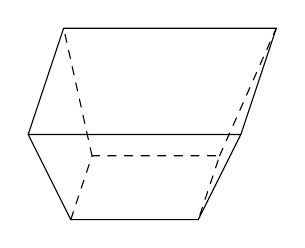
\begin{tikzpicture}[scale=0.6, font=\footnotesize, line join=round, line cap=round, >=stealth]
	\def\k{0.45}
	\path 
	(1*\k,3*\k) coordinate (A) 
	(7*\k,3*\k) coordinate (B)
	(6*\k,0) coordinate (C)
	(0,0) coordinate (D)
	(-1/3*\k,9*\k) coordinate (A')
	(9*\k+2*\k/3,9*\k) coordinate (B')
	(8*\k,4*\k) coordinate (C')
	(-2*\k,4*\k) coordinate (D')
	; 
	\draw (C)--(D)--(D')--(C')--cycle (C')--(B')--(A')--(D');
	\draw[dashed] (D)--(A)--(B)--(C) (B)--(B') (A)--(A');
	\end{tikzpicture}	
	}
	\loigiai{ 
	Diện tích đáy là $S=60^2=3600$ (cm$^2$).\\
	Diện tích miệng sọt là $S'=30^2=900$ (cm$^2$).\\	
	Chiều cao của hình chóp cụt đều là $h=\sqrt{50^2 -\left( 15\sqrt{2} \right)^2}= 5\sqrt{82}$ (cm). \\
	Thể tích của sọt là $V=\dfrac{1}{3} \cdot h \left(S+S'+\sqrt{S \cdot S'}\right)=10500 \sqrt{82}$ (cm$^3$).
	}
\end{bt}
%%=======================================
\begin{dang}{Thể tích khối chóp có cạnh bên vuông góc với mặt đáy}
\end{dang}
\subsubsection{Ví dụ minh hoạ}
\begin{vd}%[2H1Y3-2]
	Cho hình chóp $S.ABC$ có đáy $ABC$ là tam giác đều cạnh $a$. Cạnh $SA$ vuông góc với mặt đáy $(ABC)$ và $SA=a\sqrt{3}$. Tính thể tích khối chóp $S.ABC$.
	\loigiai{
	\immini{
	Ta có $S_{ABC}=\dfrac{a^2\sqrt{3}}{4}\Rightarrow V_{S.ABC}=\dfrac{1}{3}\cdot SA\cdot S_{ABC}=\dfrac{a^3}{4}$}{
	\begin{tikzpicture}[scale=.4, line join = round, line cap = round]
	\tikzset{label style/.style={font=\footnotesize}}
	\tkzDefPoints{0/0/A,7/0/C,3/-3/B}
	\coordinate (S) at ($(A)+(0,5)$);
	\tkzMarkRightAngles[size=0.4](S,A,C S,A,B)
	\tkzMarkSegments[mark=|](A,B B,C C,A)
	\tkzDrawPolygon(S,A,B,C)
	\tkzDrawSegments(S,B)
	\tkzDrawSegments[dashed](A,C)
	\tkzDrawPoints[fill=black](A,B,C,S)
	\tkzLabelPoints[above](S)
	\tkzLabelPoints[below](B)
	\tkzLabelPoints[left](A)
	\tkzLabelPoints[right](C)
	\end{tikzpicture}
	}	
	}
\end{vd}
\begin{vd}%[1C8B6-2]
	\immini{Tính thể tích của khối chóp $S.ABCD$. Biết đáy $ABCD$ là hình vuông cạnh $a$, $SA \perp (ABCD)$, góc giữa đường thẳng $SB$ và mặt phẳng $(ABCD)$ bằng $60^{\circ}$.}{
	\begin{tikzpicture}[scale=0.9, font=\footnotesize, line join=round, line cap=round,>=stealth]
	\path (0,0)coordinate (B) (3,0) coordinate (C) (4.5,1) coordinate (D) ($(B)+(D)-(C)$) coordinate (A) (0,2.5) coordinate (h) ($(A)+(h)$) coordinate (S);
	\draw (S)--(B)--(C)--(D)--cycle (S)--(C);
	\draw[dashed] (S)--(A)--(B) (A)--(D);
	\foreach \p/\g in {A/150,B/240,C/-60, D/0, S/90} \fill[black] (\p) circle(1pt)+(\g:0.3) node{$\p$};
	\draw pic[draw,"$60^\circ$", angle eccentricity=1.5, angle radius=0.7cm]{angle=A--B--S};
	\end{tikzpicture}}
	\loigiai
	{Do $SA \perp (ABCD)$ và $BA$ chứa trong $(ABCD)$ nên $SA \perp AB$, suy ra $S A=A B \cdot \tan \widehat{SBA}$.\\
	Vì $SA \perp (ABCD)$ nên góc giữa đường thẳng $SB$ và mặt phẳng $(ABCD)$ bằng $\widehat{SBA}$. Suy ra $\widehat{SBA}=60^{\circ}$.\\
	Từ đó, ta có $SA=a\cdot\tan 60^{\circ}=a\sqrt{3}$. Mặt khác, do diện tích hình vuông $ABCD$ là $S_{ABCD}=a^2$ nên thể tích của khối chóp $S.ABCD$ là
	$$V_{S.ABCD}=\dfrac{1}{3}S_{ABCD}\cdot SA=\dfrac{1}{3}\cdot a^2\cdot a\sqrt{3}=\dfrac{a^3\sqrt{3}}{3}.$$
	}
\end{vd}
\begin{vd}%[2H1B3-2]
	Cho hình chóp $S.ABCD$ có đáy là hình vuông cạnh $a$, cạnh bên $SA$ vuông góc với đáy, cạnh bên $SC$ tạo với đáy một góc $60^\circ$. Tính thể tích khối chóp $S.ABCD$. 
	\loigiai{
	\immini{
	Ta có $SA\perp (ABCD)$ nên
	$\widehat{(SC,(ABCD))}=\widehat{SCA}=60^\circ$.\\
	Vì $ABCD$ là hình vuông cạnh $a$ nên $AC=a\sqrt{2}.$\\
	Tam giác $SAC$ vuông tại $A$ nên\\
	$\tan \widehat{SCA}=\dfrac{SA}{AC}\Rightarrow SA=a\sqrt{2}\cdot\tan 60^\circ=a\sqrt{6}$.\\
	Vậy thể tích khối chóp $S.ABCD$ là\\
	$V=\dfrac{1}{3}\cdot SA\cdot S_{ABCD}=\dfrac{1}{3}\cdot a\sqrt{6}\cdot a^2=\dfrac{a^3\sqrt{6}}{3}$.
	}{
	\begin{tikzpicture}[scale=0.4, line join = round, line cap = round]
	\tikzset{label style/.style={font=\footnotesize}}
	\tkzInit[xmin=-1,xmax=11,ymin=-1,ymax=11]
	\tkzClip
	%\tkzAxeXY
	\tkzDefPoints{0/0/D,7/0/C,3/3/A}
	\coordinate (B) at ($(A)+(C)-(D)$);
	\coordinate (S) at ($(A)+(0,7)$);
	\tkzMarkRightAngles[size=0.4](S,A,D S,A,B)
	\tkzMarkAngles[size=1.4cm](S,C,A)
	\tkzLabelAngles[pos=2.3,rotate=0](A,C,S){\tiny $60^\circ$}
	\tkzMarkRightAngles[size=0.4](A,B,C B,C,D C,D,A)
	\tkzMarkSegments[mark=|](D,C C,B)
	\tkzDrawPolygon(S,B,C,D)
	\tkzDrawSegments(S,C)
	\tkzDrawSegments[dashed](A,S A,B A,D A,C)
	\tkzDrawPoints[fill=black](D,C,A,B,S)
	\tkzLabelPoints[above](S)
	\tkzLabelPoints[left](A,D)
	\tkzLabelPoints[right](B,C)
	\end{tikzpicture}	
	}	
	}
\end{vd}
\begin{vd}%[2H1K3-2]
	Cho hình chóp $S.ABC$ có $SA$ vuông góc với mặt phẳng đáy, tam giác $SBC$ đều cạnh $a$, góc giữa mặt phẳng $(SBC)$ và mặt phẳng đáy là $30^\circ$. Tính thể tích của khối chóp $S.ABC$.
	\loigiai{
	\immini{
	Gọi $M$ là trung điểm của $BC$, $\triangle SBC$ đều $\Rightarrow SM\perp BC.$\\
	Mà $SA\perp \left(ABC\right)\Rightarrow SA\perp BC$ và $SM\perp BC$, suy ra $BC\perp \left(SAM\right).$\\
	Ta có $\left\{ \begin{aligned}
	& \left(SAM \right)\cap \left(SBC\right)=SM \\ 
	& \left(SAM \right)\cap \left(ABC\right)=AM 
	\end{aligned} \right.$\\
	$\Rightarrow \widehat{\left(\left(SBC\right),\left(ABC\right) \right)}=\widehat{\left(SM,AM\right)}=\widehat{SMA}$.\\
	Xét $\triangle SAM$ vuông tại $A$, có $\sin \widehat{SMA}=\dfrac{SA}{SM}$\\
	$\Rightarrow SA=\sin 30^\circ\cdot \dfrac{a\sqrt{3}}{2}=\dfrac{a\sqrt{3}}{4}.$\\
	Và $\cos \widehat{SMA}=\dfrac{AM}{SM}\Rightarrow AM=\cos 30^\circ\cdot\dfrac{a\sqrt{3}}{2}=\dfrac{3a}{4}.$\\
	$\Rightarrow S_{ABC}=\dfrac{1}{2}AM\cdot BC=\dfrac{3a^2}{8}\Rightarrow V_{S.ABC}=\dfrac{1}{3}SA\cdot S_{ABC}=\dfrac{a^3\sqrt{3}}{32}.$}{
	\begin{tikzpicture}[scale=.6, line join = round, line cap = round]
	\tikzset{label style/.style={font=\footnotesize}}
	\tkzDefPoints{0/0/A,7/0/C,3/-3/B}
	\coordinate (S) at ($(A)+(0,6)$);
	\tkzMarkRightAngles[size=0.4](S,A,C S,A,B)
	\coordinate (M) at ($(C)!0.5!(B)$);
	\tkzMarkAngles[size=1cm](S,M,A)
	\tkzLabelAngles[pos=1.3,rotate=0](A,M,S){\tiny $30^\circ$}
	\tkzMarkRightAngles[size=0.4](S,M,C)
	\tkzMarkSegments[mark=|](M,B M,C)
	\tkzDrawPolygon(S,A,B,C)
	\tkzDrawSegments(S,B S,M)
	\tkzDrawSegments[dashed](A,C A,M)
	\tkzDrawPoints[fill=black](A,B,C,S)
	\tkzLabelPoints[above](S)
	\tkzLabelPoints[below right](B,M)
	\tkzLabelPoints[left](A)
	\tkzLabelPoints[right](C)
	\end{tikzpicture}}
	}
\end{vd}
\begin{vd}%[2H1K3-2]
	Cho hình chóp $S.ABCD$ có đáy $ABCD$ là hình vuông cạnh $a$ và cạnh bên $SA$ vuông góc với mặt đáy. Gọi $E$ là trung điểm của cạnh $CD$. Biết khoảng cách từ $A$ đến mặt phẳng $\left( SBE \right)$ bằng $\dfrac{2a}{3}$, tính thể tích khối chóp $S.ABCD$ theo $a$.
	\loigiai{
	\immini{
	Kẻ $AK\perp BE$ tại $K$, $AH\perp SK$ tại $H$.\\
	Ta có $BE\perp (SAK)$ nên $(SAK)\perp (SBE)$, do đó\\
	$AH=\mathrm{d}\left( A,\left( SBE \right) \right)=\dfrac{2a}{3}$,
	$BE=\sqrt{B{{C}^{2}}+C{{E}^{2}}}=\dfrac{a\sqrt{5}}{2}$.\\
	Mà $\triangle BCE\backsim \triangle AKB\Rightarrow \dfrac{BC}{AK}=\dfrac{BE}{AB}$\\
	$\Rightarrow AK=\dfrac{BC\cdot AB}{BE}=\dfrac{2a\sqrt{5}}{5}$.\\
	Nên $\dfrac{1}{AH^2}=\dfrac{1}{AK^2}+\dfrac{1}{SA^2}\Rightarrow SA^2=\dfrac{AK^2\cdot AH^2}{AK^2-AH^2}=a^2$\\
	$\Rightarrow SA=a$.\\
	Vậy $V_{S.ABCD}=\dfrac{1}{3}SA\cdot AB\cdot BC=\dfrac{a^3}{3}$}{
	\begin{tikzpicture}[scale=0.5, line join = round, line cap = round]
	\tikzset{label style/.style={font=\footnotesize}}
	\tkzDefPoints{0/0/B,7/0/C,1.5/3/A}
	\coordinate (D) at ($(A)+(C)-(B)$);
	\coordinate (S) at ($(A)+(0,6.5)$);
	\coordinate (E) at ($(C)!0.5!(D)$);
	\coordinate (K) at ($(B)!0.45!(E)$);
	\coordinate (H) at ($(S)!0.5!(K)$);
	\tkzMarkRightAngles[size=0.4](S,A,D S,A,B A,K,B A,H,K)
	\tkzMarkRightAngles[size=0.3](A,D,C D,C,B C,B,A)
	\tkzMarkSegments[mark=|](C,E E,D)
	\tkzDrawPolygon(S,D,C,B)
	\tkzDrawSegments(S,C S,E)
	\tkzDrawSegments[dashed](A,S A,B A,D B,E A,K S,K A,H A,C)
	\tkzDrawPoints[fill=black](D,C,A,B,S,E,K,H)
	\tkzLabelPoints[above](S)
	\tkzLabelPoints[below](K)
	\tkzLabelPoints[left](A,B)
	\tkzLabelPoints[right](D,C,E,H)
	\end{tikzpicture}}
	}
\end{vd}
%--------------------------------
\subsubsection{Bài tập áp dụng}
\begin{bt}%[1K7BQ-1]
	Cho khối tứ diện $OABC$ có $OA$, $OB$, $OC$ đôi một vuông góc với nhau và $OA=a$, $OB=b$, $OC=c$. Tính thể tích của khối tứ diện.
	\loigiai{
	\immini{Tam giác vuông $OBC$ có diện tích là $S_{OBC}=\dfrac{1}{2}bc$.\\
	$OA\perp (OBC)$ nên tứ diện $OABC$ có chiều cao ứng với đỉnh $A$ bằng $OA$.\\
	Vậy thể tích của khối tứ diện là $V_{OABC}=\dfrac{1}{3}OA\cdot S_{OBC}=\dfrac{1}{6}abc$.}{\begin{tikzpicture}[scale=0.85,font=\footnotesize,line join = round, line cap = round, >= stealth]
	%\draw[opacity=0.3] (0,0) grid (6,6);
	\def\x{4} \def\y{2} \def\z{3.5}
	\def\g{-120}
	\coordinate (O) at (0,2);
	\coordinate (C) at ($(O)+(0:\x)$);
	\coordinate (B) at ($(O)+(-60:\y)$);
	\coordinate (A) at ($(O)+(90:\z)$);
	\draw (A)--(B)--(C)--(A)--(O)--(B)
	;
	\draw[dashed] (O)--(C)
	;
	\foreach \p/\g in {A/90,B/-80,C/30,O/180} \draw[fill] (\p) circle(.5pt)
	node [shift={(\g:.3)}] {$\p$};
	\draw (-0.3,4)node{$a$} (0.3,1) node{$b$} (2,2.3)node{$c$};
	;
	\end{tikzpicture}}
	}
\end{bt}
\begin{bt}%[2H1Y3-2]
	Cho hình chóp tứ giác $S.ABCD$ có đáy $ABCD$ là hình vuông cạnh $a$, $SA=2a$ vuông góc với mặt đáy. Tính thể tích của khối chóp $S.ABCD$.	
	\loigiai{
	\immini{
	Ta có $SA\perp (ABCD)$\\
	$\Rightarrow$ Hình chóp $S.ABCD$ có đường cao $SA=2a$ và diện tích đáy $S_{ABCD}=a^2$.\\
	Vậy $V_{S.ABCD}=\dfrac{1}{3}\cdot S_{ABCD}\cdot SA=\dfrac{1}{3}\cdot a^2\cdot 2a=\dfrac{2a^3}{3}$.}{
	\begin{tikzpicture}[scale=0.4, line join = round, line cap = round]
	\tikzset{label style/.style={font=\footnotesize}}
	\tkzDefPoints{0/0/D,7/0/C,3/3/A}
	\coordinate (B) at ($(A)+(C)-(D)$);
	\coordinate (S) at ($(A)+(0,6)$);
	\tkzMarkRightAngles[size=0.4](S,A,D S,A,B)
	\tkzMarkRightAngles[size=0.4](A,B,C B,C,D C,D,A)
	\tkzMarkSegments[mark=|](C,D B,C)
	\tkzDrawPolygon(S,B,C,D)
	\tkzDrawSegments(S,C)
	\tkzDrawSegments[dashed](A,S A,B A,D)
	\tkzDrawPoints[fill=black](D,C,A,B,S)
	\tkzLabelPoints[above](S)
	\tkzLabelPoints[left](A,D)
	\tkzLabelPoints[right](B,C)
	\end{tikzpicture}
	}
	}
\end{bt}
\begin{bt}%[2H1B3-2]
	Cho hình chóp $S.ABC$ có đáy là hình tam giác vuông cân tại $B$ và $SA$ vuông với $(ABC)$. Biết $AC=3a\sqrt{2}$ và góc giữa cạnh bên $SB$ và $(ABC)$ bằng $45^\circ$. Tính thể tích của khối chóp $S.ABC$.
	\loigiai{	
	\immini{
	Ta có $2AB^2=AC^2\Leftrightarrow 2AB^2=\left(3a\sqrt{2}\right)^2\Leftrightarrow AB=3a$.\\
	Tam giác $SAB$ vuông cân tại $A$ nên $SA=SB=3a$.\\
	Thể tích của khối chóp $S.ABC$ là\\
	$V=\dfrac{1}{3}\cdot SA\cdot S_{ABC}=\dfrac{1}{3}\cdot 3a\cdot\dfrac{1}{2}(3a)^2= \dfrac{9a^3}{2}$.
	}{
	\begin{tikzpicture}[scale=.4, line join = round, line cap = round]
	\tikzset{label style/.style={font=\footnotesize}}
	\tkzDefPoints{0/0/A,7/0/C,3/-3/B}
	\coordinate (S) at ($(A)+(0,5)$);
	\tkzMarkRightAngles[size=0.4](S,A,C S,A,B)
	\tkzMarkAngles[size=1.6cm](S,B,A)
	\tkzLabelAngles[pos=2.3,rotate=0](A,B,S){\tiny $45^\circ$}
	\tkzMarkRightAngles[size=0.4](A,B,C)
	\tkzMarkSegments[mark=|](B,A B,C)
	\tkzDrawPolygon(S,A,B,C)
	\tkzDrawSegments(S,B)
	\tkzDrawSegments[dashed](A,C)
	\tkzDrawPoints[fill=black](A,B,C,S)
	\tkzLabelPoints[above](S)
	\tkzLabelPoints[below](B)
	\tkzLabelPoints[left](A)
	\tkzLabelPoints[right](C)
	\end{tikzpicture}
	}
	}
\end{bt}
\begin{bt}%[2H1K3-2]
	Cho hình chóp $S.ABC$ có đáy $ABC$ là tam giác đều cạnh $a$, $SA$ vuông góc với đáy $ABC$; góc giữa $2$ mặt phẳng $\left(SBC\right)$ và $\left(ABC\right)$ bằng $30^\circ $. Tính thể tích khối chóp $S.ABC$
	\loigiai{
	\immini{
	Gọi $M$ là trung điểm của $BC$.\\
	Ta có $\left\{ \begin{aligned}
	& BC\perp AM \\ 
	& BC\perp SA 
	\end{aligned} \right.$\\
	$\Rightarrow BC\perp \left(SAM\right)\Rightarrow \widehat{\left(\left( SBC \right),\left( ABC \right) \right)}=\widehat{SMA}={30^\circ}$.\\
	Ta có $AM=\dfrac{a\sqrt{3}}{2}\Rightarrow SA=\dfrac{AM}{\sqrt{3}}=\dfrac{a}{2}$.\\
	Mà $S_{ABC}=\dfrac{a^2\sqrt{3}}{4}$.\\
	$\Rightarrow V_{S.ABC}=\dfrac{1}{3}SA\cdot S_{ABC}=\dfrac{1}{3}\cdot\dfrac{a}{2}\cdot \dfrac{a^2\sqrt{3}}{4}=\dfrac{a^3\sqrt{3}}{24}$.}{
	\begin{tikzpicture}[scale=.6, line join = round, line cap = round]
	\tikzset{label style/.style={font=\footnotesize}}
	\tkzDefPoints{0/0/A,7/0/C,3/-3/B}
	\coordinate (S) at ($(A)+(0,6)$);
	\tkzMarkRightAngles[size=0.4](S,A,C S,A,B)
	\coordinate (M) at ($(C)!0.5!(B)$);
	\tkzMarkAngles[size=1cm](S,M,A)
	\tkzLabelAngles[pos=1.3,rotate=0](A,M,S){\tiny $60^\circ$}
	\tkzMarkSegments[mark=|](M,B M,C)
	\tkzDrawPolygon(S,A,B,C)
	\tkzDrawSegments(S,B S,M)
	\tkzDrawSegments[dashed](A,C A,M)
	\tkzDrawPoints[fill=black](A,B,C,S)
	\tkzLabelPoints[above](S)
	\tkzLabelPoints[below right](B,M)
	\tkzLabelPoints[left](A)
	\tkzLabelPoints[right](C)
	\end{tikzpicture}}	
	}
\end{bt}
\begin{bt}%[2H1K3-2]
	Cho hình chóp $S.ABCD$ có đáy $ABCD$ là hình thang vuông tại $A$ và $B$, $AB=BC=a$, $SA=a$ và vuông góc với mặt phẳng $\left(ABCD\right)$. Khoảng cách từ $D$ đến mặt phẳng $\left( SAC \right)$ bằng $a\sqrt{2}$. Tính thể tích $V$ của khối chóp $S.ABCD$.
	\loigiai{
	\immini{
	Ta có $S_{ABCD}=S_{ABC}+S_{ADC}=\dfrac{a^2}{2}+\dfrac{1}{2}\cdot a\sqrt{2}\cdot a\sqrt{2}=\dfrac{3a^2}{2}$.\\
	Vậy $V_{ABCD}=\dfrac{1}{3}\cdot S_{ABCD}\cdot SA=\dfrac{1}{3}\cdot \dfrac{3a^2}{2}\cdot a=\dfrac{a^3}{2}$.}{
	\begin{tikzpicture}[scale=0.4, line join = round, line cap = round]
	\tikzset{label style/.style={font=\footnotesize}}
	\tkzDefPoints{0/0/B,8/0/C,2.5/3/A}
	\coordinate (d) at ($(A)+(C)-(B)$);
	\coordinate (D) at ($(A)!1.3!(d)$);
	\coordinate (S) at ($(A)+(0,7)$);
	\coordinate (H) at ($(C)!0.2!(A)$);
	\tkzMarkRightAngles[size=0.4](S,A,D S,A,B D,H,A)
	\tkzDrawPolygon(S,D,C,B)
	\tkzDrawSegments(S,C)
	\tkzDrawSegments[dashed](A,S A,B A,D A,C D,H)
	\tkzDrawPoints[fill=black](D,C,A,B,S,H)
	\tkzLabelPoints[above](S)
	\tkzLabelPoints[left](A,B)
	\tkzLabelPoints[right](D)
	\tkzLabelPoints[below right](C)
	\tkzLabelPoints[left](H)
	\end{tikzpicture}
	}
	}
\end{bt}
%%=======================================
\begin{dang}{Thể tích khối chóp có mặt bên vuông góc với mặt đáy}
\end{dang}
\subsubsection{Ví dụ minh hoạ}
\begin{vd}%[2H1Y3-2]
	Cho hình chóp $S.ABC$ có đáy $ABC$ là tam giác đều cạnh $a$. Mặt bên $SAB$ là tam giác đều nằm trong mặt phẳng vuông góc với đáy $(ABCD)$. Tính thể tích của khối chóp $S.ABC$.
	\loigiai{
	\immini{
	Do $\left( SAB \right)\perp \left( ABCD \right)$ và tam giác $SAB$ đều nên chân đường cao hạ từ $S$ xuống $(ABCD)$ là trung điểm $M$ của $AB$. \\ 
	Tam giác $SAB$ đều cạnh $a$ nên $SM=\dfrac{a\sqrt{3}}{2}.$\\
	Ta có $S_{ABCD}=a^2$.\\
	Vậy $V_{S.ABCD}=\dfrac{1}{3}\cdot \dfrac{a\sqrt{3}}{2}\cdot a^2=\dfrac{a^3\sqrt{3}}{6}$.	
	}{
	\begin{tikzpicture}[scale=0.5, line join = round, line cap = round]
	\tikzset{label style/.style={font=\footnotesize}}
	\tkzDefPoints{0/0/B,5/3/C,-3/3/A}
	\coordinate (M) at ($(A)!0.5!(B)$);
	\coordinate (S) at ($(M)+(0,6)$);
	\tkzMarkRightAngles[size=0.4](S,M,A)
	\tkzMarkSegments[mark=|](A,B B,C C,A S,A S,B)
	\tkzDrawPolygon(S,B,C)
	\tkzDrawSegments(S,C A,S A,B S,M)
	\tkzDrawSegments[dashed](A,C)
	\tkzDrawPoints[fill=black](C,A,B,S,M)
	\tkzLabelPoints[above](S)
	\tkzLabelPoints[below](B)
	\tkzLabelPoints[left](A)
	\tkzLabelPoints[below left](M)
	\tkzLabelPoints[right](C)
	\end{tikzpicture}}	
	}
\end{vd}
\begin{vd}%[2H1B3-2]
	Cho khối chóp $S.ABCD$ có $ABCD$ là hình vuông cạnh $3a$. Tam giác $SAB$ cân tại $S$ và nằm trong mặt phẳng vuông góc với đáy. Tính thể tích khối chóp $S.ABCD$ biết góc giữa $SC$ và mặt phẳng $\left( ABCD \right)$ bằng $60^\circ$.
	\loigiai{
	\immini{
	Gọi $H$ là trung điểm của $AB$.\\
	Vì $\triangle SAB$ cân tại $S$ nên $SH\perp AB$ và $\left( SAB \right)\perp \left( ABCD \right)$\\
	$\Rightarrow SH\perp \left( ABCD \right)$.\\ 
	Do dó $HC$ là hình chiếu của $SC$ trên mặt phẳng $(ABCD)$\\
	$\Rightarrow \widehat{\left( SC,\left( ABCD \right) \right)}=\widehat{\left( SC,HC \right)}=\widehat{SCH}=60^\circ$\\
	Ta có $CH=\sqrt{BC^2+BH^2}=\sqrt{\left( 3a \right)^2+\left( \dfrac{3a}{2} \right)^2}=\dfrac{3a\sqrt{5}}{2}$\\
	Xét $\triangle SHC$ vuông tại $H$ có $SH=CH\cdot\tan \widehat{SCH}=\dfrac{3a\sqrt{15}}{2}$.\\ 
	Vậy $V_{S.ABCD}=\dfrac{1}{3}SH\cdot S_{ABCD}=\dfrac{9a^3\sqrt{15}}{2}$ }{
	\begin{tikzpicture}[scale=0.5, line join = round, line cap = round]
	\tikzset{label style/.style={font=\footnotesize}}
	\tkzDefPoints{0/0/B,6/0/C,3/3/A}
	\coordinate (D) at ($(A)+(C)-(B)$);
	\coordinate (H) at ($(A)!0.5!(B)$);
	\coordinate (S) at ($(H)+(0,7)$);
	\tkzMarkRightAngles[size=0.4](S,H,A)
	\tkzMarkAngles[size=1.3cm](S,C,M)
	\tkzMarkRightAngles[size=0.3](A,B,C B,C,D C,D,A)
	\tkzMarkSegments[mark=|](H,B H,A)
	\tkzMarkSegments[mark=||](S,A S,B)
	\tkzDrawPolygon(S,B,C,D)
	\tkzDrawSegments(S,C)
	\tkzDrawSegments[dashed](A,S A,B A,D S,H H,C)
	\tkzDrawPoints[fill=black](D,C,A,B,S,H)
	\tkzLabelPoints[above](S)
	\tkzLabelPoints[left](A,B,H)
	\tkzLabelPoints[right](D,C)
	\end{tikzpicture}}	
	}
\end{vd}
\begin{vd}%[2H1K3-2]
	Cho hình chóp $S.ABC$ có đáy $ABC$ là tam giác đều cạnh $a$; mặt bên $SAB$ nằm trong mặt phẳng vuông góc với đáy và tam giác $SAB$ vuông cân tại $S$. Tính thể tích của khối chóp $S.ABC$.
	\loigiai{
	\immini{
	Gọi $E$ là trung điểm của $AB$.
	Vì tam giác $SAB$ vuông cân tại $S$ nên ta có $SE\perp AB$.\\ 
	Mặt khác ta có $\left( SAB \right)\perp \left( ABC \right)$ nên suy ra $SE\perp \left( ABC \right)$.\\ 
	Diện tích đáy $ABC$ là $S=\dfrac{a^2\sqrt{3}}{4}$.\\
	Xét tam giác $SAB$ vuông cân tại $S$, có $AB=a$. Khi đó theo định lý pytago ta có\\ $SA^2+SB^2=AB^2\Rightarrow 2SA^2=a^2\Rightarrow SA^2=SB^2=\dfrac{a^2}{2}$.\\ 
	Theo hệ thức lượng trong tam giác vuông ta có\\ $\dfrac{1}{SE^2}=\dfrac{1}{SA^2}+\dfrac{1}{SB^2}\Rightarrow \dfrac{1}{SE^2}=\dfrac{2}{SA^2}$
	}{
	\begin{tikzpicture}[scale=0.46, line join = round, line cap = round]
	\tikzset{label style/.style={font=\footnotesize}}
	\tkzDefPoints{0/0/B,5/3/C,-4/3/A}
	\coordinate (E) at ($(A)!0.5!(B)$);
	\coordinate (S) at ($(E)+(0,8)$);
	\tkzMarkRightAngles[size=0.4](S,E,A)
	\tkzMarkRightAngles[size=0.5](A,S,B)
	\tkzMarkSegments[mark=|](A,B B,C C,A)
	\tkzMarkSegments[mark=||](S,A S,B)
	\tkzDrawPolygon(S,B,C)
	\tkzDrawSegments(S,C A,S A,B S,E)
	\tkzDrawSegments[dashed](A,C)
	\tkzDrawPoints[fill=black](C,A,B,S,E)
	\tkzLabelPoints[above](S)
	\tkzLabelPoints[below](B)
	\tkzLabelPoints[left](A)
	\tkzLabelPoints[below left](E)
	\tkzLabelPoints[right](C)
	\end{tikzpicture}}	
	$\Rightarrow SE^2=\dfrac{SA^2}{2}=\dfrac{a^2}{4}$ $\Rightarrow SE=\dfrac{a}{2}$.\\ 
	Thể tích khối chóp là
	$V=\dfrac{1}{3}\cdot SE\cdot S_{ABC}=\dfrac{1}{3}\cdot \dfrac{a}{2}\cdot \dfrac{a^2\sqrt{3}}{4}=\dfrac{a^3\sqrt{3}}{24}$.
	}
\end{vd}
\begin{vd}%[2H1K3-2]
	Cho hình chóp $S.ABCD$ có đáy $ABCD$ là hình thoi cạnh $a$, mặt bên $SAB$ là tam giác đều nằm trong mặt phẳng vuông góc với đáy, $SD=\dfrac{a\sqrt{6}}{2}$. Tính thể tích khối chóp $S.ABCD$.
	\loigiai{
	\immini{
	Gọi $H$ là trung điểm của $AB$.\\
	Do $\triangle SAB$ đều cạnh $a$ nên $SH\perp AB$, $SH=\dfrac{a\sqrt{3}}{2}$\\
	mà $(SAB)\perp (ABCD)$ nên $SH \perp (ABCD)\Rightarrow SH \perp HD$.\\
	Xét $\triangle SHD$ ta có $HD^2=SD^2-SH^2=\dfrac{3a^2}{4}\Rightarrow HD=\dfrac{a\sqrt{3}}{2}$.\\
	Theo định lí Côsin trong $\triangle AHD$ có\\
	$\cos \widehat{HAD}=\dfrac{AH^2+AD^2-HD^2}{2AH\cdot AD}=\dfrac{1}{2}\Rightarrow \widehat{HAD}=60^\circ$.\\
	Ta có $S_{ABCD}=2S_{\triangle ABD}=AB\cdot AD\cdot\sin 60^\circ=\dfrac{a^2\sqrt{3}}{2}.$\\
	Vậy thể tích là
	$V_{S.ABCD}=\dfrac{1}{3}\cdot SH\cdot S_{ABCD}=\dfrac{a^3}{4}.$	}{
	\begin{tikzpicture}[scale=0.45, line join = round, line cap = round]
	\tikzset{label style/.style={font=\footnotesize}}
	\tkzDefPoints{0/0/B,6/0/C,4/3/A}
	\coordinate (D) at ($(A)+(C)-(B)$);
	\coordinate (H) at ($(A)!0.5!(B)$);
	\coordinate (S) at ($(H)+(0,10)$);
	\tkzMarkRightAngles[size=0.4](S,H,A)
	\tkzMarkSegments[mark=|](H,A H,B)
	\tkzDrawPolygon(S,B,C,D)
	\tkzDrawSegments(S,C)
	\tkzDrawSegments[dashed](A,S A,B A,D S,H H,D B,D)
	\tkzDrawPoints[fill=black](D,C,A,B,S,H)
	\tkzLabelPoints[above](S)
	\tkzLabelPoints[left](A,B,H)
	\tkzLabelPoints[right](D,C)
	\end{tikzpicture}}	
	}
\end{vd}
%--------------------------------
\subsubsection{Bài tập áp dụng}
\begin{bt}%[2H1B3-2]
	Cho hình chóp $S.ABCD$ có đáy $ABCD$ là hình vuông cạnh $a$. Mặt bên $SAB$ là tam giác đều nằm trong mặt phẳng vuông góc với đáy $(ABCD)$. Tính thể tích của khối chóp $S.ABCD$.
	\loigiai{
	\immini{
	Do $\left( SAB \right)\perp \left( ABCD \right)$ và tam giác $SAB$ đều nên chân đường cao hạ từ $S$ xuống $(ABCD)$ là trung điểm $M$ của $AB$. \\ 
	Tam giác $SAB$ đều cạnh $a$ nên $SM=\dfrac{a\sqrt{3}}{2}.$\\
	Ta có $S_{ABCD}=a^2$.\\
	Vậy $V_{S.ABCD}=\dfrac{1}{3}\cdot \dfrac{a\sqrt{3}}{2}\cdot a^2=\dfrac{a^3\sqrt{3}}{6}$.	
	}{\vspace*{-3mm}
	\begin{tikzpicture}[scale=0.45, line join = round, line cap = round]
	\tikzset{label style/.style={font=\footnotesize}}
	\tkzDefPoints{0/0/B,6/0/C,3/3/A}
	\coordinate (D) at ($(A)+(C)-(B)$);
	\coordinate (M) at ($(A)!0.5!(B)$);
	\coordinate (S) at ($(M)+(0,7)$);
	\tkzMarkRightAngles[size=0.4](S,M,A)
	\tkzMarkRightAngles[size=0.4](A,B,C B,C,D C,D,A)
	\tkzMarkSegments[mark=|](B,C C,D)
	\tkzMarkSegments[mark=||](M,A M,B)
	\tkzDrawPolygon(S,B,C,D)
	\tkzDrawSegments(S,C)
	\tkzDrawSegments[dashed](A,S A,B A,D S,M)
	\tkzDrawPoints[fill=black](D,C,A,B,S,M)
	\tkzLabelPoints[above](S)
	\tkzLabelPoints[left](A,B)
	\tkzLabelPoints[right](D,C,M)
	\end{tikzpicture}}	
	}
\end{bt}
\begin{bt}%[2H1Y3-2]
	Cho hình chóp $S.ABCD$ có đáy là hình chữ nhật với $AB=2a$, $AD=a$. Hình chiếu của $S$ lên $\left( ABCD \right)$ là trung điểm $H$ của $AB$; $SC$ tạo với đáy một góc $45^\circ$. Tính thể tích khối chóp $S.ABCD$.
	\loigiai{
	\immini{
	Góc giữa $SC$ và $(ABCD)$ là $\widehat{SCH} =45^\circ$.\\
	Suy ra $SH=CH=\sqrt{a^2+a^2}=a\sqrt{2}$.\\
	$V=\dfrac{1}{3}a\cdot 2a\cdot \sqrt{2}a=\dfrac{2a^3\sqrt{2}}{3}.$
	}{\vspace*{-3mm}
	\begin{tikzpicture}[scale=0.45, line join = round, line cap = round]
	\tikzset{label style/.style={font=\footnotesize}}
	\tkzDefPoints{0/0/B,6/0/C,3/3/A}
	\coordinate (D) at ($(A)+(C)-(B)$);
	\coordinate (H) at ($(A)!0.5!(B)$);
	\coordinate (S) at ($(M)+(0,7)$);
	\tkzMarkRightAngles[size=0.4](S,H,A)
	\tkzMarkAngles[size=1cm](S,C,H)
	\tkzMarkRightAngles[size=0.4](A,B,C B,C,D C,D,A)
	\tkzMarkSegments[mark=|](H,A H,B)
	\tkzDrawPolygon(S,B,C,D)
	\tkzDrawSegments(S,C)
	\tkzDrawSegments[dashed](A,S A,B A,D S,H H,C)
	\tkzDrawPoints[fill=black](D,C,A,B,S,H)
	\tkzLabelPoints[above](S)
	\tkzLabelPoints[left](A,B,H)
	\tkzLabelPoints[right](D,C)
	\end{tikzpicture}}	
	}
\end{bt}
\begin{bt}%[2H1B3-2]
	Cho hình chóp $S.ABC$ có đáy $ABC$ là tam giác vuông cân tại $C$; mặt bên $SAB$ là tam giác đều cạnh $a$ và nằm trong mặt phẳng vuông góc với đáy $(ABC)$. Tính thể tích của khối chóp $S.ABC$.
	\loigiai{
	\immini{
	Gọi $E$ là trung điểm của $AB$.\\
	Vì tam giác $SAB$ đều nên ta có $SE\perp AB$ và $SE=\dfrac{a\sqrt{3}}{2}$.\\ 
	Mặt khác ta có $\left( SAB \right)\perp \left( ABC \right)$ nên suy ra $SE\perp \left( ABC \right)$.
	Xét tam giác $ABC$ vuông cân tại $C$, có $AB=a$. Khi đó theo định lý pytago ta có\\ $CA^2+CB^2=AB^2\Rightarrow 2CA^2=a^2\Rightarrow CA=CB=a\sqrt{2}$.\\ 
	Diện tích đáy $S_{ABC}=\dfrac{1}{2}\cdot CA\cdot CB=a^2$.\\ 
	Thể tích khối chóp là\\
	$V=\dfrac{1}{3}\cdot SE\cdot S_{ABC}=\dfrac{1}{3}\cdot \dfrac{a\sqrt{3}}{2}\cdot a^2=\dfrac{a^3\sqrt{3}}{6}$.}{
	\begin{tikzpicture}[scale=0.5, line join = round, line cap = round]
	\tikzset{label style/.style={font=\footnotesize}}
	\tkzDefPoints{0/0/B,5/3/C,-4/3/A}
	\coordinate (E) at ($(A)!0.5!(B)$);
	\coordinate (S) at ($(E)+(0,8)$);
	\tkzMarkRightAngles[size=0.4](S,E,A A,C,B)
	\tkzMarkSegments[mark=|](C,A C,B)
	\tkzMarkSegments[mark=||](A,B B,S S,A)
	\tkzDrawPolygon(S,B,C)
	\tkzDrawSegments(S,C A,S A,B S,E)
	\tkzDrawSegments[dashed](A,C)
	\tkzDrawPoints[fill=black](C,A,B,S,E)
	\tkzLabelPoints[above](S)
	\tkzLabelPoints[below](B)
	\tkzLabelPoints[left](A,E)
	\tkzLabelPoints[right](C)
	\end{tikzpicture}}	
	}
\end{bt}
\begin{bt}%[2H1K3-2]
	Cho hình chóp $S.ABCD$ có đáy $ABCD$ là hình thoi cạnh $a\sqrt{2}$, mặt bên $SAB$ là tam giác vuông cân tại $S$ và nằm trong mặt phẳng vuông góc với đáy, $SC=a\sqrt{2}$. Tính thể tích khối chóp $S.ABCD$.
	\loigiai{
	\immini{
	Gọi $H$ là trung điểm của $AB$.\\
	Do $\triangle SAB$ vuông cân tại $S$ nên $SH\perp AB$, $SH=\dfrac{a\sqrt{2}}{2}$\\
	mà $(SAB)\perp (ABCD)$ nên $SH \perp (ABCD)\Rightarrow SH \perp HC$.\\
	Xét $\triangle SHC$ ta có $HC^2=SC^2-SH^2=\dfrac{6a^2}{4}$\\
	$\Rightarrow HC=\dfrac{a\sqrt{6}}{2}$.\\
	Theo định lí Côsin trong $\triangle BHC$ có\\
	$\cos \widehat{HBC}=\dfrac{BH^2+BC^2-HC^2}{2BH\cdot BC}=\dfrac{1}{2}\Rightarrow \widehat{HBC}=60^\circ$.\\
	Ta có $S_{ABCD}=2S_{\triangle ABC}=BA\cdot BC\cdot\sin 60^\circ=a^2\sqrt{3}.$\\
	Vậy thể tích là
	$V_{S.ABCD}=\dfrac{1}{3}\cdot SH\cdot S_{ABCD}=\dfrac{a^3\sqrt{6}}{4}.$	}{
	\begin{tikzpicture}[scale=0.4, line join = round, line cap = round]
	\tikzset{label style/.style={font=\footnotesize}}
	\tkzDefPoints{0/0/B,6.6/0/C,4/4.5/A}
	\coordinate (D) at ($(A)+(C)-(B)$);
	\coordinate (H) at ($(A)!0.5!(B)$);
	\coordinate (S) at ($(H)+(0,10)$);
	\tkzMarkRightAngles[size=0.4](S,H,A)
	\tkzMarkRightAngles[size=0.6](A,S,B)
	\tkzMarkSegments[mark=|](H,A H,B)
	\tkzDrawPolygon(S,B,C,D)
	\tkzDrawSegments(S,C)
	\tkzDrawSegments[dashed](A,S A,B A,D S,H H,C A,C)
	\tkzDrawPoints[fill=black](D,C,A,B,S,H)
	\tkzLabelPoints[above](S)
	\tkzLabelPoints[left](A,B,H)
	\tkzLabelPoints[right](D,C)
	\end{tikzpicture}}	
	}
\end{bt}
%%==========================
%\Opensolutionfile{ans}
\begin{dang}{Thể tích khối lăng trụ đứng}
\end{dang}
\subsubsection{Ví dụ minh hoạ}
\begin{vd}%[2H1B3-2]
	Cho lăng trụ đứng $ABC.A'B'C'$ có $AA'=a$, đáy $ABC$ là tam giác vuông cân tại $A$ và $AB=a$. Tính thể tích $V$ của khối lăng trụ đã cho.
	\loigiai{
	\immini{Ta có $V_{ABC.A'B'C'}=S_{\Delta ABC}\cdot AA'=\dfrac{1}{2}AB\cdot AC\cdot AA'=\dfrac{a^3}{2}$.}
	{\begin{tikzpicture}[line cap=round,line join=round,font=\footnotesize,scale=0.7]
	\tikzset{label style/.style={font=\footnotesize}}
	\coordinate[label= left:$A$] (A) at (0,0); 
	\coordinate[label= below right:$B$] (B) at (.5,-1);
	\coordinate[label= right:$C$] (C) at (2.5,0);
	\coordinate[label= left:$A'$] (A1) at (0,3);
	\coordinate[label= below right:$B'$] (B1) at ($(B)-(A)+(A1)$);
	\coordinate[label= right:$C'$] (C1) at ($(C)-(A)+(A1)$);
	\draw (A)--(B)--(C)--(C1)--(A1)--cycle (A1)--(B1)--(C1) (B)--(B1);
	\draw[dashed] (A)--(C);
	\tkzDrawPoints[fill=black](A,B,C,A1,B1,C1)
	\tkzMarkRightAngle[size=0.2](B,A,C)
	\end{tikzpicture}}
	}
\end{vd}
\begin{vd}%[2H1B3-2]
	Cho hình lăng trụ đứng $ABCD.A'B'C'D'$ có đáy là hình vuông cạnh $2a$. Tính thể tích $V$ của khối lăng trụ đã cho theo $a$, biết $A'B=3a$.
	\loigiai{
	\immini
	{
	Do $ABCD.A'B'C'D'$ là lăng trụ đứng nên $AA'\bot AB$.\\
	Xét tam giác vuông $A'AB$\\
	$\Rightarrow A'A=\sqrt{A'B^2-AB^2}=a\sqrt{5}$.\\
	Diện tích hình vuông $ABCD$ là $S_{ABCD}=AB^2=4a^2$.\\
	Vậy $V_{ABCD.A'B'C'D'}=S_{ABCD}\cdot A'A=4\sqrt{5}a^3.$ 	
	}
	{
	\begin{tikzpicture}[scale=0.85, line join=round, line cap=round]
	\tkzDefPoints{0/0/A,-1.3/-1.1/B,2/-1.1/C}
	\coordinate (D) at ($(A)+(C)-(B)$);
	\coordinate (A') at ($(A)+(0,2.5)$);
	\tkzDefPointsBy[translation=from A to A'](B,C,D){B'}{C'}{D'}
	\tkzDrawPolygon(A',B',B,C,D,D')
	\tkzDrawSegments(B',C' C',D' C,C')
	\tkzDrawSegments[dashed](A,B A,D A,A' A',B)
	\tkzDrawPoints[fill=black](A,B,D,C,A',B',C',D')
	\tkzLabelPoints[above](A',D')
	\tkzLabelPoints[below](A,B,C)
	\tkzLabelPoints[left](B')
	\tkzLabelPoints[right](C',D)
	\end{tikzpicture}
	}
	}
\end{vd}
\begin{vd}%[2H1B3-2]
	Tính theo $a$ thể tích $V$ của khối hộp chữ nhật $ABCD.A'B'C'D'$. Biết rằng mặt phẳng $\left(A'BC\right)$ hợp với đáy $\left(ABCD\right)$ một góc $60^\circ$, $A'C$ hợp với đáy $\left(ABCD\right)$ một góc $30^\circ$ và $AA'=a\sqrt{3}$.
	\loigiai{
	\immini
	{
	Ta có $30^\circ=\left(A'C,(ABCD)\right)=(A'C,AC)=\widehat{A'CA};$\\
	$60^\circ=\left((A'BC),(ABCD)\right)=(A'B,AB)=\widehat{A'BA}$.\\
	Tam giác vuông $A'AB$, có $AB=\dfrac{AA'}{\tan \widehat{A'BA}}=a$.\\
	Tam giác vuông $A'AC$, có $AC=\dfrac{AA'}{\tan \widehat{A'CA}}=3a$.\\
	Tam giác vuông $ABC$,có $BC=\sqrt{AC^2-AB^2}=2a\sqrt{2}$.\\
	Diện tích hình chữ nhật $S_{ABCD}=AB\cdot BC=2a^2\sqrt{2}$.\\
	Vậy ${V}_{ABCD.A'B'C'D'}=S_{ABCD}\cdot AA'=2a^3\sqrt{6}.$
	}
	{
	\begin{tikzpicture}[scale=1, line join=round, line cap=round]
	\tkzDefPoints{0/0/A,-1.3/-1.1/B,2/-1.1/C}
	\coordinate (D) at ($(A)+(C)-(B)$);
	\coordinate (A') at ($(A)+(0,2.5)$);
	\tkzDefPointsBy[translation=from A to A'](B,C,D){B'}{C'}{D'}
	\tkzDrawPolygon(A',B',B,C,D,D')
	\tkzDrawSegments(B',C' C',D' C,C')
	\tkzDrawSegments[dashed](A,B A,D A,A' A',B A',C)
	\tkzDrawPoints[fill=black](A,B,D,C,A',B',C',D')
	\tkzLabelPoints[above](A',D')
	\tkzLabelPoints[below](A,B,C)
	\tkzLabelPoints[left](B')
	\tkzLabelPoints[right](C',D)
	\end{tikzpicture}
	}
	}
\end{vd}
\subsubsection{Bài tập áp dụng}
\begin{bt}%[2H1B3-2]
	Khối lăng trụ tam giác đều có tất cả các cạnh bằng $a$. Tính thể tích khối lăng trụ đó.
	\loigiai{
	\immini{Thể tích khối lăng trụ tam giác đều: $V=h\cdot S=a\cdot\dfrac{a^2\sqrt{3}}{4}=\dfrac{a^3\sqrt{3}}{4}$.}
	{\begin{tikzpicture}[>=stealth, line join=round, line cap = round,scale=0.6]
	\tkzDefPoints{0/0/A, 5/0/C, 2.8/-1.5/B, 0/5/A',2.8/3.5/B',5/5/C'}
	\tkzDrawSegments(A,B B,C A',B' B',C' C',A' A,A' B,B' C,C')
	\tkzDrawSegment[dashed](A,C)
	\tkzDrawPoints[fill=black](A,B,C,A',B',C')
	\tkzLabelPoints[left](A)
	\tkzLabelPoints[below](B)
	\tkzLabelPoints[right](C)
	\tkzLabelPoints[above](A',B',C')
	\end{tikzpicture}}
	}
\end{bt}
\begin{bt}%[2H1B3-2]
	Cho khối lăng trụ đứng $ABC.A'B'C'$ có đáy là tam giác đều cạnh $a$, chiều cao $h$. Tính thể tích khối lăng trụ.
	\loigiai{
	\immini
	{
	Vì $ABC$ là tam giác đều nên có diện tích là $S_{ABC}=\dfrac{a^2\sqrt{3}}{4}$. Khi đó thể tích khối lăng trụ $ABC.A'B'C'$ là $V=S_{ABC}\cdot h=\dfrac{a^2h\sqrt{3}}{4}.$
	}
	{
	\begin{tikzpicture}[scale=0.9, line join=round, line cap=round]
	\tkzDefPoints{0/0/A,1.1/-1.5/B,3.5/0/C}
	\coordinate (A') at ($(A)+(0,3.2)$);
	\tkzDefPointsBy[translation=from A to A'](B,C){B'}{C'}
	\tkzDrawPolygon(A,B,C,C',B',A')
	\tkzDrawSegments(A',C' B',B)
	\tkzDrawSegments[dashed](A,C)
	\tkzDrawPoints[fill=black](A,C,B,A',B',C')
	\tkzLabelPoints[above](B')
	\tkzLabelPoints[below](B)
	\tkzLabelPoints[left](A',A)
	\tkzLabelPoints[right](C',C)
	\end{tikzpicture}
	}
	}
\end{bt} 
\begin{bt}%[2H1K3-2]
	Cho khối lăng trụ đứng $ABC.A'B'C '$ có đáy là tam giác $ABC$ vuông tại $A$, $AC=a$, $\widehat{ACB}=60^\circ$. Đường thẳng $BC '$ tạo với mặt phẳng $(AA'C 'C)$ góc $30^\circ$. Tính thể tích khối lăng trụ đã cho. 
	\loigiai{
	\immini{
	$AB \perp (AA'C 'C) \Rightarrow \widehat{BC'A} =30^\circ$. \\
	$AB= AC\cdot \tan 60^\circ = a\sqrt{3}$. \\
	$AC'=AB\cdot\cot 30^\circ = 3a$, $CC' = \sqrt{AC'^2-AC^2} = 2\sqrt{2}a$. \\
	$V=\dfrac{1}{2}AB \cdot AC \cdot CC' = a^3\sqrt{6}$. 
	}
	{
	\begin{tikzpicture}
	\tkzDefPoints{0/1/A,1/0/B,3/1/C,0/4/A'}
	\tkzDefPointBy[translation=from A to A'](B) \tkzGetPoint{B'}
	\tkzDefPointBy[translation=from A to A'](C) \tkzGetPoint{C'}
	\tkzDrawSegments[dashed](A,C A,C')
	\tkzDrawSegments(A,A' B,B' C,C' A,B B,C A',B' A',C' B',C' B,C')
	\tkzLabelPoints[below](B)
	\tkzLabelPoints[left](A,A')
	\tkzLabelPoints[right](C,C')
	\tkzLabelPoints[below left](B')
	\tkzDrawPoints[fill=black](A,B,C,A',B',C')
	\end{tikzpicture}
	}
	}
\end{bt}
\begin{dang}{Khối lăng trụ xiên}
\end{dang}
\subsubsection{Ví dụ minh hoạ}
\begin{vd} %[1K7KQ-1]
	Cho khối hộp $ABCD\cdot A'B'C'D'$ có $AB=8$ cm, $AD=5$ cm, $AA'=6$ cm, $\widehat{BAD}=30^{\circ}$, góc giữa $AA'$ và $(ABCD)$ bằng $45^{\circ}$. Tính thể tích của khối hộp.
	\loigiai{
	\immini
	{
	Hình bình hành $ABCD$ có diện tích là
	$$
	S_{ABCD}=2S_{ABD}=2\left(\dfrac{1}{2}AB\cdot AD\sin\widehat{BAD}\right)=20 \; (\text{cm}^2).
	$$
	Gọi $H$ là hình chiếu của $A'$ trên $(ABCD)$. \\
	Khi đó, $\widehat{A'AH}$ bằng góc giữa $AA'$ và $(ABCD)$ nên $\widehat{A'AH}=45^{\circ}$. 
	}
	{
	\begin{tikzpicture}[scale=.8, font=\footnotesize, line join=round, line cap=round, >=stealth] 
	\def\d{3} \def\h{2.5} \def\n{1.5}
	\path
	(0,0) coordinate (A)
	(1,-1) coordinate (B)
	(A)++(\d,0) coordinate (D)
	(B)++(\d,0) coordinate (C)
	(A)++(\n,\h) coordinate (A')
	(A)++(\n1,0) coordinate (H1)
	($(A')!1.25!(H1)$) coordinate (H)
	(B)++(\n,\h) coordinate (B')
	(C)++(\n,\h) coordinate (C')
	(D)++(\n,\h) coordinate (D') 
	;
	\draw[dashed] (C)--(D)--(A) (D)--(D') (A')--(H)--(A);
	\draw (A)--(A') (A)--(B)--(C) (D') --(C') --(B') --(A')--(D') (B)--(B') (C)--(C');
	\foreach \p/\r in {A/180, A'/180, B/180, B'/180, C/0, C'/0, D/0, D'/0, H/0}
	\fill (\p) circle (1pt) node[shift={(\r:3mm)}]{$\p$};
	%\tkzMarkRightAngles(A',A,D A',A,B D,A,B); 
	\end{tikzpicture}
	}\noindent
	Trong tam giác vuông $A'AH$, ta có $A'H=A'A\cdot\sin\widehat{A'AH}=\dfrac{6\sqrt{2}}{2}=3\sqrt{2}$ (cm). \\
	Khối hộp $ABCD\cdot A'B'C'D'$ có chiều cao tương ứng với mặt $ABCD$ bằng $A'H=3\sqrt{2}$ cm$^2$. \\
	Do đó, thể tích của khối hộp là $V=A'A\cdot S_{ABCD}=60\sqrt{2}$ (cm$^3$).
	}
\end{vd}
\begin{vd}%[2H1B3-2]
	Cho lăng trụ tam giác $ABC.A'B'C'$ có đáy $ABC$ là tam giác đều cạnh bằng $a$. Hình chiếu vuông góc của $A'$ trên mặt phẳng $(ABC)$ trùng với trung điểm $H$ của cạnh $AB$. Góc giữa cạnh bên của lăng trụ và mặt đáy bằng $30^\circ$. Tính thể tích của lăng trụ đã cho theo $a$.
	\loigiai{\immini{
	Ta có góc giữa cạnh bên $AA'$ với mặt đáy $(ABC)$ là góc $\widehat{A'AH}$ và $\tan\widehat{A'AH}=\dfrac{A'H}{AH}$.\\
	Suy ra $A'H=\dfrac{a}{2}\cdot\tan30^\circ=\dfrac{a\sqrt{3}}{6}$. \\
	Do đó $V=A'H\cdot S_{\triangle ABC}=\dfrac{a\sqrt{3}}{6}\cdot \dfrac{a^2\sqrt{3}}{4}=\dfrac{a^3}{8}$.
	}{
	\begin{tikzpicture}[scale=0.65]
	\tkzDefPoints{0/0/A, 2/-2/B, 5/0/C}
	\coordinate (H) at ($(A)!0.5!(B)$);
	\coordinate (A') at ($(H)+(0,4)$);
	\coordinate (B') at ($(B)-(A)+(A')$);
	\coordinate (C') at ($(C)-(A)+(A')$);
	\tkzDrawPolygon(A',B',C')
	\tkzDrawSegments(A,A' B,B' C,C' A',H A,B B,C)
	\tkzDrawSegments[dashed](A,C)
	\tkzMarkRightAngle(A',H,B)
	\tkzLabelPoints[above](A',B',C')
	\tkzLabelPoints[left](A)
	\tkzLabelPoints[right](C)
	\tkzLabelPoints[below](B)
	\tkzLabelPoints[below left](H)
	\tkzDrawPoints[fill=black](A,B,C,A',B',C',H)
	\end{tikzpicture}}
	}
\end{vd}
\begin{vd}%[2H1K3-2]
	Cho hình lăng trụ $ABC.A'B'C'$ có đáy là tam giác đều cạnh $a$. Hình chiếu vuông góc của điểm $A'$ lên $(ABC)$ trùng với trọng tâm tam giác $ABC$. Biết khoảng cách giữa hai đường thẳng $AA'$ và $BC$ bằng $\dfrac{a\sqrt3}{4}$. Tính thể tích $V$ của khối lăng trụ $ABC.A'B'C'$.
	\loigiai{
	\immini{Gọi $M$ là trung điểm của $BC$, $I$ là trọng tâm $\triangle ABC$
	và $H$ là hình chiếu của $M$ lên $AA'$, $K$ là hình chiếu của $I$ lên $AA'$.\\
	Dễ thấy $BC\perp (AMA')$ nên $MH$ là đoạn vuông góc chung của $AA'$ và $BC$.\\
	Do đó, $MH=\mathrm{d}(AA',BC)=\dfrac{a\sqrt3}{4}$ và\\ $IK=\dfrac{2}{3}MH=\dfrac{a\sqrt3}{6}$.\\
	Ta có $\dfrac{1}{IK^2}=\dfrac{1}{IA^2}+\dfrac{1}{IA'^2}$, suy ra $IA'=\dfrac{a}{3}$.\\
	Vậy $V_{ABC.A'B'C'}=A'I\cdot S_{\triangle ABC}=\dfrac{a^3\sqrt3}{12}$.
	}{\begin{tikzpicture}[scale=0.7]
	\tkzDefPoints{0/0/A, 6/0/C, 2.5/-2./B, 0/6/a}
	\tkzCentroid(A,B,C) \tkzGetPoint{I}
	\coordinate (A') at ($(I)+(a)$);
	\tkzDefPointBy[translation = from A to A'](B) \tkzGetPoint{B'}
	\tkzDefPointBy[translation = from A to A'](C) \tkzGetPoint{C'}	
	\tkzDefMidPoint(B,C) \tkzGetPoint{M}
	\coordinate (H) at($(A)!.5!(A')$);
	\coordinate (K) at ($(A)!.67!(H)$);
	\tkzDrawSegments(A,B B,C A,C A,A' B,B' C,C' A',B' B',C' A',C')
	\tkzDrawSegments[dashed](A',I H,M I,K A,M)
	\tkzDrawPoints[fill=black](A,B,C,A',B',C',I,H,K)
	\tkzLabelPoints[above left](A)
	\tkzLabelPoints[left](A', H, K)
	\tkzLabelPoints[right](C', M, C, B) 
	\tkzLabelPoints[below left](B',I) 	
	\end{tikzpicture}}
	}
\end{vd}
\begin{vd}%[2H1K3-2]
	Cho hình hộp $ABCD.A’B’C’D’$ có đáy $ABCD$ là hình thoi tâm $O$, cạnh bằng $a$, 
	$BD = a\sqrt{3}$. Góc giữa $CC’$ và mặt đáy là 
	$60^\circ$, trung điểm $H$ của $AO$ là hình chiếu vuông góc của $A’$ lên mặt phẳng 
	$ABCD$. Tính thể tích $V$ của khối hộp. 
	\loigiai{
	\immini{
	Ta có
	$\cos \widehat{BAD} = \dfrac{AD^2+AB^2-BD^2}{2AD\cdot AB} = -\dfrac{1}{2}$\\
	$ \Rightarrow \widehat{BAD} = 120^\circ \Rightarrow \widehat{ADC} = 60^\circ $\\
	$\Rightarrow AC=a$ $\Rightarrow S_{ABCD} = \dfrac{a^2\sqrt{3}}{2}.$ Ta có \\
	$(CC',(ABCD)) = (AA',(ABCD)) = \widehat{A'AH} = 60^\circ$\\
	$ \Rightarrow A'H = AH \tan 60^\circ = \dfrac{a \sqrt{3}}{4}.$\\
	Vậy $V= AH \cdot S_{ABCD} = \dfrac{a^2\sqrt{3}}{2}\cdot \dfrac{a \sqrt{3}}{4} = \dfrac{3a^3}{8}.$
	}{\begin{tikzpicture}[scale=.7]
	\tkzDefPoints{-1/-2/x, 6/0/y, -2/3/z, 0/0/D}
	\coordinate (C) at ($(D)+(x)$);
	\coordinate (B) at ($(C)+(y)$);
	\coordinate (A) at ($(B)-(x)$);
	\coordinate (D') at ($(D)+(z)$);
	\coordinate (C') at ($(C)+(z)$);
	\coordinate (B') at ($(B)+(z)$);
	\coordinate (A') at ($(A)+(z)$);
	\tkzDefMidPoint(A,C)\tkzGetPoint{O}
	\tkzDefMidPoint(A,O)\tkzGetPoint{H}
	\tkzDrawSegments[dashed](C,D D,A D,D' A',H A,C)
	\tkzDrawSegments(A,B A,A')
	\tkzDrawPolygon(D',C',B',A')
	\tkzDrawPolygon(C,C',B',B)
	\tkzLabelPoints[right](B, B', A', A)
	\tkzLabelPoints[left](D, C, D', C')
	\tkzLabelPoints[below right](H,O)
	\tkzMarkRightAngles(A',H,A)
	\tkzDrawPoints[fill=black](A,B,C,D,A',B',C',D',H,O)
	\end{tikzpicture}}
	}
\end{vd}
\subsubsection{Bài tập áp dụng}
\begin{bt}%[1K7KQ-1]
	Cho khối lăng trụ $ABC.A'B'C'$ có đáy là các tam giác đều cạnh $a$, mặt $(ACC'A')$ vuông góc với hai mặt đáy, tam giác $A'AC$ cân tại $A$ và $AA'=b$ ($a<2b$). Tính thể tích của khối lăng trụ
	\loigiai{
	\immini{Gọi $A'H$ là đường cao của tam giác cân $A'AC$. Khi đó, $H$ là trung điểm của $AC$.\\
	Do $(ACC'A')\perp (ABC)$ và $A'H\perp AC$ nên $A'H\perp (ABC)$.\\
	Vậy khối lăng trụ có chiều cao là\\ $A'H=\sqrt{AA'^2-AH^2}=\sqrt{b^2-\dfrac{a^2}{4}}$.\\
	Tam giác đều $ABC$ có diện tích là $S_{ABC}=\dfrac{a^2\sqrt{3}}{4}$.\\
	Vậy khối lăng trụ có thể tích là\\ $V=A'H\cdot S_{ABC}=\sqrt{b^2-\dfrac{a^2}{4}}\cdot\dfrac{a^2\sqrt{3}}{4}=\dfrac{a^2\sqrt{3(4b^2-a^2)}}{8}$.}{
	\begin{tikzpicture}[scale=0.7,font=\footnotesize,line join = round, line cap = round, >= stealth]
	%\draw[opacity=0.3] (0,0) grid (6,6);
	\def\x{4} \def\y{2} \def\z{3.5}
	\def\g{-120}
	\coordinate (A) at (0,0);
	\coordinate (B) at ($(A)+(0:\x)$);
	\coordinate (C) at ($(A)+(40:\y)$);
	\coordinate (H) at ($(A)!.5!(C)$);
	\coordinate (A') at ($(H)+(90:\z)$);
	\coordinate (C') at ($(A')+(C)-(A)$);
	\coordinate (B') at ($(B)+(C')-(C)$);
	\draw (A')--(B')--(C')--cycle
	(A')--(A)--(B)--(B')
	;
	\draw[dashed] (C')--(C)--(A) (C)--(B) (A')--(H) (A')--(C)
	;
	\foreach \p/\g in {A/-100,B/-80,C/30,H/-90,A'/180,B'/80,C'/90} \draw[fill] (\p) circle(.5pt)
	node [shift={(\g:.3)}] {$\p$};
	\end{tikzpicture}}
	}
\end{bt}
\begin{bt}%[2H1B3-2]
	Cho hình lăng trụ tam giác $ABC.A'B'C'$ có đáy là tam giác đều cạnh $3\,\,\text{cm}$ , cạnh bên $2\sqrt{3}\,\,\text{cm}$ tạo với mặt phẳng đáy một góc $30^{\circ}$. Tính thể tích của khối lăng trụ $ABC.A'B'C'$.
	\loigiai{
	\immini
	{
	Gọi $H$ là hình chiếu vuông góc của $A'$ lên trên mặt phẳng đáy $(ABC)$.\\
	Ta có: $AB=3$, $AA'=2\sqrt{3}$ nên $A'H=AA'\cdot \sin 30^{\circ}=\sqrt{3}$.\\
	Thể tích khối lăng trụ $V=\dfrac{3^2\sqrt{3}}{4}\cdot \sqrt{3}=\dfrac{27}{4}\,\,\text{cm}^3$.
	}
	{
	\begin{tikzpicture}[xscale=1,yscale=1,scale=0.8]
	\tkzDefPoint[label=175:$ $](1,4){T} 
	\tkzDefPoint[label=175:$B$](0,0){B}
	\tkzDefPoint[label=295:$A$](2,-2){A}
	\tkzDefPoint[label=-5:$C$](5,0){C}
	\tkzDefPoint[label=35:$H$](3,-1){H}
	\tkzDefPointsBy[translation= from B to T](A,B,C){}
	\tkzDrawPoints[fill=black](A,B,C,A',B',C',H)
	\tkzDrawSegments[](A,B A,C C,C' A,A' B,B' A',B' B',C' C',A')
	\tkzDrawSegments[dashed](B,C A',H A,H)
	\tkzLabelPoints[above](A',B',C')
	\tkzMarkAngle[arc=l,size=1 cm,mkcolor=red](H,A,A')
	\end{tikzpicture}
	}	
	}
\end{bt}

\begin{bt}%[2H1G3-2]
	Cho hình hộp $ABCD.A'B'C'D'$ có đáy là hình chữ nhật với $AB=\sqrt{3}\,\,\text{cm}$ , $AD=\sqrt{7}\,\,\text{cm}$. Hai mặt bên $(ABB'A')$ và $(ADD'A')$ lần lượt tạo với đáy những góc ${45}^\circ$ và ${60}^\circ$. Tính thể tích khối hộp nếu biết cạnh bên bằng $1\,\,\text{cm}$.
	\loigiai{
	\immini
	{
	Gọi $H$ là hình chiếu vuông góc của $A'$ lên trên $(ABCD)$, kẻ $HM \perp AB$ và $HN \perp AD$.\\
	Suy ra: $\widehat{A'MH}=45^{\circ}$ và $\widehat{A'NH}=60^{\circ}$.\\
	Đặt $A'H=x$ với $x>0$. Khi đó ta có:\\
	$A'N=\dfrac{A'H}{\sin 60^{\circ}}=\dfrac{2x}{\sqrt{3}}$.\\
	$AN=\sqrt{AA'^2-A'N^2}=\sqrt{\dfrac{3-4x^2}{3}}$.\\
	$MH=A'H=x$.\\
	Mà $ANHM$ là hình chữ nhật nên $AN=MH$ do đó:\\
	$$\sqrt{\dfrac{3-4x^2}{3}}=x \Leftrightarrow x=\sqrt{\dfrac{3}{7}}.$$
	Thể tích khối hộp: $V=AD\cdot AB\cdot x=3\,\,\text{cm}^3$.
	}
	{
	\begin{tikzpicture}[xscale=1,yscale=1,scale=0.8]
	\tkzDefPoint[label=175:$ $](3,4){T}
	\tkzDefPoint[label=175:$D$](0,0){D}
	\tkzDefPoint[label=190:$A$](-2,-2){A}
	\tkzDefPoint[label=-5:$C$](5,0){C}
	\tkzDefPoint[label=-5:$B$](3,-2){B}
	\tkzDefPoint[label=-5:$H$](0.5,-1){H}
	\tkzDefBarycentricPoint(A=5,B=2)\tkzGetPoint{M}
	\tkzDefBarycentricPoint(A=2,D=2)\tkzGetPoint{N}
	\tkzDefPointsBy[translation= from H to T](A,B,C,D){}
	\tkzDrawPoints[fill=black](A,B,C,D,A',B',C',D',H,M,N)
	\tkzDrawSegments[](A,B B,C A,A' B,B' C,C' A',B' B',C' C',D' D',A' A',M)
	\tkzDrawSegments[dashed](A,D D,C D,D' A',H H,M H,N A',N)
	\tkzLabelPoints[above](A',B',C',D',N)
	\tkzLabelPoints[below](M)
	\tkzMarkRightAngles(A,N,H A,M,H)
	\tkzMarkAngle[mark=|,arc=l,size=.6 cm](H,M,A')
	\tkzMarkAngle[mark=||,arc=l,size=.5 cm](H,N,A')
	\end{tikzpicture}
	}	
	}
\end{bt}
\begin{bt}%[2H1B3-2]
	Cho lăng trụ $ABCD.A'B'C'D'$ có $ABCD$ là hình chữ nhật $AB=a$, $AD=a\sqrt{3}$, $A'A=A'B=A'D=2a$. Tính thể tích khối lăng trụ $ABCD.A'B'C'D'$.
	\loigiai{
		\immini
		{Gọi $O$ là giao điểm của $AC$ và $BD$.\\
			$ABCD$ là hình chữ nhật
			$\Rightarrow OA=OB=OD$.\\ 
			Mà $A'A=A'B=A'D$ nên $A'O\perp (ABD)$.\\
			$\Delta ABD$ vuông tại $A$ nên \\
			$BD=\sqrt{AB^2+AD^2}=2a\Rightarrow OA=OB=OD=a.$\\ 
			$\Delta AA'O$ vuông tại $O \Rightarrow A'O=\sqrt{AA'^2-AO^2}=a\sqrt{3}$.\\ 
			$S_{ABCD}=AB\cdot AD=a^2\sqrt{3}$.\\ 
			$V_{ABCD.A'B'C'D'}=S_{ABCD}\cdot A'O=3a^3.$
		}
		{
			\begin{tikzpicture}[xscale=1,yscale=1,scale=0.5]
				\tkzDefPoint(0.5,3){T}
				\tkzDefPoint(0,0){A}
				\tkzDefPoint(-2,-2){D}
				\tkzDefPoint(5,0){B}
				\tkzDefPoint(3,-2){C}
				\tkzDefMidPoint(A,C) \tkzGetPoint{O}
				\tkzDefPointsBy[translation= from D to T](A,B,C,D){}
				\tkzDrawPoints[fill=black](A,B,C,D,A',B',C',D',O)
				\tkzDrawSegments(D,C C,B A',D' D',C' C',B' B',A' D',D C',C B,B')
				\tkzDrawSegments[dashed](A,D A,B A',A A',O A,C B,D)
				\tkzLabelPoints[above](A',B',C',D')
				\tkzLabelPoints[below](O,C,D)
				\tkzLabelPoints[right](B)
				\tkzLabelPoints[left](A)
			\end{tikzpicture}
		}
	}
\end{bt}
\begin{dang}{Quan hệ tỷ số thể tích của hai khối chóp chung mặt đáy}
	Ở đây ta xét trường hợp đáy là tứ giác, các trường hợp còn lại suy ra tương tự.
	\immini
	{
	Cho hai hình chóp $S.ABCD$ và $S_1.A_1B_1C_1D_1$ có $(ABCD)\equiv (A_1B_1C_1D_1)\equiv (P)$. Khi đó ta có
	$$\dfrac{V_{S.ABCD}}{V_{S_1.A_1B_1C_1D_1}}=\dfrac{\mathrm{d}(S;(P))}{\mathrm{d}(S_1;(P))}\cdot \dfrac{S_{ABCD}}{S_{A_1B_1C_1D_1}}.$$
	}
	{
	\begin{tikzpicture}[scale=0.5, line join = round, line cap = round]
	\tikzset{label style/.style={font=\footnotesize}}
	\tkzDefPoints{0/0/D,7/0/C,3/3/A}
	\coordinate (B) at ($(A)+(C)-(D)$);
	\tkzInterLL(A,C)(B,D) \tkzGetPoint{O}
	\coordinate (A1) at ($(A)!.5!(O)$);
	\coordinate (B1) at ($(B)!.5!(O)$);
	\coordinate (C1) at ($(C)!.5!(O)$);
	\coordinate (D1) at ($(D)!.5!(O)$);
	\coordinate (S) at ($(O)+(0,7)$);
	\coordinate (S1) at ($(O)+(-1,3)$);
	\tkzDrawPolygon(S,B,C,D)
	\tkzDrawSegments(S,C)
	\tkzDrawSegments[dashed](A,S A,B A,D A1,B1 B1,C1 C1,D1 D1,A1 S1,A1 S1,B1 S1,C1 S1,D1)
	\tkzDrawPoints[fill=black](D,C,A,B,O,S,S1,A1,B1,C1,D1)
	\tkzLabelPoints[above](S,S1)
	\tkzLabelPoints[left](A,D,A1,D1)
	\tkzLabelPoints[right](B,C,B1,C1)
	\end{tikzpicture}
	}
	\immini
	{
	Đặc biệt, nếu $S\equiv S_1$ thì ta có
	$$\dfrac{V_{S.ABCD}}{V_{S.A_1B_1C_1D_1}}= \dfrac{S_{ABCD}}{S_{A_1B_1C_1D_1}}.$$
	}
	{
	\begin{tikzpicture}[scale=0.5, line join = round, line cap = round]
	\tikzset{label style/.style={font=\footnotesize}}
	\tkzDefPoints{0/0/D,7/0/C,3/3/A}
	\coordinate (B) at ($(A)+(C)-(D)$);
	\tkzInterLL(A,C)(B,D) \tkzGetPoint{O}
	\coordinate (A1) at ($(A)!.5!(O)$);
	\coordinate (B1) at ($(B)!.5!(O)$);
	\coordinate (C1) at ($(C)!.5!(O)$);
	\coordinate (D1) at ($(D)!.5!(O)$);
	\coordinate (S) at ($(O)+(0,7)$);
	\coordinate (S1) at ($(O)+(-1,3)$);
	\tkzDrawPolygon(S,B,C,D)
	\tkzDrawSegments(S,C)
	\tkzDrawSegments[dashed](A,S A,B A,D A1,B1 B1,C1 C1,D1 D1,A1 S,A1 S,B1 S,C1 S,D1)
	\tkzDrawPoints[fill=black](D,C,A,B,O,S,A1,B1,C1,D1)
	\tkzLabelPoints[above](S)
	\tkzLabelPoints[left](A,D,A1,D1)
	\tkzLabelPoints[right](B,C,B1,C1)
	\end{tikzpicture}
	}
	\immini
	{
	Đặc biệt, xét hai hình chóp $S.ABCD$ và $S_1.ABCD$ ta có
	$$\dfrac{V_{S.ABCD}}{V_{S_1.ABCD}}= \dfrac{\mathrm{d}(S;(P))}{\mathrm{d}(S_1;(P))}.$$
	Nếu $S_1$ nằm trên một cạnh nào đó, giả sử là $SD$ thì
	$$\dfrac{\mathrm{d}(S;(P))}{\mathrm{d}(S_1;(P))}=\dfrac{SD}{S_1D}.$$
	}
	{
	\begin{tikzpicture}[scale=0.55, line join = round, line cap = round]
	\tikzset{label style/.style={font=\footnotesize}}
	\tkzDefPoints{0/0/D,5/0/C,2/2/A}
	\coordinate (B) at ($(A)+(C)-(D)$);
	\tkzInterLL(A,C)(B,D) \tkzGetPoint{O}
	\coordinate (A1) at ($(A)!.5!(O)$);
	\coordinate (B1) at ($(B)!.5!(O)$);
	\coordinate (C1) at ($(C)!.5!(O)$);
	\coordinate (D1) at ($(D)!.5!(O)$);
	\coordinate (S) at ($(O)+(0,7)$);
	\coordinate (S1) at ($(S)!.4!(D)$);
	\tkzDrawPolygon(S,B,C,D)
	\tkzDrawSegments(S,C)
	\tkzDrawSegments[dashed](A,S A,B A,D S1,A S1,B S1,C S1,D)
	\tkzDrawPoints[fill=black](D,C,A,B,O,S,S1)
	\tkzLabelPoints[above left](S,S1)
	\tkzLabelPoints[left](A,D)
	\tkzLabelPoints[right](B,C)
	\end{tikzpicture}
	}
\end{dang}
\subsubsection{Ví dụ minh hoạ}
\begin{vd}%[2H2B3-3]
	Cho hình chóp $O.ABC$ có $OA,OB,OC$ đôi một vuông góc với nhau. Biết $OA=a, OB=2a, OC=3a$. Gọi $M,N,P$ lần lượt là trung điểm của $AB,BC,CA$. Tính thể tích của khối $O.MNP$.
	\loigiai{
	\immini
	{
	Hai khối $O.ABC$ và $O.MNP$ có chung đỉnh $O$ và cùng mặt phẳng đáy. Vậy $\dfrac{V_{O.MNP}}{V_{O.ABC}}=\dfrac{S_{MNP}}{S_{ABC}}$.\\
	Mà $\dfrac{S_{MNP}}{S_{ABC}}=\dfrac{1}{4}$. Vậy $\dfrac{V_{O.MNP}}{V_{O.ABC}}=\dfrac{1}{4}$.\\
	Ta có $V_{O.ABC}=\dfrac{1}{6}OA\cdot OB\cdot OC=a^3$. Vậy $V_{O.MNP}=\dfrac{a^3}{4}$.
	}
	{
	\begin{tikzpicture}[scale=.65, line join = round, line cap = round]
	\tikzset{label style/.style={font=\footnotesize}}
	\tkzDefPoints{0/0/O,7/0/C,2/-3/B}
	\coordinate (A) at ($(O)+(0,6)$);
	\coordinate (M) at ($(A)!.5!(B)$);
	\coordinate (N) at ($(B)!.5!(C)$);
	\coordinate (P) at ($(C)!.5!(A)$);
	\tkzDrawPolygon(A,O,B,C)
	\tkzDrawSegments(A,B M,N N,P M,P O,M)
	\tkzDrawSegments[dashed](O,C O,N O,P)
	\tkzDrawPoints[fill=black](A,O,C,B,M,N,P)
	\tkzLabelPoints[above](A)
	\tkzLabelPoints[below](B,N)
	\tkzLabelPoints[left](O,M)
	\tkzLabelPoints[right](C,P)
	\end{tikzpicture}
	}
	}
\end{vd}
\begin{vd}%[2H2K3-3]
	Cho hình chóp tứ giác đều $S.ABCD$ có tất cả các cạnh đều bằng $a$. Gọi $G$ là trọng tâm tam giác $SBC$. Tính thể tích khối chóp $G.ABCD$.
	\loigiai{
	\immini
	{
	Gọi $O$ là tâm của $ABCD$. Từ $G$ kẻ $GH\parallel SO\ (H\in OM)$. Khi đó ta có
	$$\dfrac{V_{S.ABCD}}{V_{S.ABCD}}=\dfrac{GH}{SO}=\dfrac{GM}{SM}=\dfrac{1}{3}.$$
	Xét khối chóp $S.ABCD$ ta có $SO=\sqrt{SB^2-BO^2}=\dfrac{a\sqrt{2}}{2}$.\\
	Vậy $V_{S.ABCD}=\dfrac{1}{3}SO\cdot S_{ABCD}=\dfrac{a^3\sqrt{2}}{6}$.\\
	Vậy $V_{G.ABCD}=\dfrac{a^3\sqrt{2}}{18}$.
	}
	{
	\begin{tikzpicture}[scale=0.6, line join = round, line cap = round]
	\tikzset{label style/.style={font=\footnotesize}}
	\tkzDefPoints{0/0/D,7/0/C,3/3/A}
	\coordinate (B) at ($(A)+(C)-(D)$);
	\tkzInterLL(A,C)(B,D) \tkzGetPoint{O}
	\coordinate (S) at ($(O)+(0,7)$);
	\coordinate (M) at ($(B)!.5!(C)$);
	\coordinate (H) at ($(O)!.667!(M)$);
	\tkzCentroid(S,B,C) \tkzGetPoint{G}
	\tkzDrawPolygon(S,B,C,D)
	\tkzDrawSegments(S,C S,M G,B G,C)
	\tkzDrawSegments[dashed](A,S A,B A,D G,A G,D S,O O,M G,H A,C B,D)
	\tkzDrawPoints[fill=black](D,C,A,B,S,M,G,H,O)
	\tkzLabelPoints[above](S,G)
	\tkzLabelPoints[left](A,D)
	\tkzLabelPoints[right](B,C,M)
	\tkzLabelPoints[below](H,O)
	\tkzMarkRightAngles(M,O,S M,H,G)
	\end{tikzpicture}
	}
	}
\end{vd}
\begin{vd}%[2H2B3-3]
	Cho hình chóp tam giác $S.ABC$ có đáy là tam giác đều cạnh $a$, $SA$ vuông góc với mặt phẳng đáy. Biết góc giữa $SB$ và mặt đáy bằng $60^\circ$. Gọi $M,N$ lần lượt là trung điểm của $BA$ và $BC$. Tính thể tích khối chóp $S.BMN$.
	\loigiai{
	\immini
	{
	Vì $SA\perp (ABC)$ nên góc giữa $SB$ và đáy là góc $\widehat{SBA}$. Ta có
	$$\dfrac{V_{S.ABC}}{V_{S.MBN}}=\dfrac{S_{ABC}}{S_{BMN}}.$$
	Vì $M,N$ lần lượt là trung điểm của $BA$ và $BC$ nên $S_{BMN}=\dfrac{1}{4}S_{ABC}$.\\
	Ta có $SA=AB\tan 60^\circ =a\sqrt{3}$.\\
	$V_{S.ABC}=\dfrac{1}{3}SA\cdot S_{ABC}=\dfrac{1}{3}\cdot a\sqrt{3}\cdot \dfrac{a^2\sqrt{3}}{4}=\dfrac{a^3}{4}$.\\
	Vậy $V_{S.BMN}=\dfrac{a^3}{16}$.
	}
	{
	\begin{tikzpicture}[scale=.7, line join = round, line cap = round]
	\tikzset{label style/.style={font=\footnotesize}}
	\tkzDefPoints{0/0/A,7/0/C,3/-3/B}
	\coordinate (S) at ($(A)+(0,5)$);
	\coordinate (M) at ($(A)!.5!(B)$);
	\coordinate (N) at ($(B)!.5!(C)$);
	\tkzDrawPolygon(S,A,B,C)
	\tkzDrawSegments(S,B S,M S,N)
	\tkzDrawSegments[dashed](A,C M,N)
	\tkzDrawPoints[fill=black](A,B,C,S,M,N)
	\tkzLabelPoints[above](S)
	\tkzLabelPoints[below](B,M,N)
	\tkzLabelPoints[left](A)
	\tkzLabelPoints[right](C)
	\tkzMarkRightAngles[](C,A,S)
	\tkzMarkAngles[](S,B,A)
	\end{tikzpicture}
	}	
	}
\end{vd}
\subsubsection{Bài tập áp dụng}
\begin{bt}%[2H2B3-3]
	Cho hình chóp $S.ABC$ có đáy $ABC$ là tam giác đều cạnh $a$, $SA=a$ và vuông góc với $(ABC)$. Gọi $M,N,P$ lần lượt là trung điểm của $SB, BC,CS$. Tính thể tích khối chóp $A.MNP$
	\loigiai{\sc Đáp số: $V=\dfrac{a^3\sqrt{3}}{48}$.}
\end{bt}
\begin{bt}%[2H2K3-3]
	Cho hình chóp tứ giác đều $S.ABCD$ có đáy là hình vuông cạnh $a$. Các cạnh bên hợp với đáy một góc $45^\circ$. Gọi $M$ thuộc cạnh $SB$ sao cho $SM=\dfrac{1}{4} SB$. Tính thể tích của khối chóp $M.ABCD$.
	\loigiai{\sc Đáp số: $V=\dfrac{a^3\sqrt{2}}{8}$.}
\end{bt}
\begin{bt}%[2H2B3-3]
	Cho hình chóp $S.ABC$ có đáy là tam giác vuông cân tại $A, SA$ vuông góc với đáy. Biết $SA=AB=a$. Gọi $M,N$ lần lượt thuộc các cạnh $BA, BC$ sao cho $\dfrac{BM}{BA}=\dfrac{BN}{BC}=\dfrac{1}{3}$. Tính thể tích của khối chóp $S.BMN$.
	\loigiai{\sc Đáp số: $V=\dfrac{a^3}{54}$.}
\end{bt}
\begin{dang}{Công thức tỷ số thể tích trong khối tứ diện}
	\immini
	{
	Cho hình chóp $S.ABC$. Trên các đoạn thẳng $SA, SB, SC$ lần lượt lấy các điểm $M, N, P$ khác $S$. Khi đó:
	$$\dfrac{V_{S.MNP}}{V_{S.ABC}} = \dfrac{SM}{SA}\cdot \dfrac{SN}{SB} \cdot \dfrac{SP}{SC}.$$
	Ta không áp dụng công thức trên cho hình chóp tứ giác.
	}
	{
	\begin{tikzpicture}[scale=.55, line join=round, line cap=round,>=stealth]
	\tkzDefPoints{0/0/A, 4/-2/B, 6/0/C}
	\coordinate (U) at ($(B)!.5!(C)$); % M là trung điểm BC
	\coordinate (H) at ($(A)!.67!(U)$);
	\coordinate (S) at ($(H)+(0,5)$);
	\coordinate (M) at ($(S)!.5!(A)$); 
	\coordinate (N) at ($(S)!.5!(B)$); 
	\coordinate (P) at ($(S)!.5!(C)$); 
	\tkzDrawSegments[dashed](A,C M,P)
	\tkzDrawSegments(S,A S,B S,C A,B B,C N,M N,P)
	\tkzDrawPoints[fill=black](S,A,B,C,N,M,P)
	\tkzLabelPoints[below](A,B,C)
	\tkzLabelPoints[below left](N)
	\tkzLabelPoints[above](S,M,P)
	\end{tikzpicture}
	}
	% \immini
	% {
	% Đặc biệt, ta có
	% $$\dfrac{V_{S.ANP}}{V_{ABC}}=\dfrac{SN}{SB}\cdot \dfrac{SP}{SC}.$$
	% }
	% {
	% \begin{tikzpicture}[scale=.55, line join=round, line cap=round,>=stealth]
	% \tkzDefPoints{0/0/A, 4/-2/B, 6/0/C}
	% \coordinate (U) at ($(B)!.5!(C)$); % M là trung điểm BC
	% \coordinate (H) at ($(A)!.67!(U)$);
	% \coordinate (S) at ($(H)+(0,5)$);
	% \coordinate (M) at ($(S)!.5!(A)$); 
	% \coordinate (N) at ($(S)!.5!(B)$); 
	% \coordinate (P) at ($(S)!.5!(C)$); 
	% \tkzDrawSegments[dashed](A,C A,P)
	% \tkzDrawSegments(S,A S,B S,C A,B B,C A,N N,P)
	% \tkzDrawPoints[fill=black](S,A,B,C,N,P)
	% \tkzLabelPoints[below](A,B,C)
	% \tkzLabelPoints[below right](N)
	% \tkzLabelPoints[above right](S,P)
	% \end{tikzpicture}
	% }
\end{dang}
\subsubsection{Ví dụ minh hoạ}
\begin{vd}%[2H2B3-3]
	Cho hình chóp $S.ABC$ có đáy là tam giác đều cạnh $a$. Cạnh bên $SA=a$ và vuông góc với đáy. Gọi $M,N,P$ lần lượt thuộc các cạnh $SA, SB, SC$ sao cho $\dfrac{SM}{SA}=\dfrac{1}{3}, \dfrac{SN}{SB}=\dfrac{3}{4}, \dfrac{SP}{SC}=\dfrac{1}{2}$. Tính thể tích $V$ của khối chóp $S.MNP$.
	\loigiai{
	\immini
	{
	Áp dụng công thức tỷ số thể tích ta có
	$$\dfrac{V_{S.MNP}}{V_{S.ABC}}=\dfrac{SM}{SA}\cdot \dfrac{SN}{SB}\cdot \dfrac{SP}{SC}=\dfrac{1}{3}\cdot \dfrac{3}{4}\cdot \dfrac{1}{2}=\dfrac{1}{8}.$$
	Mà $V_{S.ABC}=\dfrac{1}{3}SA\cdot S_{ABC}=\dfrac{a^3\sqrt{3}}{12}$.\\
	Vậy $V_{S.MNP}=\dfrac{1}{8}\cdot\dfrac{a^3\sqrt{3}}{12}=\dfrac{a^3\sqrt{3}}{96}$.
	}
	{
	\begin{tikzpicture}[scale=.55, line join = round, line cap = round]
	\tikzset{label style/.style={font=\footnotesize}}
	\tkzDefPoints{0/0/A,7/0/C,3/-3/B}
	\coordinate (S) at ($(A)+(0,5)$);
	\coordinate (M) at ($(S)!0.33!(A)$);
	\coordinate (N) at ($(S)!0.75!(B)$);
	\coordinate (P) at ($(S)!0.5!(C)$);
	\tkzDrawPolygon(S,A,B,C)
	\tkzDrawSegments(S,B M,N N,P)
	\tkzDrawSegments[dashed](A,C M,P)
	\tkzDrawPoints[fill=black](A,B,C,S,M,N,P)
	\tkzLabelPoints[above](S)
	\tkzLabelPoints[below](B)
	\tkzLabelPoints[left](A,M)
	\tkzLabelPoints[right](C,N,P)
	\tkzMarkRightAngles[](C,A,S)
	\end{tikzpicture}
	}	
	}
\end{vd}
\begin{vd}%[2H2B3-3]
	Cho hình chóp $S.ABC$ có đáy là tam giác vuông cân tại $C$. Tam giác $SAB$ đều nằm trong mặt phẳng vuông góc với đáy. Biết $CA=CB=a$. Gọi $M,N$ lần lượt là trung điểm của $SB, SC$. Tính thể tích khối chóp $S.AMN$.
	\loigiai{
	\immini
	{
	Ta có $\dfrac{V_{S.ABC}}{V_{S.AMN}}=\dfrac{SA}{SA}\cdot \dfrac{SM}{SB}\cdot \dfrac{SN}{SC}=\dfrac{1}{4}$.\\
	Ta có $AB=a\sqrt{2}$. Trong mặt phẳng $(SAB)$ kẻ $SH\perp AB$ thì $SH\perp (ABC)$.\\
	Vì tam giác $SAB$ đều nên $SH=\dfrac{a\sqrt{2}\sqrt{3}}{2}=\dfrac{a\sqrt{6}}{2}$.\\
	Vậy $V_{S.ABC}=\dfrac{1}{3}SH\cdot \dfrac{1}{2}CA\cdot CB=\dfrac{a^3\sqrt{6}}{12}$.\\
	Từ đó suy ra thể tích khối $S.AMN$ là $\dfrac{a^3\sqrt{6}}{48}$.
	}
	{
	\begin{tikzpicture}[scale=.65, line join = round, line cap = round]
	\tikzset{label style/.style={font=\footnotesize}}
	\tkzDefPoints{0/0/A,7/0/C,3/-3/B}
	\coordinate (H) at ($(A)!0.5!(B)$);
	\coordinate (S) at ($(H)+(0,5)$);
	\coordinate (M) at ($(S)!0.5!(B)$);
	\coordinate (N) at ($(S)!0.5!(C)$);
	\tkzDrawSegments(S,B M,N A,M S,A S,C B,C A,B S,H)
	\tkzDrawSegments[dashed](A,C A,N H,C)
	\tkzDrawPoints[fill=black](A,B,C,S,M,N,H)
	\tkzLabelPoints[above](S)
	\tkzLabelPoints[below](B,H)
	\tkzLabelPoints[left](A)
	\tkzLabelPoints[right](C,N,M)
	\tkzMarkRightAngles[](C,H,S A,C,B)
	\end{tikzpicture}
	}
	}
\end{vd}
\begin{vd}%[2H2K3-3]
	Cho hình chóp $S.ABC$ có đáy là tam giác vuông tại $C, CA=2a, CB=a, SA=a$ và vuông góc với mặt phẳng đáy. Gọi $H,K$ lần lượt là hình chiếu của $A$ lên $SB, SC$. Tính các tỷ số $\dfrac{SH}{SB},\dfrac{SK}{SC}$ và tính thể tích của khối chóp $S.AHK$.
	\loigiai{
	\immini
	{Ta có $AB=a\sqrt{5}$.\\
	Xét tam giác vuông $SAB$ vuông tại $A$ ta có
	$$SA^2=SH\cdot SB,\ AB^2=BH\cdot SB.$$
	Vậy $\dfrac{SH}{HB}=\dfrac{SA^2}{AB^2}=\dfrac{1}{5}\Rightarrow \dfrac{SH}{SB}=\dfrac{1}{6}$.\\
	Tương tự ta có $\dfrac{SK}{KC}=\dfrac{SA^2}{AC^2}=\dfrac{1}{4}\Rightarrow \dfrac{SK}{SC}=\dfrac{1}{5}$.\\
	Áp dụng công thức tỷ số thể tích ta có
	$$V_{S.AHK}:V_{S.ABC}=\dfrac{SH}{SB}\cdot\dfrac{SK}{SC}=\dfrac{1}{30}.$$
	Mà $V_{S.ABC}=\dfrac{1}{3}SA\cdot \dfrac{1}{2}CA\cdot CB=\dfrac{a^3}{3}$.
	Vậy $V_{S.AHK}=\dfrac{a^3}{90}$.
	}
	{
	\begin{tikzpicture}[scale=.7, line join = round, line cap = round]
	\tikzset{label style/.style={font=\footnotesize}}
	\tkzDefPoints{0/0/A,7/0/C,3/-3/B}
	\coordinate (S) at ($(A)+(0,5)$);
	\coordinate (H) at ($(S)!0.1667!(B)$);
	\coordinate (K) at ($(S)!0.25!(C)$);
	\tkzDrawPolygon(S,A,B,C)
	\tkzDrawSegments(S,B A,H H,K)
	\tkzDrawSegments[dashed](A,C A,K)
	\tkzDrawPoints[fill=black](A,B,C,S,H,K)
	\tkzLabelPoints[above right](S,H)
	\tkzLabelPoints[below](B)
	\tkzLabelPoints[left](A)
	\tkzLabelPoints[right](C,K)
	\tkzMarkRightAngles[](C,A,S A,H,B A,K,C A,C,B)
	\end{tikzpicture}
	}
	}
\end{vd}
\begin{vd}%[2H2K3-3]
	Cho hình chóp tứ giác $S.ABCD$. Gọi $M,N,P,Q$ lần lượt thuộc các cạnh $SA, SB,SC,SD$ sao cho $\dfrac{SM}{SA}=\dfrac{SN}{SB}=\dfrac{SP}{SC}=\dfrac{SQ}{SD}=\dfrac{1}{4}$. Tính $\dfrac{V_{S.MNPQ}}{V_{S.ABCD}}$.
	\loigiai{
	\immini
	{
	Ta không thể áp dụng công thức trên trong trường hợp chóp tứ giác. Ta chia thành hai hình tứ diện để áp dụng công thức.\\
	Xét tứ diện $SADC$ ta có
	$$\dfrac{V_{S.MPQ}}{V_{S.ADC}}=\dfrac{SM}{SA}\cdot \dfrac{SP}{SC}\cdot \dfrac{SQ}{SD}=\dfrac{1}{64}.$$
	Xét tứ diện $SABC$ ta có
	$$\dfrac{V_{S.MNP}}{V_{S.ABC}}=\dfrac{SM}{SA}\cdot \dfrac{SP}{SC}\cdot \dfrac{SN}{SB}=\dfrac{1}{64}.$$
	Vậy $$V_{S.MNPQ}=V_{S.MNP}+V_{S.MPQ}=\dfrac{1}{64}(V_{S.ABC}+V_{S.ADC})=\dfrac{1}{64}V_{S.ABCD}.$$
	}
	{
	\begin{tikzpicture}[scale=0.7, line join = round, line cap = round]
	\tikzset{label style/.style={font=\footnotesize}}
	\tkzDefPoints{0/0/D,6/-1/C,3/3/A}
	\coordinate (B) at ($1.1*(A)+.7*(C)-.5*(D)$);
	\tkzInterLL(A,C)(B,D) \tkzGetPoint{O}
	\coordinate (S) at ($(O)+(0,7)$);
	\coordinate (M) at ($(S)!.33!(A)$);
	\coordinate (N) at ($(S)!.33!(B)$);
	\coordinate (P) at ($(S)!.33!(C)$);
	\coordinate (Q) at ($(S)!.33!(D)$);
	\tkzDrawPolygon(S,B,C,D)
	\tkzDrawSegments(S,C N,P P,Q)
	\tkzDrawSegments[dashed](A,S A,B A,D A,C B,D Q,M M,N M,P)
	\tkzDrawPoints[fill=black](D,C,A,B,S,M,N,P,Q)
	\tkzLabelPoints[above](S)
	\tkzLabelPoints[left](A,D,Q)
	\tkzLabelPoints[right](B,C,N,P)
	\tkzLabelPoints[above right](M)
	\end{tikzpicture}
	}	
	}
\end{vd}
\begin{vd}%[2H2K3-3]
	Cho hình chóp $S.ABCD$ có đáy là hình bình hành. Gọi $M$ là một điểm thuộc $SA$ sao cho $SM=2MA$. Mặt phẳng $(DCM)$ chia khối chóp thành hai phần. Tính tỷ số thể tích của hai khối đó.
	\loigiai{
	\immini
	{
	Ta có $(DCM)\cap (SAB)$ là đường thẳng $\Delta$ qua $M$ và song song với $AB$. Đường thẳng $\Delta$ cắt $SB$ tại $N$.\\
	Theo Ta-lét ta có $\dfrac{SN}{SB}=\dfrac{2}{3}$.\\
	Ta tính tỷ số $\dfrac{V_{S.MNDC}}{V_{S.ABCD}}$.\\
	Xét hình chóp $S.ADC$ ta có
	$$\dfrac{V_{S.MDC}}{V_{S.ADC}}=\dfrac{SM}{SA}=\dfrac{2}{3}.$$
	Xét hình chóp $S.ABC$ ta có
	$$\dfrac{V_{S.MNC}}{V_{S.ABC}}=\dfrac{SM}{SA}\cdot \dfrac{SN}{SB}=\dfrac{4}{9}.$$
	}
	{
	\begin{tikzpicture}[scale=0.7, line join = round, line cap = round]
	\tikzset{label style/.style={font=\footnotesize}}
	\tkzDefPoints{0/0/D,6/0/C,2.5/2.5/A}
	\coordinate (B) at ($(A)+(C)-(D)$);
	\coordinate (S) at ($(A)+(-1,6)$);
	\coordinate (M) at ($(S)!.667!(A)$);
	\coordinate (N) at ($(S)!.667!(B)$);
	\tkzDrawPolygon(S,B,C,D)
	\tkzDrawSegments(S,C N,C)
	\tkzDrawSegments[dashed](A,S A,B A,D D,M M,N A,C M,C)
	\tkzDrawPoints[fill=black](D,C,A,B,S,M,N)
	\tkzLabelPoints[above](S)
	\tkzLabelPoints[left](A,D,M)
	\tkzLabelPoints[right](B,C,N)
	\end{tikzpicture}
	}
	\noindent Vậy $V_{S.MNDC}=V_{S.MDC}+V_{S.MNC}=\dfrac{2}{3}V_{S.ADC}+\dfrac{4}{9}V_{S.ABC}=\dfrac{1}{3}V_{S.ABCD}+\dfrac{2}{9}V_{S.ABCD}=\dfrac{5}{9}V_{S.ABCD}$.\\
	Điều này suy ra $\dfrac{V_{S.MNDC}}{V_{MNABCD}}=\dfrac{5}{4}$.
	}
\end{vd}
\subsubsection{Bài tập áp dụng}
\begin{bt}%[2H2B3-3]
	Cho hình chóp $S.ABC$ có đáy là tam giác vuông cân tại $B, AB=a, SA=a$ và vuông góc với đáy. Gọi $M,N$ lần lượt là trung điểm của $SA, SB$, $P$ là điểm thuộc cạnh $SC$ sao cho $SP=2PC$. Tính thể tích khối chóp $S.MNP$.
	\loigiai{\sc Đáp số: $V=\dfrac{a^3}{36}$.}
\end{bt}
\begin{bt}%[2H2B3-3]
	Cho tứ diện vuông $O.ABC$ có $OA=a, OB=2a, OC=3a$. Gọi $M$ là trung điểm của $AB$, điểm $N$ thuộc cạnh $AC$ thỏa mãn $AN=\dfrac{2}{3}AC$. Tính thể tích của khối $O.MNBC$.
	\loigiai{\sc Đáp số: $V=\dfrac{2a^3}{3}$.}
\end{bt}
\begin{bt}%[2H2K3-3]
	Cho hình chóp $S.ABC$ có đáy là tam giác vuông tại $C, CA=2a, CB=a, SA=2a$ và vuông góc với mặt đáy. Gọi $H,K$ lần lượt là hình chiếu của $A$ lên $SB, SC$. Tính thể tích của khối chóp $S.AHK$.
	\loigiai{\sc Đáp số: $V=\dfrac{4a^3}{15}$.}
\end{bt}
\begin{bt}%[2H2K3-3]
	Cho hình chóp tứ giác $S.ABCD$. Gọi $M,N,P,Q$ lần lượt thuộc các cạnh $SA, SB,SC,SD$ sao cho $\dfrac{SM}{SA}=\dfrac{SN}{SB}=\dfrac{SP}{SC}=\dfrac{SQ}{SD}=\dfrac{1}{3}$. Tính $\dfrac{V_{S.MNPQ}}{V_{S.ABCD}}$.
	\loigiai{\sc Đáp số: $\dfrac{1}{27}$.}
\end{bt}
\begin{bt}%[2H2K3-3]
	Cho hình chóp $S.ABCD$ có đáy là hình bình hành. Gọi $M$ là trung điểm của $SA$. Mặt phẳng $(DCM)$ chia khối chóp thành hai phần. Tính tỷ số thể tích của hai khối đó.
	\loigiai{\sc Đáp số: $\dfrac{3}{5}$.}
\end{bt}
%%%%%%%%%%%%%
% \subsection{Bài tập rèn luyện}\BTRL
% \begin{bt} %[1K7BQ-1]
% 	Cho khối chóp đều $S.ABC$, đáy có cạnh bằng $a$, cạnh bên bằng $b$. Tính thể tích của khối chóp đó. Từ đó suy ra thể tích của khối tứ diện đều có cạnh bằng $a$. 
% 	\loigiai{ 
% 	\immini{Diện tích đáy tam giác đều là $S_{ABC}=a^2\cdot \dfrac{\sqrt{3}}{4}$;
% 	$AO=a \cdot \dfrac{\sqrt{3}}{3}$.\\
% 	Chiều cao của hình chóp là $SO=\sqrt{SA^2-AO^2}= \sqrt{b^2-\dfrac{a^2}{3}}$.\\
% 	Thể tích khối chóp là $V=\dfrac{1}{3} \cdot S_{ABC} \cdot SO= \dfrac{\sqrt{3}}{12} \cdot a^2 \cdot \sqrt{b^2-\dfrac{a^2}{3}}$.\\
% 	Do đó thể tích của khối tứ diện đều có cạnh bằng $a$ là 
% 	$$V= \dfrac{\sqrt{3}}{12} \cdot a^2 \cdot \sqrt{a^2-\dfrac{a^2}{3}}=\dfrac{a^ 3 \sqrt{2}}{12}.$$	
% 	}{ \begin{tikzpicture}[scale=.7, >=stealth, line join=round, line cap = round,font=\footnotesize]
% 	\tkzDefPoints{0/0/A, 2/-2/B, 7/0/C, 3/4/S}
% 	%\tkzDefPointsBy[translation= from C to C’](A,B)
% 	%\tkzGetPoint{A', B'}
% 	\tkzDrawPoints[fill=black](A,B,C,S)
% 	\tkzLabelPoints(B,C)
% 	\tkzLabelPoints[above](S)
% 	\tkzLabelPoints[left](A)
	
% 	\tkzDrawSegments(A,B B,C S,A S,B S,C)
% 	\tkzDrawSegment[dashed](A,C)
% 	\coordinate (K) at ($(B)!0.5!(C)$);\tkzLabelPoints(K)
	
	
% 	\tkzCentroid(A,B,C)\tkzGetPoint{O}
% 	\tkzDrawPoints[fill=black](O)(K)
% 	\tkzLabelPoints(O) 
% 	\tkzDrawSegments[dashed](A,O B,O S,O O,K)
% 	\tkzDrawSegments(S,K)
% 	%	\tkzMarkAngles[size=0.5cm,arc=ll,mark=|](S,K,O)
% 	%	\tkzMarkRightAngles[size=0.17](S,O,K)
% 	;
% 	\end{tikzpicture} }	} 
	
	
% \end{bt}
% \begin{bt} %[1K7BQ-1]
% 	Cho khối chóp đều $S.ABCD$, đáy có cạnh $6$ cm. Tính thể tích của khối chóp đó trong các trường hợp sau:
% 	\begin{enumEX}[a)]{1} 
% 		\item Cạnh bên tạo với mặt đáy một góc bằng $60^{\circ}$.
% 		\item Mặt bên tạo với mặt đáy một góc bằng $45^{\circ}$.
% 	\end{enumEX}
% 	\loigiai{ 
% 		\immini{
% 			\begin{enumEX}[a)]{1} 
% 				\item 	Diện tích đáy là $S_{ABCD}=36$ (cm$^2$); $AO=3\sqrt{2}$ cm.\\
% 				$\left(\widehat{SA,(ABCD)}\right) = \widehat{SAO} =60^{\circ}$.\\
% 				Chiều cao của hình chóp là $SO=AO \cdot \tan SAO= 3\sqrt{6}$ cm.\\
% 				Thể tích khối chóp là $V=\dfrac{1}{3} \cdot S_{ABCD} \cdot SO=36\sqrt{6}$ cm$^3$.
% 				\item Gọi $M$ là trung điểm $BC$.\\
% 				$\left(\widehat{(SBC),(ABCD)}\right) = \widehat{SMO} =45^{\circ}$ 
% 				$\Rightarrow SO=OM=3$ cm.\\
% 				Thể tích khối chóp là $V=\dfrac{1}{3} \cdot S_{ABCD} \cdot SO=108$ cm$^3$.
				
% 			\end{enumEX}
% 		}{	\begin{tikzpicture}[scale=0.8, font=\footnotesize, line join=round, line cap=round, >=stealth]
% 				\def \c{5}	\def \b{4}	
% 				\def \d{3}	\def \goc{45}
% 				\def \h{3.5}	
% 				\path
% 				(0,0) coordinate (A)
% 				(\b,0) coordinate (B)
% 				(\goc:\d) coordinate (D)
% 				($(B)+(D)-(A)$) coordinate (C)
% 				($(A)!.5!(C)$) coordinate (O)
% 				($(O)+(0,\h)$) coordinate (S)
% 				($(B)!.5!(C)$) coordinate (M)
% 				;
% 				%	\coordinate (M) at ($(B)!0.5!(C)$);\tkzLabelPoints(M)
% 				\draw [dashed] (M)--(O)--(S)--(D)--(C)--(A)--(D)--(B);
% 				\draw (M)--(S)--(A)--(B)--(S)--(C)--(B);
% 				\draw ($(O)!3mm!(B)$)--($(O)!3mm!(B)+(O)!3mm!(S)-(O)$) --($(O)!3mm!(S)$)
% 				($(O)!3mm!(A)$)--($(O)!3mm!(A)+(O)!3mm!(S)-(O)$) --($(O)!3mm!(S)$);
% 				\foreach \x/\y in {A/180,B/0,C/0,M/0,D/180,S/90,O/-100}
% 				\draw[fill] (\x) circle (1pt) +(\y:.3) node {$\x$};
% 		\end{tikzpicture}}
% 	} 
	
% \end{bt}
% \begin{bt}%[1H3K5-5]
% 	Cho hình chóp tứ giác đều $S.ABCD$ có tất cả các cạnh đều bằng $a$ và có $O$ là giao điểm hai đường chéo của đáy.
% 	\begin{enumerate}
% 		\item Tính khoảng cách giữa hai đường thẳng $AC$ và $SB$.
% 		\item Tính thể tích của khối chóp.
% 	\end{enumerate}	
% 	\loigiai{
% 		\begin{center}
% 			\begin{tikzpicture}[=>stealth,line join=round,line cap=round, font=\footnotesize, scale=.8]
% 				\def\a{5}
% 				\def\goc{210}
% 				\def\b{3}
% 				\def\h{4.5}
% 				\path
% 				(0,0)coordinate (A)++(0:\a)coordinate (B)++(\goc:\b)coordinate (C)++(180:\a)coordinate(D)
% 				($(A)!.5!(C)$)coordinate (O)
% 				(O)++(90:\h)coordinate (S);
% 				\path 
% 				($(B)!(O)!(S)$)coordinate (H);
% 				\draw (S)--(B)--(C)--(D)--cycle (S)--(C); %(M)--(S)--(C);
% 				\draw[dashed] (O)--(S)--(A)--(C) (B)--(A)--(D)--(B) (O)--(H);
% 				\draw pic[draw,angle radius=2mm] {right angle = S--O--B};
% 				\draw pic[draw,angle radius=2mm] {right angle = O--H--B};
% 				\foreach \x/\g in{A/160,B/0,C/-90,S/90,O/-90,D/-90,H/60}
% 				\fill[black](\x)circle(1pt) ($(\x)+(\g:3mm)$)node{$\x$};
% 			\end{tikzpicture}
% 		\end{center}
% 		\begin{enumerate}
% 			\item Kẻ $OH \perp SB$ tại $H$.\\
% 			Ta có $\heva{&AC\perp BD\\&AC \perp SO}\Rightarrow AC \perp (SBD)\Rightarrow AC \perp OH$. Khi đó $\mathrm{d}(AC,SB)=OH$.\\
% 			Có $\triangle SAC$ vuông tại $S$ suy ra $SO=\dfrac{1}{2}AC=\dfrac{a\sqrt{2}}{2}$.\\
% 			Khi đó $OH=\dfrac{SO\cdot OB}{SB}=\dfrac{\tfrac{a\sqrt{2}}{2}\cdot \tfrac{a\sqrt{2}}{2}}{a}=\dfrac{a}{2}$.\\
% 			Vậy $\mathrm{d}(AC,SB)=\dfrac{a}{2}$.
% 			\item Thể tích của khối chóp $V_{S.ABCD}=\dfrac{1}{3}\cdot SO \cdot S_{ABCD}=\dfrac{1}{3}\cdot \dfrac{a\sqrt{2}}{2} \cdot a^2=\dfrac{\sqrt{2}}{6}a^3$.
% 		\end{enumerate}	
% 	}
% \end{bt}

% \begin{bt}%[1C8B6-1]
% 	Cho hình chóp đều $S.ABCD$ có các cạnh bên và các cạnh đáy đều bằng $a$.
% 	\begin{enumerate}
% 		\item Chứng minh rằng các tam giác
% 		$ASC$ và $BSD$ là tam giác vuông cân.
% 		\item Gọi $O$ là giao điểm của $AC$ và $BD$, chứng minh rằng đường thẳng $SO$ vuông góc với mặt phẳng $(ABCD)$.
% 		\item Chứng minh rằng góc giữa đường thẳng $SA$ và mặt phẳng $(ABCD)$ bằng $45^{\circ}$.
% 	\end{enumerate}
% 	\loigiai
% 	{
% 		\begin{enumerate}
% 			\item Chứng minh rằng các tam giác
% 			$ASC$ và $BSD$ là tam giác vuông cân.
% 			\immini{Hai tam giác $ASC$ và $ABC$ có $AS=AB=a$, $CS=CS$, $AC$ là cạnh chung nên $\triangle ASC=\triangle ABC$.\\
% 				Vì $ABCD$ là hình vuông nên tam giác $ABC$ vuông cân tại $A$.\\
% 				Do đó $\triangle ASC$ vuông cân tại $S$.\\
% 				Chứng minh tương tự, tam giác $BSD$ vuông cân tại $S$.
% 				\item Gọi $O$ là giao điểm của $AC$ và $BD$, chứng minh rằng đường thẳng $SO$ vuông góc với mặt phẳng $(ABCD)$.\\
% 				Tam giác $ASC$ cân tại $S$ có $O$ là trung điểm của $AC$ nên $$SO\perp AC.$$
% 				Tương tự, $SO\perp BD$.\\
% 				Mà $AC, BD\subset (ABCD)$ và $AC\cap BD=O$ nên $SO\perp (ABCD)$.
% 			}{
% 				\begin{tikzpicture}[scale=1, font=\footnotesize, line join=round, line cap=round,>=stealth]
% 					\path (0,0)coordinate (B) (3,0) coordinate (C) (4.5,1) coordinate (D) ($(B)+(D)-(C)$) coordinate (A) ($(A)!0.5!(C)$) coordinate (O) (0,2.5) coordinate (h) ($(O)+(h)$) coordinate (S);
% 					\draw (S)--(B)--(C)--(D)--cycle (S)--(C);
% 					\draw[dashed] (O)--(S)--(A)--(B) (C)--(A)--(D)--(B);
% 					\foreach \p/\g in {A/150,B/240,C/-60, D/0, S/90,O/-90} \fill[black] (\p) circle(1pt)+(\g:0.3) node{$\p$};
% 			\end{tikzpicture}}\noindent
% 			\item Chứng minh rằng góc giữa đường thẳng $SA$ và mặt phẳng $(ABCD)$ bằng $45^{\circ}$.\\
% 			Tam giác $ASC$ vuông cân tại $S$ nên $\widehat{SAC}=445^\circ$.\\
% 			Ta có $SO\perp (ABCD)$ và $SA\cap (ABCD)=A$ nên góc giữa đường thẳng $SA$ và mặt phẳng $(ABCD)$ là $\widehat{SAC}=45^\circ$.
% 		\end{enumerate}
% 	}
% \end{bt}
% \begin{bt}%[1C8B6-2]
% 	\immini{Một loại đèn đá muối có dạng khối chóp tứ giác đều (Hình $97$). Tính theo $a$ thể tích của đèn đá muối đó, giả sử các cạnh đáy và các cạnh bên đều bằng $a$.}{\includegraphics[scale=0.4]{HINHVE/CD/Hinh97}}
% 	\loigiai
% 	{\immini{Hình biểu diễn của đèn đá muối là hình chóp tứ giác đều $S.ABCD$ như hình vẽ bên.\\
% 			Gọi $O$ là tâm của hình vuông $ABCD$. Khi đó $SO$ là chiều cao của khối chóp.\\
% 			Ta tính được $OA=\dfrac{AC}{2}=\dfrac{a\sqrt{2}}{2}$ và $$SO=\sqrt{SA^2-OA^2}=\sqrt{a^2-\left(\dfrac{a\sqrt{2}}{2}\right)^2}=\dfrac{a\sqrt{2}}{2}.$$}{
% 			\begin{tikzpicture}[scale=1, font=\footnotesize, line join=round, line cap=round,>=stealth]
% 				\path (0,0)coordinate (B) (3,0) coordinate (C) (4.5,1) coordinate (D) ($(B)+(D)-(C)$) coordinate (A) ($(A)!0.5!(C)$) coordinate (O) (0,2.5) coordinate (h) ($(O)+(h)$) coordinate (S);
% 				\draw (S)--(B)--(C)--(D)--cycle (S)--(C);
% 				\draw[dashed] (O)--(S)--(A)--(B) (C)--(A)--(D)--(B);
% 				\foreach \p/\g in {A/150,B/240,C/-60, D/0, S/90,O/-90} \fill[black] (\p) circle(1pt)+(\g:0.3) node{$\p$};
% 		\end{tikzpicture}}\noindent
% 		Diện tích hình vuông $ABCD$ là $S_{ABCD}=a^2$.\\
% 		Vậy thể tích của đèn đá muối là $V=\dfrac{1}{3}\cdot S_{ABCD}\cdot SO=\dfrac{1}{3}\cdot a^2\cdot\dfrac{a\sqrt{2}}{2}=\dfrac{a^3\sqrt{2}}{6}$.
% 	}
% \end{bt}

% \begin{bt} %[1K7BQ-1]
% 	Cho khối lăng trụ đứng $ABC.A'B'C'$ có $AA'=5$ cm, $AB=6$ cm, $BC=2$ cm, $\widehat{ABC}=150^{\circ}$. Tính thể tích của khối lăng trụ. 
% 	\loigiai{ 
% 	\immini{	Diện tích đáy là $
% 	S_{ABC}= \dfrac{1}{2}AB \cdot BC \cdot \sin\widehat{ABC} =6 $ (cm$^2$). \\
% 	Thể tích khối lăng trụ là $V=S_{ABC} \cdot AA'=6 \cdot 5=30$ (cm$^3$). 
% 	}{	\begin{tikzpicture}[scale=0.8, font=\footnotesize, line join=round, line cap=round, >=stealth]
% 	\coordinate[label=above left:$A$] (A) at (0,0);
% 	\coordinate[label=above right:$C$] (C) at (3,0);
% 	\coordinate[label= left:$B$] (B) at (1.25,-1.5);
% 	\coordinate[label= left:$A'$] (A') at ($(A)+(0,3)$);
% 	\coordinate[label= left:$B'$] (B') at ($(B)+(0,3)$);
% 	\coordinate[label= right:$C'$] (C') at ($(C)+(0,3)$);
% 	\draw (A)--(B)--(C)--(C')--(B')--(A')--(C')(A)--(A')(B)--(B');
% 	\draw[dashed] (A)--(C);
% 	\begin{scope}
% 	\clip (A)--(B)--(C);
% 	\draw (B) circle(.4);
% 	\end{scope}
% 	\foreach \diem in {A,B,C,A',B',C'} \fill (\diem)circle(1.5pt);
% 	\end{tikzpicture} }
% 	} 
	
% \end{bt}


% %Bài tập 4
% \begin{bt}%[1T8K4-6]
% Cho hình lăng trụ tam giác đều $A B C \cdot A' B' C'$ có $A B=a$, góc giữa hai mặt phẳng $\left(A' B C\right)$ và $(A B C)$ bằng $60^{\circ}$.
% \begin{enumerate}
% 	\item Tính khoảng cách giữa hai đáy của hình lăng trụ.
% 	\item Tính thể tích của khối lăng trụ.
% \end{enumerate}
% \loigiai{
% 	\immini{
% 		\begin{enumerate}
% 			\item Gọi $I$ là trung điểm $BC$, ta có
% 			$\heva{&BC\perp AI\\&BC\perp AA'}\Rightarrow BC\perp\left(AA'I\right).$\\
% 			Mà $\heva{&\left(AA'I\right)\cap\left(ABC\right) = AI\\& \left(AA'I\right)\cap\left(A'BC\right) = A'I}$ nên
% 			$\left(\left(A'BC\right),\left(ABC\right)\right) = \widehat{A'IA} = 60^\circ.$\\
% 			Vậy khoảng cách giữa hai đáy của hình lăng trụ bằng \[AA' = AI\cdot \tan\widehat{A'IA} = \dfrac{a\sqrt{3}}{2}\cdot\sqrt{3} = \dfrac{3a}{2}.\]
% 			\item Diện tích $\triangle ABC$ là $S_{\triangle ABC} = \dfrac{a^2\sqrt{3}}{4}$. \\
% 			Suy ra thể tích khối lăng trụ là $V = S_{\triangle ABC}\cdot AA' = \dfrac{3a^3\sqrt{3}}{8}.$
% 		\end{enumerate}
% 	}{
% 		\begin{tikzpicture}[scale=0.9, font=\footnotesize, line join=round, line cap=round, >=stealth]
% 			\path
% 			(0,0)coordinate(A)
% 			(4,-1.5)coordinate(B)
% 			(5,0)coordinate(C)
% 			($(A)+(0,5)$)coordinate(A')
% 			($(B)+(0,5)$)coordinate(B')
% 			($(C)+(0,5)$)coordinate(C')
% 			($(B)!0.5!(C)$)coordinate(I)
% 			;
% 			\draw(A)--(B)--(C)--(C')--(A')--(A) (B)--(B')--(C') (B)--(A')--(B');
% 			\draw[dashed] (A')--(I)--(A)--(C)--(A');
% 			\foreach \x/\g in{A/180, B/-90, C/0, A'/180, B'/90, C'/0, I/0}
% 			\fill[black](\x)circle(1pt)($(\x)+(\g:3mm)$)node{$\x$};
% 			\pic[draw,angle radius=5]{right angle=A--I--B};
% 		\end{tikzpicture}
% 	}
% }
% \end{bt}
% \begin{bt} %[1K7BQ-1]
% 	Cho khối lăng trụ $ABC.A'B'C'$ có đáy là các tam giác đều cạnh $a$, $A'A=A'B=A'C=b$. Tính thể tích khối lăng trụ.
% 	\loigiai{
% 		\immini
% 		{
% 			Gọi $O$ là tâm đường tròn ngoại tiếp tam giác $ABC$ và dựng $AK\perp BC$ tại $K$. \\
% 			Khi đó $A'O \perp (ABC)$.
% 			Suy ra $A'O \perp OA$. \\
% 			Dễ dàng tính được $OA =\dfrac{2}{3}OK= \dfrac{a\sqrt{3}}{3}$. \\
% 			Từ đó suy ra $OA' = \sqrt{AA'^{2} - OA^{2}} = \sqrt{b^{2} - \dfrac{a^{2}}{3}}$. \\
% 			Vậy thể tích của khối lăng trụ là 
% 			$$V = S_{ABC} \cdot h = \dfrac{a^{2}\sqrt{3}}{4} \cdot \sqrt{b^{2}-\dfrac{a^{2}}{3}}.$$
% 		}
% 		{
% 			\begin{tikzpicture}[scale=.7, >=stealth, line join=round, line cap = round,font=\footnotesize] 
% 				\path 
% 				(0,0) coordinate (A)
% 				(2.5,-2) coordinate (B) 
% 				(7,0) coordinate (C)
% 				(3,4) coordinate (A')
% 				($(A')-(A)+(C)$) coordinate (C')
% 				($(A')-(A)+(B)$) coordinate (B')
% 				; 
% 				%\tkzDefPointsBy[translation= from C to C’](A,B)
% 				%\tkzGetPoint{A', B'} 
				
% 				\draw (A')--(B')--(C')--cycle
% 				(A)--(B)--(C) (A)--(A') (B)--(B') (C)--(C');
% 				\draw[dashed] (A)--(C);
% 				\coordinate (K) at ($(B)!0.5!(C)$);\tkzLabelPoints(K)
				
% 				\tkzCentroid(A,B,C)\tkzGetPoint{O}
% 				\tkzDrawPoints[fill=black](O)(K) 
% 				\tkzDrawSegments[dashed](A,O B,O A',O O,K) 
% 				\foreach \p/\r in {A/180,B/-45,C/-45,A'/135,C'/45,O/-150,B'/-45}
% 				\fill (\p) circle (1.5pt) node[shift={(\r:3mm)}]{$\p$};
% 			\end{tikzpicture}
% 		}
% 	}
% \end{bt}
% \begin{bt}%[1H3B5-5]
% Cho hình hộp đứng $ABCD.A'B'C'D'$ có cạnh bên $AA'=2 a$ và đáy $A B C D$ là hình thoi có $A B=a$ và $A C=a \sqrt{3}$.
% \begin{enumerate}
% 	\item Tính khoảng cách giữa hai đường thẳng $B D$ và $AA'$.
% 	\item Tính thể tích của khối hộp.
% \end{enumerate}	
% \loigiai{
% 	\begin{center}
% 		\begin{tikzpicture}[>=stealth,line join=round,line cap=round,font=\footnotesize,scale=0.7]
% 			\coordinate[label=above left:{$A$}] (A) at (0,0);
% 			\coordinate[label=below left:{$B$}] (B) at (-2.75,-1.5);
% 			\coordinate[label=right:{$D$}] (D) at (4.5,0);
% 			\coordinate[label=below right:{$C$}] (C) at ($(B)+(D)-(A)$);
% 			\coordinate[label=above left:{$A'$}] (A') at (0,4.5);
% 			\coordinate[label=above right:{$D'$}] (D') at ($(D)+(A')-(A)$);
% 			\coordinate[label=above left:{$B'$}] (B') at ($(A')+(B)-(A)$);
% 			\coordinate[label=above left:{$C'$}] (C') at ($(B')+(D')-(A')$);
% 			\coordinate[label=below:{$O$}] (O) at ($(A)!0.5!(C)$);	
% 			\draw (A')--(B')--(C')--(D')--cycle (B)--(B') (C)--(C') (D)--(D')
% 			(B)--(C)--(D) ;
% 			\draw[dashed] (A)--(A') (B)--(A)--(D) (A)--(C) (B)--(D);
% 			\draw pic[draw,angle radius=2mm] {right angle = B--O--A};
% 			\foreach \p in {A,B,C,D,A',B',C',D',O}
% 			\fill (\p)	circle (1.2pt);	
% 		\end{tikzpicture}
% 	\end{center}
% 	\begin{enumerate}
% 		\item Ta có $\heva{&AO \perp AA'\\&AO \perp BD}\Rightarrow \mathrm{d}(BD,AA')=\dfrac{1}{2}AC=\dfrac{a\sqrt{3}}{2}$.
% 		\item Ta có $BO=\sqrt{AB^2-OA^2}=\sqrt{a^2-\left(\dfrac{a\sqrt{3}}{2}\right)^2}=\dfrac{a}{2}\Rightarrow BD=a$.\\
% 		Thể tích của khối hộp $V=AA'\cdot S_{ABCD}=2a\cdot \dfrac{1}{2}\cdot a\sqrt{3}\cdot a=a^3\sqrt{3}.$
% 	\end{enumerate}	
% }
% \end{bt}
% \begin{bt}%[1C8K6-1]
% 	Cho hình lăng trụ đứng $ABCD.A'B'C'D'$ có đáy $ABCD$ là hình vuông cạnh $a$. Góc giữa đường thẳng $AC'$ và mặt phẳng $(ABCD)$ bằng $60^{\circ}$.
% 	\begin{enumerate}
% 		\item Chứng minh rằng hai mặt phẳng $\left(ACC'A'\right)$ và $\left(BDD'B'\right)$ vuông góc với nhau.
% 		\item Tính khoảng cách giữa hai đường thẳng $AB$ và $C'D'$.
% 	\end{enumerate}
% 	\loigiai
% 	{
% 		\begin{enumerate}
% 			\item Chứng minh rằng hai mặt phẳng $\left(ACC'A'\right)$ và $\left(BDD'B'\right)$ vuông góc với nhau.
% 			\immini{Vì $ABCD.A'B'C'D'$ là lăng trụ đứng nên $$CC'\perp (ABCD)\Rightarrow CC'\perp BD.$$
% 				Do $ABCD$ là hình vuông nên $AC\perp BD$.\\
% 				Như thế $BD\perp (ACC'A")$.\\
% 				Mà $BD\subset (BDD'B')$ nên $(BDD'B')\perp (ACC'A')$.
% 				\item Tính khoảng cách giữa hai đường thẳng $AB$ và $C'D'$.\\
% 				Ta có $CC'\perp (ABCD)$ và $AC'\cap (ABCD)=A$ nên góc giữa đường thẳng $AC'$ và mặt phẳng $(ABCD)$ là $\widehat{C'AC}=60^\circ$.\\
% 				Ta tính được $AC=a\sqrt{2}$ và $$AA'=CC'=AC\cdot\tan \widehat{C'AC}=a\sqrt{2}\cdot\tan 60^\circ=a\sqrt{6}.$$}{
% 				\begin{tikzpicture}[scale=1, font=\footnotesize, line join=round, line cap=round,>=stealth]
% 					\path (0,3.5) coordinate (h) (0,0)coordinate (B) (3,0) coordinate (A) (4,1) coordinate (D) ($(B)+(D)-(A)$) coordinate (C) ($(A)!0.5!(C)$) coordinate (O);
% 					\foreach \p in {A,B,C,D}\path ($(\p)+(h)$) coordinate (\p');
% 					\draw (C')--(B')--(B)--(A)--(D)--(D')--cycle (B')--(A')--(D') (D')--(A)--(A');
% 					\draw[dashed] (B)--(C)--(D)--cycle (C')--(A)--(C)--(C');
% 					\foreach \p/\g in {C/150,B/240,A/-60,D/0,C'/90,B'/180,A'/120,D'/45} \fill[black] (\p) circle(1pt)+(\g:0.3) node{$\p$};
% 					\draw pic[draw, angle radius=0.2cm]{right angle=B--O--C};
% 			\end{tikzpicture}}\noindent
% 			Ta có $BA\perp AD$ và $BA\perp AA'$ nên $BA\perp (ADD'A')\Rightarrow BA\perp AD'$.\\
% 			Tương tự $A'D'\perp AD'$.\\
% 			Do đó $\mathrm{d}(AB,C'D')=AD'$.\\
% 			Trong hình chữ nhật $ADD'A'$ ta tính được $AD'=\sqrt{AA'^2+AD^2}=\sqrt{\left(a\sqrt{6}\right)^2+a^2}=a\sqrt{7}$.\\
% 			Vậy $\mathrm{d}(AB,C'D')=a\sqrt{7}$.
% 	\end{enumerate}}
% \end{bt}
% %%%%%%%%%%%%%
% \begin{bt} %[1K7KO-8] 
% 	Từ một tấm tôn hình vuông có cạnh $8$ dm, bác Hùng cắt bỏ bốn phần như nhau ở bốn góc, sau đó bác hàn các mép lại để được một chiếc thùng (không có nắp) như hình bên dưới.
% 	\begin{enumEX}[a)]{1} 
% 	\item Giải thích vì sao chiếc thùng có dạng hình chóp cụt.
% 	\item Tính cạnh bên của thùng.
% 	\item Hỏi thùng có thể chứa được nhiều nhất bao nhiêu lít nước? 
% 	\end{enumEX} 
% 	\begin{minipage}[h]{0.36\textwidth}
% 	\begin{center}
% 	\begin{tikzpicture}[line join=round,line cap=round,>=stealth,font=\footnotesize,scale=0.7]
% 	\def\r{5} \def\d{5}
	
% 	\coordinate (B) at (-3,-2);
% 	\coordinate (A) at ($(B)+(0,\r)$);
% 	\coordinate (C) at ($(B)+(\d,0)$);
% 	\coordinate (D) at ($(A)+(\d,0)$);
% 	\coordinate (O) at ($(A)!0.5!(C)$);
% 	\draw[draw=none, fill=gray!30!white] (A)--(B)--(C)-- (D);
	
% 	\coordinate[label={below left}:{$D$}] (1) at ($(O)!0.4!(A)$);
% 	\coordinate[label={below right}:{$A$}] (2) at ($(O)!0.4!(B)$);
% 	\coordinate[label={below left}:{$B$}] (3) at ($(O)!0.4!(C)$);
% 	\coordinate[label={below right}:{$C$}] (4) at ($(O)!0.4!(D)$);
	
% 	\coordinate[label={above right}:{$D'$}] (D') at ($(A)!0.17!(D)$);
% 	\coordinate[label={above left}:{$C'$}] (C') at ($(D)!0.17!(A)$);
% 	\coordinate[label={below left}:{$B'$}] (B') at ($(C)!0.17!(B)$);
% 	\coordinate[label={below right}:{$A'$}] (A') at ($(B)!0.17!(C)$);
	
% 	\coordinate (a') at ($(B)!0.17!(A)$);
% 	\coordinate (d') at ($(A)!0.17!(B)$);
% 	\coordinate (c') at ($(D)!0.17!(C)$);
% 	\coordinate (b') at ($(C)!0.17!(D)$);
	
% 	\draw (A)--(B)--(C)--(D)--(A);
% 	\draw (1)--(2)--(3)--(4)--(1);
% 	\draw[dashed] (A)--(C) (B)--(D) (D')--(1)--(d') (C')--(4)--(c') (B')--(3)--(b') (A')--(2)--(a');
	
% 	\tkzLabelSegment[above](A,D'){$1$ dm}
% 	\tkzLabelSegment[left](d',A){$1$ dm}
% 	\tkzLabelSegment[above,sloped](D,C){$8$ dm}
% 	\tkzLabelSegment[above](1,4){$3$ dm}
% 	\end{tikzpicture}
% 	\end{center}	
% 	\end{minipage}
% 	\begin{minipage}[h]{0.33\textwidth}
% 	\begin{center}
% 	\begin{tikzpicture}[line join=round,line cap=round,>=stealth,font=\footnotesize,scale=0.7]
% 	\def\r{5} \def\d{5}
	
% 	\coordinate (B) at (-3,-2);
% 	\coordinate (A) at ($(B)+(0,\r)$);
% 	\coordinate (C) at ($(B)+(\d,0)$);
% 	\coordinate (D) at ($(A)+(\d,0)$);
% 	\coordinate (O) at ($(A)!0.5!(C)$);
% 	\draw[draw=none, fill=gray!30!white] (A)--(B)--(C)-- (D);
	
% 	\coordinate[label={below left}:{$D$}] (1) at ($(O)!0.4!(A)$);
% 	\coordinate[label={below right}:{$A$}] (2) at ($(O)!0.4!(B)$);
% 	\coordinate[label={below left}:{$B$}] (3) at ($(O)!0.4!(C)$);
% 	\coordinate[label={below right}:{$C$}] (4) at ($(O)!0.4!(D)$);
	
% 	\coordinate[label={above right}:{$D'$}] (D') at ($(A)!0.17!(D)$);
% 	\coordinate[label={above left}:{$C'$}] (C') at ($(D)!0.17!(A)$);
% 	\coordinate[label={below left}:{$B'$}] (B') at ($(C)!0.17!(B)$);
% 	\coordinate[label={below right}:{$A'$}] (A') at ($(B)!0.17!(C)$);
	
% 	\coordinate (a') at ($(B)!0.17!(A)$);
% 	\coordinate (d') at ($(A)!0.17!(B)$);
% 	\coordinate (c') at ($(D)!0.17!(C)$);
% 	\coordinate (b') at ($(C)!0.17!(D)$);
	
% 	\draw (A)--(B)--(C)--(D)--(A);
% 	\draw (1)--(2)--(3)--(4)--(1);
% 	\draw[ultra thick,color=white, fill=white] (D')--(1)--(d')--(A)--(D') (C')--(4)--(c')--(D)--(C') (B')--(3)--(b')--(C)--(B') (A')--(2)--(a')--(B)--(A');
% 	\draw (D')--(1)--(d') (C')--(4)--(c') (B')--(3)--(b') (A')--(2)--(a');
% 	\draw[<->] (D') to[bend left=-60] (d');
% 	\draw[<->] (C') to[bend left=60] (c');
% 	\draw[<->] (B') to[bend left=-60] (b');
% 	\draw[<->] (A') to[bend left=60] (a');
% 	\end{tikzpicture}
% 	\end{center}
% 	\end{minipage}
% 	\begin{minipage}[h]{0.3\textwidth}
% 	\begin{center}
% 	\begin{tikzpicture}[line join=round,line cap=round,>=stealth,font=\footnotesize,scale=.5]
% 	\def\r{5} \def\d{5}
	
% 	\coordinate[label={below left}:{$A'$}] (B) at (-3,-2);
% 	\coordinate[label={above left}:{$D'$}] (A) at ($(B)+(0,\r)$);
% 	\coordinate[label={below right}:{$B'$}] (C) at ($(B)+(\d,0)$);
% 	\coordinate[label={above right}:{$C'$}] (D) at ($(A)+(\d,0)$);
% 	\coordinate (O) at ($(A)!0.5!(C)$);
% 	\draw[draw=none, fill=gray!30!white] (A)--(B)--(C)-- (D);
	
% 	\coordinate[label={below left}:{$D$}] (1) at ($(O)!0.6!(A)$);
% 	\coordinate[label={below right}:{$A$}] (2) at ($(O)!0.6!(B)$);
% 	\coordinate[label={below left}:{$B$}] (3) at ($(O)!0.6!(C)$);
% 	\coordinate[label={below right}:{$C$}] (4) at ($(O)!0.6!(D)$);
% 	\draw[draw=none, fill=gray!50!white] (1)--(2)--(3)-- (4);
	
% 	\coordinate (D') at ($(A)!0.17!(D)$);
% 	\coordinate (C') at ($(D)!0.17!(A)$);
% 	\coordinate (B') at ($(C)!0.17!(B)$);
% 	\coordinate (A') at ($(B)!0.17!(C)$);
	
% 	\coordinate (a') at ($(B)!0.17!(A)$);
% 	\coordinate (d') at ($(A)!0.17!(B)$);
% 	\coordinate (c') at ($(D)!0.17!(C)$);
% 	\coordinate (b') at ($(C)!0.17!(D)$);
	
% 	\draw (A)--(B)--(C)--(D)--(A);
% 	\draw (1)--(2)--(3)--(4)--(1)--(A) (2)--(B) (3)--(C) (4)--(D);
% 	\end{tikzpicture}
% 	\end{center}
% 	\end{minipage}
% 	\loigiai{
% 	\begin{enumEX}[a)]{1} 
% 	\item Do các mặt bên của chiếc thùng đều là các hình thang nên chiếc thùng có dạng hình chóp cụt.
% 	\item \immini{ Kẻ $AK \perp A'B'$ thì $AK =\dfrac{8-3}{2} = 2{,}5 \text{ dm}$.\\
% 	$A'B'=8-1-1=6 \text{ dm}.$\\
% 	$A'K=\dfrac{A'B'-AB}{2}=\dfrac{6-3}{2}=1{,}5 \text{ dm}.$\\
% 	Khi đó, $AA'=\sqrt{AK^2+A'K^2}=\sqrt{2{,}5^2+1{,}5^2}=\sqrt{\dfrac{17}{2}}.$
% 	}
% 	{
% 	\begin{tikzpicture}[line join=round,line cap=round,>=stealth,font=\footnotesize,scale=1]
% 	\coordinate [label=above:A] (A) at (-6,-2);
% 	\coordinate [label=above:B](B) at (-3,-2);
% 	\coordinate [label=below:A'] (C) at (-7.25,-4);
% 	\coordinate [label=below:B'] (D) at (-1.75,-4);
% 	\coordinate [label=below:K] (K) at (-6,-4);
% 	\draw (A)--(B)--(D)--(C)--(A);
% 	\draw (A)--(K);
% 	\end{tikzpicture}
% 	}
% 	\item \immini{Ta có: $AC=3\sqrt{2}, A'C'=6\sqrt{2}, AA'=\sqrt{\dfrac{17}{2}}$.\\
% 	Dựng $AH \perp A'C'$ thì $AH \perp (A'B'C'D')$ nên đường cao của khối chóp cụt là $h = AH$.\\
% 	Xét $\Delta AA'H$ vuông tại $H$: \\
% 	$AH = \sqrt{AA'^2-AH^2}= \sqrt{\dfrac{17}{2}-\dfrac{9}{2}}=2.$
% 	}
% 	{
% 	\begin{tikzpicture}[line join=round,line cap=round,>=stealth,font=\footnotesize,scale=1]
% 	\coordinate [label=above:A] (A) at (-6,-2);
% 	\coordinate [label=above:C](C) at (-3,-2);
% 	\coordinate [label=below:A'] (B) at (-8,-4);
% 	\coordinate [label=below:C'] (D) at (-1,-4);
% 	\coordinate [label=below:H] (K) at (-6,-4);
% 	\draw (A)--(C)--(D)--(B)--(A);
% 	\draw (A)--(K);
% 	\end{tikzpicture}
% 	}
% 	$S_1=S_{ABCD}=3^2=9, S_2=S_{A'B'C'D'}=6^2=36, h = 2 $\\
% 	$\Rightarrow V_{ABCD.A'B'C'D'}=\dfrac{1}{3} \sqrt{S_1^2+S_2^2+S_1S_2}.h = \dfrac{1}{3} \sqrt{9^2+36^2+9.36}.2=2\sqrt{179} \text{ dm}^3$ .\\
% 	Vậy, thùng có thể đựng tối đa $2\sqrt{179}$ lít nước.
% 	\end{enumEX}
% 	}
% \end{bt}
% %%%%%%%%%%%%%%%%%%
% \begin{bt}%[1H3K5-4]
% 	Tính thể tích của khối chóp cụt lục giác đều $ABCDEF \cdot A'B'C'D'E'F'$ với $O$ và $O'$ là tâm hai đáy, cạnh đáy lớn và đáy nhỏ lần lượt là $a$ và $\dfrac{a}{2}$, $OO'=a$.
% 	\loigiai{
% 	\immini{Diện tích đáy lớn $S=6\cdot a^2\dfrac{\sqrt{3}}{4}=\dfrac{3\sqrt{3}}{2}a^2$.\\
% 	Diện tích đáy lớn $S'=6\cdot \left(\dfrac{a}{2}\right)^2\dfrac{\sqrt{3}}{4}=\dfrac{3\sqrt{3}}{8}a^2$.\\	
% 	Thể tích của khối chóp cụt lục giác đều $ABCDEF \cdot A'B'C'D'E'F'$ là 
% 	\allowdisplaybreaks
% 	\begin{eqnarray*}
% 	V&=&\dfrac{1}{3}OO'\cdot \left(S+\sqrt{S\cdot S'}+S'\right)\\
% 	&=&\dfrac{1}{3}\cdot a \cdot \left(\dfrac{3\sqrt{3}}{2}a^2+\sqrt{\dfrac{3\sqrt{3}}{2}a^2\cdot \dfrac{3\sqrt{3}}{8}a^2}+\dfrac{3\sqrt{3}}{8}a^2\right)\\
% 	&=&	\dfrac{7\sqrt{3}}{8}a^3.
% 	\end{eqnarray*}}
% 	{\begin{tikzpicture}[scale=1, font=\footnotesize,line join=round, line cap=round, >=stealth];
% 	\clip (-3,-1.5) rectangle (5,3.8);
% 	\def\r{2.25};
% 	\def\rr{1.5}
% 	\def\a{45}
% 	\def\h{7}
% 	\path 
% 	(0,0) coordinate (O)
% 	(0,\h) coordinate (S)
% 	(-\r,0) coordinate (A)
% 	(\r,0) coordinate (D)
% 	(\a:\rr) coordinate (E)
% 	(-\a:\rr) coordinate (C)
% 	($(C)!2!(O)$) coordinate (F)
% 	($(E)!2!(O)$) coordinate (B)
% 	($(S)!0.6!(O)$) coordinate (O')
% 	($(S)!0.6!(A)$) coordinate (A')
% 	($(S)!0.6!(B)$) coordinate (B')
% 	($(S)!0.6!(C)$) coordinate (C')
% 	($(S)!0.6!(D)$) coordinate (D')
% 	($(S)!0.6!(E)$) coordinate (E')
% 	($(S)!0.6!(F)$) coordinate (F')
% 	($(A')!0.5!(B')$) coordinate (I')
% 	($(A)!0.5!(B)$) coordinate (I)
% 	;
% 	\draw 
% 	(A)--(B)--(C)--(D) 
% 	(A')--(B')--(C')--(D')--(E')--(F')--cycle
% 	(A)--(A') (B)--(B') (C)--(C') (D)--(D')
% 	;
% 	\draw[dashed] 
% 	(A)--(F)--(E)--(D)
% 	(E)--(E') (F)--(F')
% 	(O)--(O')
% 	;
% 	\foreach \l/\g in {A/180,B/-135,C/-45,D/0,E/45,F/135,O/-90,O'/90,A'/180,B'/45,C'/135,D'/0,E'/45,F'/135}
% 	\draw[fill=black] (\l) circle (1pt) +(\g:.3) node{$\l$};
% 	\end{tikzpicture}}
% 	}
% \end{bt}


% \begin{bt}%[1C8K6-5]
% 	\immini{Người ta xây dựng một chân tháp bằng bê tông có dạng khối chóp cụt tứ giác đều. Cạnh đáy dưới dài $5$ m, cạnh đáy trên dài $2$ m, cạnh bên dài $3$ m. Biết rằng chân tháp được làm bằng bê tông tươi với giá tiền là $1\,470\,000$ đồng/m$^3$. Tính số tiền để mua bê tông tươi làm chân tháp theo đơn vị đồng.
% 	}{\vspace*{-5mm}
% 	\begin{tikzpicture}[scale=0.9, font=\footnotesize, line join=round, line cap=round,>=stealth]
% 	\path (0,0)coordinate (A)--++(30:2) coordinate (B)--++(160:2.5) coordinate (C) ($(A)+(C)-(B)$) coordinate (D) ($(A)!0.5!(C)$) coordinate (O) (0,3) coordinate (h) ($(O)+(h)$) coordinate (S);
% 	\def\k{0.6};
% 	\foreach \p in {A,B,C,D}{\path ($(\p)!\k!(S)$) coordinate (\p');} 
% 	\fill[yellow,opacity=0.5] (A)--(B)--(C)--(D)--cycle;
% 	\draw[fill=pink] (A')--(B')--(C')--(D')--cycle (D)--(D') (A)--(A') (B)--(B') (D)--(A) (A)--(B);
% 	\draw[dashed] (C')--(C)--(B) (D)--(C);
% 	\end{tikzpicture}}
% 	\loigiai
% 	{\immini{Diện tích đáy dưới của khối chóp cụt là $S_1=5^2=25$ m$^2$.\\
% 	Diện tích đáy trên của khối chóp cụt là $S_2=2^2=4$ m$^2$.\\
% 	Gọi $O$, $O'$ lần lượt là tâm của đáy dưới và đáy trên.\\
% 	Gọi $H$ là hình chiếu vuông góc của $D'$ trên $(ABCD)$.\\
% 	Ta tính được $O'D'=\dfrac{2\sqrt{2}}{2}=\sqrt{2}$, $OD=\dfrac{5\sqrt{2}}{2}$.\\
% 	Chiều cao của khối chóp cụt là $$D'H=\sqrt{D'D^2-HD^2}=\sqrt{3^2-\left(\dfrac{5\sqrt{2}}{2}-\sqrt{2}\right)^2}=\dfrac{3\sqrt{2}}{2}.$$}{
% 	\begin{tikzpicture}[scale=1, font=\footnotesize, line join=round, line cap=round,>=stealth]
% 	\path (0,0)coordinate (A)--++(30:2) coordinate (B)--++(160:2.5) coordinate (C) ($(A)+(C)-(B)$) coordinate (D) ($(A)!0.5!(C)$) coordinate (O) (0,3) coordinate (h) ($(O)+(h)$) coordinate (S);
% 	\def\k{0.6};
% 	\foreach \p in {A,B,C,D,O}{\path ($(\p)!\k!(S)$) coordinate (\p');}
% 	\path ($(O)+(D')-(O')$) coordinate (H); 
% 	\fill[yellow,opacity=0.5] (A)--(B)--(C)--(D)--cycle;
% 	\draw[fill=pink] (A')--(B')--(C')--(D')--cycle (D)--(D') (A)--(A') (B)--(B') (D)--(A) (A)--(B) (D')--(O');
% 	\draw[dashed] (C')--(C)--(B)--(D)--(C) (O)--(O') (D')--(H);
% 	\foreach \p/\g in {A/-90,B/0,C/150, D/180, A'/-30,B'/30,C'/90,D'/150,O/-90,O'/0,H/-90} \fill[black] (\p) circle(1pt)+(\g:0.3) node{$\p$};
% 	\end{tikzpicture}}\noindent
% 	Do đó, thể tích của khối chân tháp là $$V=\dfrac{1}{3}\cdot D'H\left(S_1+\sqrt{S_1S_2}+S_2\right)=\dfrac{1}{3}\cdot\dfrac{3\sqrt{2}}{2}\cdot\left(25+\sqrt{25\cdot 4}+4\right)=\dfrac{39\sqrt{2}}{2}\approx 27{,}6\ \mathrm{m}^3.$$
% 	Vậy số tiền để mua bê tông tươi làm chân tháp là $1\ 470\ 000\times 27{,}6=40\ 572\ 000$ đồng.
% 	}
% \end{bt}
% \begin{bt}%[1C8B6-2]
% 	Một miếng pho mát có dạng khối lăng trụ đứng với chiều cao $10$ cm và đáy là tam giác vuông cân có cạnh góc vuông bằng $12$ cm. Tính khối lượng của miếng pho mát theo đơn vị gam, biết khối lượng riêng của loại pho mát đó là $3$ g/cm$^3$.
% 	\loigiai
% 	{\immini{Diện tích tam giác vuông cân là $S=\dfrac{1}{2}\cdot 12^2=72$ cm$^2$.\\
% 			Thể tích của khối pho mát là $V=72\cdot 10=720$ cm$^3$.\\
% 			Vậy khối lượng của miếng pho mát là $m=720\cdot 3=2160$ g.}{
% 			\begin{tikzpicture}[scale=0.8, font=\footnotesize, line join=round, line cap=round,>=stealth]
% 				\path (0,0)coordinate (A) (3,0) coordinate (C) (1,-1) coordinate (B) (0,3) coordinate (h);
% 				\foreach \p in {A,B,C} {\draw (\p)--(\p)--+(h) coordinate (\p');}
% 				\draw (A')--(B')--(C')--cycle (A)--(B)--(C);
% 				\draw[dashed] (A)--(C);
% 				\foreach \p/\g in {A/180,B/-90,C/0,A'/180,B'/-30,C'/0} \fill[black] (\p) circle(1pt)+(\g:0.3) node{$\p$};
% 		\end{tikzpicture}}
% 	}
% \end{bt}
%%%%%%%%%%%%%
%%%%%%%%%
\subsection{Bài tập trắc nghiệm}
\Opensolutionfile{ans}[ans/ansTL-11K7-27]
\begin{ex}%[2H1B3-2]
	Cho khối chóp tam giác đều $S.ABC$ có cạnh đáy bằng $a$, $SA=a\sqrt{3}$. Tính thể tích của khối chóp $S.ABC$
	\choice
	{$V=\dfrac{\sqrt{3}a^3}{6}$}	
	{$V=\dfrac{\sqrt{2}a^3}{2}$}	
	{$V=\dfrac{\sqrt{35}a^3}{24}$}	
	{\True $V=\dfrac{\sqrt{2}a^3}{6}$}
	\loigiai{
		\immini{
			$S_{ABC}=\dfrac{1}{2}\cdot a^2\sin 60^\circ=\dfrac{a^2\sqrt{3}}{4}$\\
			Gọi $M$ là trung điểm của $BC$, $G$ là trọng tâm $\triangle ABC$.\\
			Ta có 
			$AM=\sqrt{a^2-\left(\dfrac{a}{2}\right)^2}=\dfrac{a\sqrt{3}}{2}$\\
			$\Rightarrow AG=\dfrac{2}{3}AM=\dfrac{2}{3}\cdot\dfrac{a\sqrt{3}}{2}=\dfrac{a\sqrt{3}}{3}$.\\
			$SG=\sqrt{SA^2-AG^2}=\sqrt{{{\left( a\sqrt{3} \right)}^2}-{{\left( \dfrac{a\sqrt{3}}{3} \right)}^2}}=a\sqrt{\dfrac{8}{3}}$.\\
			Thể tích của khối chóp S.ABC là
			$V=\dfrac{1}{3}\cdot SG\cdot {S_{ABC}}=\dfrac{1}{3}\cdot a\sqrt{\dfrac{8}{3}}\cdot \dfrac{a^2\sqrt{3}}{4}=\dfrac{a^3\sqrt{2}}{6}$.}{\vspace*{-3mm}
			\begin{tikzpicture}[scale=0.5, line join = round, line cap = round]
				\tikzset{label style/.style={font=\footnotesize}}
				\tkzDefPoints{0/0/A,5.5/0/C,1.5/-2/B}
				\tkzCentroid(A,B,C)\tkzGetPoint{G}
				\coordinate (S) at ($(O)+(0,4)$);
				\coordinate (M) at ($(B)!0.5!(C)$);
				\tkzMarkRightAngles[size=0.2](S,G,A)
				\tkzMarkSegments[mark=|](M,B M,C)
				
				\tkzDrawPolygon(S,A,B,C)
				\tkzDrawSegments(S,B S,M)
				\tkzDrawSegments[dashed](A,C S,G A,M)
				\tkzDrawPoints[fill=black](A,B,C,S,G,M)
				\tkzLabelPoints[above](S)
				\tkzLabelPoints[below](B,M,G)
				\tkzLabelPoints[left](A)
				\tkzLabelPoints[right](C)
		\end{tikzpicture}}
	}	
\end{ex}
\begin{ex}%[2H1B3-2]
	Cho hình chóp $S.ABCD$, đáy $ABCD$ là hình vuông cạnh $a$, $SA=SB=SC=SD=a\sqrt{2}$. Tính thể tích khối chóp $S.ABCD$.
	\choice
	{$\dfrac{a^3\sqrt{3}}{3}$}
	{$\dfrac{a^3\sqrt{6}}{9}$}
	{$\dfrac{a^3\sqrt{6}}{6}$}
	{\True $\dfrac{a^3\sqrt{6}}{12}$}
	\loigiai{
		\immini{
			Gọi $O$ là giao điểm của $AC$ và $BD$.\\
			Vì $ABCD$ là hình vuông và $SA=SB=SC=SD$ nên $S.ABCD$ là chóp đều $\Rightarrow SO\perp \left(ABCD\right)$.\\ 
			Ta có $2OD^2=a^2\Rightarrow OD^2=\dfrac{a^2}{2}$,\\ 
			$SO^2=SD^2-OD^2={\left(a\sqrt{2}\right)}^2-\dfrac{a^2}{2}=\dfrac{3a^2}{2} \Rightarrow SO=\dfrac{a\sqrt{6}}{2}$.\\ 
			Thể tích khối chóp $S.ABCD$ là
			$V=\dfrac{1}{3}\cdot S_{ABCD}\cdot SO=\dfrac{1}{3}\cdot a^2\cdot \dfrac{a\sqrt{6}}{2}=\dfrac{a^3\sqrt{6}}{6}$.}{\vspace*{-3mm}
			\begin{tikzpicture}[scale=0.4, line join = round, line cap = round]
				\tikzset{label style/.style={font=\footnotesize}}
				\tkzDefPoints{0/0/B,7/0/C,3/3/A}
				\coordinate (D) at ($(A)+(C)-(B)$);
				\tkzInterLL(A,C)(B,D)    \tkzGetPoint{O}
				\coordinate (S) at ($(O)+(0,7)$);
				\tkzMarkRightAngles[size=0.4](S,O,A S,O,D)
				
				\tkzDrawPolygon(S,D,C,B)
				\tkzDrawSegments(S,C)
				\tkzDrawSegments[dashed](A,S A,D A,B A,C B,D S,O)
				\tkzDrawPoints[fill=black](D,C,A,B,O,S)
				\tkzLabelPoints[above](S)
				\tkzLabelPoints[left](A,B)
				\tkzLabelPoints[right](D,C)
				\tkzLabelPoints[below](O)
		\end{tikzpicture}}		
	}
\end{ex}
\begin{ex}%[2H1K3-2]
	Cho hình chóp tứ giác đều $S.ABCD$ có cạnh đáy bằng $a$. Gọi điểm $O$ là giao điểm của $AC$ và $BD$. Biết khoảng cách từ  $O$ đến $SD$ bằng $\dfrac{a}{\sqrt{6}}$. Tính thể tích khối chóp $S.ABC$.
	\choice
	{$\dfrac{a^3}{4}$}
	{$\dfrac{a^3}{8}$}
	{\True $\dfrac{a^3}{12}$}
	{$\dfrac{a^3}{6}$}
	\loigiai{
		\immini{
			Gọi $K$ là hình chiếu của $O$ trên $SD$, theo giả thiết ta có $\mathrm{d}\left(O,SD\right)=OK=\dfrac{a}{\sqrt{6}}$.\\
			Vì $S.ABCD$ là hình chóp đều nên $ABCD$ là hình vuông.\\
			Do đó $S_{\triangle ABC}=\dfrac{1}{2}\cdot S_{ABCD}=\dfrac{1}{2}{a^2}$.\\
			Ta có $SO\perp (ABCD)$ nên $\triangle SOD$ vuông tại $O$,\\
			suy ra
			$\dfrac{1}{OK^2}=\dfrac{1}{OD^2}+\dfrac{1}{OS^2}\Rightarrow OS=\dfrac{a}{2}$.\\
			Vậy 
			$V_{S.ABC}=\dfrac{1}{3}\cdot SO\cdot S_{ABC}=\dfrac{1}{3}\cdot \dfrac{a}{2}\cdot \dfrac{a^2}{2}=\dfrac{a^3}{12}$.
		}{
			\begin{tikzpicture}[scale=0.4, line join = round, line cap = round]
				\tikzset{label style/.style={font=\footnotesize}}
				\tkzDefPoints{0/0/B,7/0/C,3/3/A}
				\coordinate (D) at ($(A)+(C)-(B)$);
				\tkzInterLL(A,C)(B,D)    \tkzGetPoint{O}
				\coordinate (S) at ($(O)+(0,7)$);
				\tkzDefPointBy[projection = onto S--D](O)    \tkzGetPoint{K}
				\tkzMarkRightAngles[size=0.4](O,K,S S,O,A S,O,B)
				
				\tkzDrawPolygon(S,D,C,B)
				\tkzDrawSegments(S,C)
				\tkzDrawSegments[dashed](A,S A,D A,B A,C B,D S,O O,K)
				\tkzDrawPoints[fill=black](D,C,A,B,O,S,K)
				\tkzLabelPoints[above](S)
				\tkzLabelPoints[above right](K)
				\tkzLabelPoints[left](A,B)
				\tkzLabelPoints[right](D,C)
				\tkzLabelPoints[below](O)
		\end{tikzpicture}}
	}
	
\end{ex}
\begin{ex}%[2H1K3-2]
	Cho hình chóp tứ giác đều $S.ABCD$ có cạnh đáy bằng $x$. Diện tích xung quanh gấp đôi diện tích đáy. Tính thể tích hình chóp $S.ABCD$.
	\choice
	{\True $\dfrac{x^3\sqrt{3}}{6}$}
	{$\dfrac{x^3\sqrt{3}}{2}$}
	{$\dfrac{x^3\sqrt{3}}{12}$}
	{$\dfrac{x^3\sqrt{3}}{3}.$}
	\loigiai{
		\immini{	
			Gọi $K$ là trung điểm của $CD$. Khi đó ta có 
			$S_{xq}=4\cdot S_{SCD}$;\, $S_\text{đáy}=x^2.$\\
			Theo đề bài ta có
			$S_{xq}=2S_\text{đáy}\Leftrightarrow 4\cdot \dfrac{1}{2} SK\cdot x=2x^2\Leftrightarrow SK=x$\\
			$\Rightarrow SO=\sqrt{SK^2-OK^2}=\dfrac{x\sqrt{3}}{2}.$\\
			Vậy thể tích là\\
			$V_{S.ABCD}=\dfrac{1}{3}\cdot SO\cdot S_{ABCD}=\dfrac{1}{3}\cdot \dfrac{x\sqrt{3}}{2}\cdot x^2=\dfrac{x^3\sqrt{3}}{6}.$
		}{\vspace*{-3mm}
			\begin{tikzpicture}[scale=0.4, line join = round, line cap = round]
				\tikzset{label style/.style={font=\footnotesize}}
				\tkzDefPoints{0/0/B,7/0/C,3/3/A}
				\coordinate (D) at ($(A)+(C)-(B)$);
				\tkzInterLL(A,C)(B,D)    \tkzGetPoint{O}
				\coordinate (S) at ($(O)+(0,7)$);
				\coordinate (K) at ($(C)!0.5!(D)$);
				\tkzMarkRightAngles[size=0.5](S,O,K)
				\tkzMarkSegments[mark=|](K,D K,C)
				
				\tkzDrawPolygon(S,D,C,B)
				\tkzDrawSegments(S,C S,K)
				\tkzDrawSegments[dashed](A,S A,D A,B A,C B,D S,O O,K)
				\tkzDrawPoints[fill=black](D,C,A,B,O,S,K)
				\tkzLabelPoints[above](S)
				\tkzLabelPoints[right](K)
				\tkzLabelPoints[left](A,B)
				\tkzLabelPoints[right](D,C)
				\tkzLabelPoints[below](O)
			\end{tikzpicture}
		}
	}
\end{ex}
\begin{ex}%[2H1K3-2]
	Cho hình chóp tứ giác đều $S.ABCD$  có đáy hợp với mặt bên một góc $45^\circ$. Bán kính mặt cầu ngoại tiếp hình chóp $S.ABCD$  bằng  $\sqrt{2}$. Tính thể tích khối chóp $S.ABCD$.
	\choice
	{$\dfrac{32\sqrt{2}}{9}$}
	{$\dfrac{128\sqrt{2}}{81}$}
	{$\dfrac{64\sqrt{2}}{27}$}
	{\True $\dfrac{64\sqrt{2}}{81}$}
	\loigiai{
		\immini{
			Gọi $O$ là tâm hình vuông $ABCD$, $H$ là trung điểm $BC$. Từ giả thiết ta có
			$\widehat{\left((SBC),(ABCD)\right)}=\widehat{SHO}=45^\circ.$\\
			Gọi $M$ là trung điểm $SB$, trung trực của $SB$ cắt $SO$ tại $I$, ta có $I$ chính là tâm mặt cầu ngoại tiếp hình chóp $S.ABCD$.\\
			Giả sử $AB=a\Rightarrow SO=OH=\dfrac{a}{2}$\\
			$\Rightarrow SB=\sqrt{SO^2+BO^2}=\dfrac{a\sqrt{3}}{2}$.\\
			Ta có $SO\cdot SI=SM\cdot SB\text{ (vì }\triangle SIM\backsim \triangle SBO)$\\
			$\Leftrightarrow SI=\dfrac{3a}{4}=R=2\Leftrightarrow a=\dfrac{4\sqrt{2}}{3}$.\\
			Vậy $V=\dfrac{SO\cdot S_{ABCD}}{3}=\dfrac{64\sqrt{2}}{81}$.
		}{
			\begin{tikzpicture}[scale=0.5, line join = round, line cap = round]
				\tikzset{label style/.style={font=\footnotesize}}
				\tkzDefPoints{0/0/D,9/0/C,3.5/2.5/A}
				\coordinate (B) at ($(A)+(C)-(D)$);
				\tkzInterLL(A,C)(B,D)    \tkzGetPoint{O}
				\coordinate (S) at ($(O)+(0,5)$);
				\coordinate (H) at ($(C)!0.5!(B)$);
				\coordinate (M) at ($(S)!0.5!(B)$);
				\tkzDefLine[mediator](S,B) \tkzGetPoints{i}{j}
				\tkzInterLL(S,O)(i,j)    \tkzGetPoint{I}
				\tkzMarkRightAngles[size=0.4](S,O,A S,O,B)
				\tkzMarkSegments[mark=|](M,B M,S)
				\tkzMarkSegments[mark=||](H,C H,B)
				
				\tkzDrawPolygon(S,B,C,D)
				\tkzDrawSegments(S,C S,H)
				\tkzDrawSegments[dashed](A,S A,B A,D A,C B,D S,I O,H M,I)
				\tkzDrawPoints[fill=black](D,C,A,B,O,S,H,I,M)
				\tkzLabelPoints[above](S,M)
				\tkzLabelPoints[left](A,D)
				\tkzLabelPoints[right](B,C,H)
				\tkzLabelPoints[below](I)
				\tkzLabelPoints[below left](O)
			\end{tikzpicture}
		}	
	}
\end{ex}
%---------------------------------
\begin{ex}%[2H1Y3-2]
	Cho hình chóp $S.ABC$ có đáy $\left(ABC\right)$ là tam giác vuông tại $A$ với $AB=a$, $AC=2a$ cạnh $SA$ vuông góc với $\left(ABC\right)$ và $SA=a\sqrt{3}$. Tính thể tích khối chóp $S.ABC$.
	\choice
	{$\dfrac{a^3\sqrt{3}}{4}$}
	{$a^3\sqrt{3}$}
	{$\dfrac{a^3\sqrt{3}}{6}$}
	{\True $\dfrac{a^3\sqrt{3}}{3}$}
	\loigiai{ 
		\immini{
			Thể tích khối chóp S.ABCD là\\				
			$V=\dfrac{1}{3}\cdot SA\cdot S_{ABC}=\dfrac{1}{3}a\sqrt{3}\cdot\dfrac{1}{2}AB\cdot AC=\dfrac{a\sqrt{3}}{6}\cdot a\cdot 2a=\dfrac{a^3\sqrt{3}}{3}$.	}{
			\begin{tikzpicture}[scale=.4, line join = round, line cap = round]
				\tikzset{label style/.style={font=\footnotesize}}
				\tkzDefPoints{0/0/A,8/0/C,3/-3/B}
				\coordinate (S) at ($(A)+(0,6)$);
				\tkzMarkRightAngles[size=0.4](S,A,C S,A,B)
				\tkzMarkRightAngles[size=0.5](B,A,C)
				
				\tkzDrawPolygon(S,A,B,C)
				\tkzDrawSegments(S,B)
				\tkzDrawSegments[dashed](A,C)
				\tkzDrawPoints[fill=black](A,B,C,S)
				\tkzLabelPoints[above](S)
				\tkzLabelPoints[below](B)
				\tkzLabelPoints[left](A)
				\tkzLabelPoints[right](C)
			\end{tikzpicture}
		}	
	}
\end{ex}
%------------------------------------
\begin{ex}%[2H1B3-2]
	Cho hình chóp $S.ABC$ có đáy là tam giác vuông tại $A$, $AB=a$, $BC=a\sqrt{3}$. Cạnh bên $SB$ vuông góc với mặt phẳng đáy và cạnh bên $SA$ tạo với đáy một góc $30^\circ$. Thể tích khối chóp $S.ABC$ bằng
	\choice
	{$\dfrac{a^3}{3}$}
	{\True $\dfrac{a^3\sqrt{6}}{18}$}
	{$\dfrac{a^3\sqrt{6}}{6}$}
	{$\dfrac{a^3\sqrt{6}}{12}$}
	\loigiai{
		\immini{Vì tam giác $ABC$ vuông tại $A$ nên $AC=\sqrt{BC^2-AB^2}=\sqrt{(a\sqrt{3})^2-a^2)}=a\sqrt{2}.$\\
			Vì $SB$ vuông góc với mặt phẳng đáy nên suy ra góc giữa $SA$ và $(ABC)$ là góc giữa $SA$ và $AB$, bằng góc $\widehat{SAB}\Rightarrow \widehat{SAB}=30^\circ$.\\
			Bởi vậy $SB= AB\cdot \tan\widehat{SAB}=a\tan 30^\circ=\dfrac{a\sqrt{3}}{3}$.
			Do đó\\ 
			$V_{S.ABC}=\dfrac{1}{3}S_{ABC}\cdot SB=\dfrac{1}{3}\cdot \dfrac{1}{2}AB\cdot AC\cdot SB
			=\dfrac{1}{6}\cdot a\cdot a\sqrt{2}\cdot \dfrac{a\sqrt{3}}{3}=\dfrac{a^3\sqrt{6}}{18}.$
		}{\begin{tikzpicture}[scale=0.9, font=\footnotesize, line join=round, line cap=round,>=stealth]
				\tikzset{label style/.style={font=\footnotesize}}
				\tkzDefPoints{0/0/B, 2.5/-1/A, 4/0/C, 0/2.75/S};
				\tkzDrawSegments(S,B B,A A,C S,A S,C);
				\tkzDrawSegments[dashed](B,C);
				\tkzLabelPoints[below](A,B,C);
				\tkzLabelPoints[above](S);
				\tkzDrawPoints[fill=black](A,B,C,S);
				\tkzMarkRightAngles(B,A,C S,B,A S,B,C);
		\end{tikzpicture}}
	}
\end{ex}
\begin{ex}%[2H1B3-2]
	Cho khối chóp $S.ABCD$ có đáy $ABCD$ là hình vuông cạnh $a$, cạnh bên $SA$ vuông góc với mặt phẳng đáy, góc giữa mặt phẳng $\left(SBD\right)$ và mặt phẳng đáy bằng $60^\circ$. Tính thể tích của khối chóp $S.ABCD$.
	\choice
	{\True $V=\dfrac{a^3\sqrt{6}}{6}$}
	{$V=\dfrac{a^3\sqrt{3}}{2}$}	
	{$V=\dfrac{a^3\sqrt{3}}{12}$}
	{$V=\dfrac{a^3\sqrt{3}}{7}$}
	\loigiai{
		\immini{
			$ABCD$ là hình vuông nên $S_{ABCD}=a^2$.\\
			Ta có $\heva{&(SAO)\perp (ABCD)\\&(SAO)\perp (SBD)\\&(SAO)\cap (ABCD)=AO\\&(SAO)\cap (SBD)=SO}$
			$\Rightarrow \widehat{(SBD),(ABCD)}=\widehat{SOA}=60^\circ$.\\
			$SA=AO\cdot \tan \widehat{SOA}=\dfrac{a\sqrt{2}}{2}\cdot \tan 60^\circ=\dfrac{a\sqrt{6}}{2}$.\\
			Vậy $V_{S.ABCD}=\dfrac{1}{3}\cdot S_{ABCD}\cdot SA=\dfrac{a^3\sqrt{6}}{6}$.}{
			\begin{tikzpicture}[scale=0.5, line join = round, line cap = round]
				\tikzset{label style/.style={font=\footnotesize}}
				\tkzDefPoints{0/0/D,7/0/C,3/3/A}
				\coordinate (B) at ($(A)+(C)-(D)$);
				\coordinate (S) at ($(A)+(0,5)$);
				\tkzMarkRightAngles[size=0.4](S,A,D S,A,B)
				\tkzInterLL(A,C)(B,D)    \tkzGetPoint{O}
				\tkzMarkAngles[size=1cm](S,O,A)
				\tkzLabelAngles[pos=1.5,rotate=0](A,O,S){\tiny $60^\circ$}
				\tkzMarkRightAngles[size=0.3](A,B,C B,C,D C,D,A)
				
				\tkzDrawPolygon(S,B,C,D)
				\tkzDrawSegments(S,C)
				\tkzDrawSegments[dashed](A,S A,B A,D A,C D,B S,O)
				\tkzDrawPoints[fill=black](D,C,A,B,S)
				\tkzLabelPoints[above](S)
				\tkzLabelPoints[below](O)
				\tkzLabelPoints[left](A,D)
				\tkzLabelPoints[right](B,C)
		\end{tikzpicture}}		
	}
\end{ex}
%---------------------------------
\begin{ex}%[2H1K3-2]
	Cho hình chóp $S.ABC$ có đáy là tam giác đều cạnh bằng $a$, $SA$ vuông góc với $\left( ABC\right)$. Diện tích tam giác $SBC$ bằng $\dfrac{\sqrt{3}a^2}{2}$. Thể tích khối chóp $S.ABC$ bằng
	\choice
	{\True $\dfrac{a^3\sqrt{3}}{8}$}
	{$\dfrac{a^3\sqrt{3}}{12}$}
	{$\dfrac{a^3\sqrt{3}}{6}$}
	{$\dfrac{a^3\sqrt{3}}{9}$}
	\loigiai{
		\immini{
			Vì $\triangle ABC$ đều và $SA \perp (ABCD)$ nên $\triangle SBC$ cân tại $S$.\\
			Kẻ $SH \perp BC\Rightarrow H$ là trung điểm của $BC$. \\
			Khi đó $SH = \dfrac{2S_{SBC}}{BC} = \dfrac{2\cdot \dfrac{\sqrt{3}a^2}{2}}{a} = a\sqrt{3}$.\\
			$SA = \sqrt{SH^2 - AH^2} = \sqrt{\left( a\sqrt{3}\right)^2 - \left( \dfrac{a\sqrt{3}}{2}\right)^2} = \dfrac{3a}{2}$.\\
			Vậy $V_{S.ABC} = \dfrac{1}{3}SA\cdot S_{ABC} = \dfrac{1}{3}\cdot \dfrac{3a}{2}\cdot \dfrac{a^2\sqrt{3}}{4} = \dfrac{a^3\sqrt{3}}{8}$.}
		{\begin{tikzpicture}[scale=.4, line join = round, line cap = round]
				\tikzset{label style/.style={font=\footnotesize}}
				\tkzDefPoints{0/0/A,8/0/C,3/-3/B}
				\coordinate (S) at ($(A)+(0,6)$);
				\coordinate (H) at ($(B)!0.5!(C)$);
				\tkzMarkRightAngles[size=0.4](S,A,C S,A,B S,H,B)
				\tkzMarkSegments[mark=|](A,B B,C C,A)
				
				\tkzDrawPolygon(S,A,B,C)
				\tkzDrawSegments(S,B S,H)
				\tkzDrawSegments[dashed](A,C A,H)
				\tkzDrawPoints[fill=black](A,B,C,S)
				\tkzLabelPoints[above](S)
				\tkzLabelPoints[below](B)
				\tkzLabelPoints[left](A)
				\tkzLabelPoints[right](C)
		\end{tikzpicture}}
	}
\end{ex}
% \begin{ex}%[2H1G3-2]
% 	Hình chóp $S.ABCD$ có đáy hình chữ nhật $AB=a$, $SA\perp \left( ABCD \right)$, $SC$ tạo với mặt đáy góc $45^\circ$. Mặt cầu ngoại tiếp hình chóp $S.ABCD$ có bán kính đáy bằng $a\sqrt{2}$. Tính thể tích khối chóp $S.ABCD$.
% 	\choice
% 	{$2a^3$}
% 	{$2a^3\sqrt{3}$}
% 	{$\dfrac{a^3\sqrt{3}}{3}$}
% 	{\True $\dfrac{2a^3\sqrt{3}}{3}$}
% 	\loigiai{
% 		\immini{
% 			Gọi $O$ là tâm của hình chữ nhật $ABCD$ và $I$ là trung điểm của $SC$.\\
% 			Khi đó $OI\perp \left( ABCD \right)\Rightarrow IA=IB=IC=ID$,\\
% 			mặt khác $\triangle SAC$ vuông tại $A$ $\Rightarrow IA=IS=IC$,\\ 
% 			Do đó $I$ là tâm mặt cầu ngoại tiếp khối chóp $S.ABCD$.\\
% 			Theo đề bài ta có $IA=a\sqrt{2}\Rightarrow SC=2a\sqrt{2}$.\\ 
% 			Mặt khác $AC$ là hình chiếu của $SC$ trên mặt phẳng $\left(ABCD\right)$
% 			$\Rightarrow \widehat{\left(SC,\left(ABCD\right)\right)}=\widehat{SCA}=45^\circ$.\\ 
% 			Tam giác $SAC$ vuông cân tại $A \Rightarrow SA=AC=2a$.\\
% 			Vậy $V_{S.ABCD}=\dfrac{1}{3}\cdot SA\cdot S_{ABCD}=\dfrac{1}{3}\cdot 2a\cdot a^2\sqrt{3}=\dfrac{2a^3\sqrt{3}}{3}$. }{
% 			\begin{tikzpicture}[scale=0.5, line join = round, line cap = round]
% 				\tikzset{label style/.style={font=\footnotesize}}
% 				\tkzInit[xmin=-1,xmax=12,ymin=-1,ymax=11]
% 				\tkzClip
% 				%\tkzAxeXY
% 				\tkzDefPoints{0/0/D,8/0/C,1.5/3/A}
% 				\coordinate (B) at ($(A)+(C)-(D)$);
% 				\coordinate (S) at ($(A)+(0,7)$);
% 				\coordinate (I) at ($(S)!0.5!(C)$);
% 				\tkzMarkRightAngles[size=0.4](S,A,D S,A,B)
% 				\tkzInterLL(A,C)(B,D)    \tkzGetPoint{O}
% 				\tkzMarkAngles[size=1.5cm](S,C,A)
% 				%\tkzLabelAngles[pos=1.5,rotate=0](A,C,S){\tiny $45^\circ$}
				
% 				\tkzDrawPolygon(S,B,C,D)
% 				\tkzDrawSegments(S,C D,I I,B)
% 				\tkzDrawSegments[dashed](A,S A,B A,D A,C D,B O,I I,A)
% 				\tkzDrawPoints[fill=black](D,C,A,B,S,I)
% 				\tkzLabelPoints[above](S)
% 				\tkzLabelPoints[below](O)
% 				\tkzLabelPoints[left](A,D) 
% 				\tkzLabelPoints[right](B,C)
% 				\tkzLabelPoints[above right](I)
% 		\end{tikzpicture}}			
% 	}
% \end{ex}

\begin{ex}%[2H1B3-2]
	Cho khối chóp $S.ABC$ có đáy là tam giác vuông cân tại $A$ và $AB=AC=a\sqrt{2}.$ Tam giác $SBC$ có diện tích bằng $2a^2$ và nằm trong mặt phẳng vuông góc với mặt đáy. Tính thể tích $V$ của khối chóp $S.ABC.$
	\choice
	{$V=\dfrac{4a^3}{3}$}
	{$V=\dfrac{a^3}{3}$}
	{$V=2a^3$}
	{\True $V=\dfrac{2a^3}{3}$}
	\loigiai{
		\immini{
			Kẻ $SH \perp BC$ tại $H$.\\
			Vì $(SBC)\perp (ABC)$ nên $SH\perp \left( ABC \right).$\\
			Do $\triangle ABC$ vuông cân tại $A$ nên $BC=\sqrt{AB^2+AC^2}=2a$\\
			Ta có $S_{\triangle SBC}=\dfrac{1}{2}\cdot SH\cdot BC$\\
			$\Rightarrow SH=\dfrac{2\cdot S_{\triangle SBC}}{BC}=\dfrac{2\cdot 2a^2}{2a}=2a$\\
			Vậy $V_{S.ABC}=\dfrac{1}{3}\cdot SH\cdot S_{\triangle ABC}=\dfrac{1}{3}\cdot 2a\cdot\dfrac{\left(a\sqrt{2} \right)^2}{2}=\dfrac{2a^3}{3}$.
		}{
			\begin{tikzpicture}[scale=0.5, line join = round, line cap = round]
				\tikzset{label style/.style={font=\footnotesize}}
				\tkzDefPoints{0/0/B,5/3/A,-4/3/C}
				\coordinate (H) at ($(C)!0.3!(B)$);
				\coordinate (S) at ($(H)+(0,7)$);
				\tkzMarkRightAngles[size=0.4](S,H,B B,A,C)
				\tkzMarkSegments[mark=|](C,A A,B)
				
				\tkzDrawPolygon(S,B,C)
				\tkzDrawSegments(S,C A,S A,B S,H)
				\tkzDrawSegments[dashed](A,C)
				\tkzDrawPoints[fill=black](C,A,B,S,H)
				\tkzLabelPoints[above](S)
				\tkzLabelPoints[below](B)
				\tkzLabelPoints[left](C,H)
				\tkzLabelPoints[right](A)
		\end{tikzpicture}}
	}
\end{ex}

\begin{ex}%[2H1B3-2]
	\immini{Cho khối lăng trụ đứng $ABC.A'B'C'$ có đáy $ABC$ là tam giác vuông cân tại $B$, $AB = BB' = a$ (\textit{tham khảo hình vẽ bên}). Tính thể tích $V$ của khối lăng trụ.
		\choice
		{$V = \dfrac{a^3}{3} $}
		{$V = a^3$}
		{\True $V = \dfrac{a^3}{2}$}
		{$V = \dfrac{a^3}{6}$}}{\begin{tikzpicture}[>=stealth, line join=round, line cap = round]
			\coordinate (A) at (0,0);
			\coordinate (C) at (3,0);
			\coordinate (B) at (1.5,-1.2);
			\coordinate (A') at (0,2);
			\coordinate (B') at (1.5,1.2);
			\coordinate (C') at (3,2);
			\draw (A) node[left]{$A$}--(B)node[below]{$B$}--(C)node[right]{$C$};
			\draw (A')node[left]{$A'$}--(B')node[below left]{$B'$}--(C')node[right]{$C'$}--(A');
			\draw (A)--(A')--(B')--(B)--(C)--(C');
			\draw[dashed] (A)--(C);
			\tkzDrawPoints[fill=black](A',B',C',A,B,C)
			\tkzMarkRightAngles(A,B,C)
	\end{tikzpicture}}
	\loigiai{Ta có $V = S_{ABC} \cdot BB' = \dfrac{1}{2} AB \cdot BC \cdot BB' = \dfrac{1}{2} a^3$.}
\end{ex}
%-------------------------------------
\begin{ex}%[2H1B3-2]
	Cho hình chóp $S.ABCD$ có đáy $ABCD$ là hình chữ nhật tâm $I$, $AB=a$, $BC=a\sqrt{3}$. Tam giác $SIA$ cân tại $S$, $(SAD)$ vuông góc với đáy. Biết góc giữa $SD$ và $(ABCD)$ bằng $60^\circ$. Thể tích khối chóp $S.ABCD$ là
	\choice
	{$\dfrac{a^3\sqrt{3}}{3}$}
	{$\dfrac{5a^3\sqrt{3}}{4}$}
	{\True $\dfrac{2a^3\sqrt{3}}{3}$}
	{$\dfrac{4a^3\sqrt{3}}{3}$}
	\loigiai{
		Gọi $H$ là hình chiếu vuông góc của $S$ trên $AD$. Do $(SAD)\perp (ABCD)$ nên $SH\perp (ABCD)$\\
		$\Rightarrow h=SH$ là chiều cao hình chóp và góc giữa $SD$ và $(ABCD)$ là $\widehat{SDH}=60^\circ$.\\
		Ta có $HA$, $HI$ lần lượt là hình chiếu của $SA$, $SI$ trên $(ABCD)$. Do $\triangle SIA$ cân tại $S$ nên $HA=HI$.
		\immini{
			Trong tam giác vuông $ABD$ vuông tại $A$, ta có $AD=a\sqrt{3}$, $AB=a$ $\Rightarrow BD=2a$, $\widehat{ABD}=60^\circ$. Suy ra $\triangle AIH$ cân tại $H$ và có $AI=a$, $ \widehat{HAI}=\widehat{HIA}=30^\circ$, $\widehat{AHI}=120^\circ$.\\
			Suy ra $\dfrac{AH}{\sin 30^\circ}=\dfrac{AI}{\sin 120^\circ}\Rightarrow AH=\dfrac{a\sqrt{3}}{3}$
			$\Rightarrow HD=a\sqrt{3}-\dfrac{a\sqrt{3}}{3}=\dfrac{2a\sqrt{3}}{3}$.\\
			Trong $\triangle SHD$ vuông tại $H$ ta có\\
			$SH=HD\cdot\tan 60^\circ=\dfrac{2a\sqrt{3}}{3}\sqrt{3}=2a$.\\
			Vậy $V=\dfrac{1}{3}\cdot 2a\cdot a\cdot a\sqrt{3}=\dfrac{2a^3\sqrt{3}}{3}$.
		}
		{
			\begin{tikzpicture}[scale=0.6, line join = round, line cap = round]
				\tikzset{label style/.style={font=\footnotesize}}
				\tkzDefPoints{0/0/A, 5/0/B, 2/2/D};
				\coordinate (C) at ($(B)+(D)-(A)$);
				\coordinate (I) at ($(A)!.5!(C)$);
				\coordinate (H) at ($(A)!.7!(D)$);
				\coordinate (S) at ($(H)+(0,5)$);
				\tkzDrawSegments[dashed](A,D D,C S,D D,B A,C S,H S,I H,I)
				\tkzDrawSegments(S,A A,B B,C C,S S,B)
				\tkzLabelSegments[below,pos=.5](A,B){$a$}
				\tkzLabelSegments[right,pos=.5](B,C){$a\sqrt{3}$}
				\tkzMarkRightAngles[size=0.3](A,B,C B,C,D D,A,B)
				
				\tkzMarkRightAngle(S,H,D)
				\tkzDrawPoints[fill=black](S,A,B,C,D,I,H)
				\tkzLabelPoints[left](D)
				\tkzLabelPoints[right](C)
				\tkzLabelPoints[below right](B)
				\tkzLabelPoints[below left](A)
				\tkzLabelPoints[above](S)
				\tkzLabelPoints[left](H)
				\tkzLabelPoints[below](I)
			\end{tikzpicture}
		}
	}
\end{ex}
%-----------------
\begin{ex}%[2H1B3-2]
	Tính thể tích hình hộp chữ  nhật $ABCD.A'B'C'D'$  biết $AB =3a$, $AC=5a$, $AA'=2a$.
	\choice
	{$12a^3$}
	{$30a^3$}
	{$8a^3$}
	{\True$24a^3$}
	\loigiai{\immini{Áp dụng định lí Pythago vào tam giác $ABC$ vuông tại $B$, có\\
			$AC^2=AB^2+AD^2$\\
			$\Rightarrow AD=\sqrt{AC^2-AB^2}=\sqrt{(5a)^2-(3a)^2}=4a$.\\
			Thể tích của khối hộp là\\ 
			$V=AB\cdot AD\cdot AA'=3a\cdot 4a\cdot 2a=24a^3.$ }{\begin{tikzpicture}[scale=0.85]
				\tkzDefPoints{-1/-1/x, 3/0/y, 0/2/z, 0/0/A}
				\coordinate (B) at ($(A)+(x)$);
				\coordinate (C) at ($(B)+(y)$);
				\coordinate (D) at ($(C)-(x)$);
				\coordinate (A') at ($(A)+(z)$);
				\coordinate (B') at ($(B)+(z)$);
				\coordinate (C') at ($(C)+(z)$);
				\coordinate (D') at ($(D)+(z)$);
				\tkzMarkRightAngle(A,B,C)
				\tkzDrawSegments[dashed](B,A A,D A,A' A,C)
				\tkzDrawSegments(D,C D,D')
				\tkzDrawPolygon(A',B',C',D')
				\tkzDrawPolygon(B,B',C',C)
				\tkzLabelPoints[right](C, C', D', D)
				\tkzLabelPoints[left](A, B, B', A');
				\tkzDrawPoints[fill=black](A,B,C,D,A',B',C',D');
	\end{tikzpicture}}}
\end{ex}
\begin{ex}%[2H1B3-2]
	Cho lăng trụ đứng $ABC.A'B'C'$ có đáy $ABC$ là tam giác với $AB=a$, $AC=2a$, $\widehat{BAC}=120^\circ$, $AA'=2a\sqrt{5}$. Tính thể tích $V$ của khối lăng trụ đã cho.
	\choice
	{$V=4a^3\sqrt{5}$}
	{$V=a^3\sqrt{15}$}
	{$V=\dfrac{a^3\sqrt{15}}{3}$}
	{$V=\dfrac{4a^3\sqrt{5}}{3}$}
	\loigiai{
		\immini
		{
			Diện tích tam giác $ABC$ là $S_{\Delta ABC}=\dfrac{1}{2}AB\cdot AC\cdot\sin \widehat{BAC}=\dfrac{a^2\sqrt{3}}{2}$.\\
			Vậy thể tích khối lăng trụ $V_{ABC.A'B'C'}=S_{\Delta ABC}\cdot AA'=a^3\sqrt{15}.$
		}
		{
			\begin{tikzpicture}[line cap=round,line join=round,font=\footnotesize,xscale=1,yscale=0.7]
				\tikzset{label style/.style={font=\footnotesize}}
				\coordinate[label= left:$A$] (A) at (0,0); 
				\coordinate[label= below right:$B$] (B) at (.5,-1);
				\coordinate[label= right:$C$] (C) at (2.5,0);
				\coordinate[label= left:$A'$] (A1) at (0,3);
				\coordinate[label= below right:$B'$] (B1) at ($(B)-(A)+(A1)$);
				\coordinate[label= right:$C'$] (C1) at ($(C)-(A)+(A1)$);
				\draw (A)--(B)--(C)--(C1)--(A1)--cycle (A1)--(B1)--(C1) (B)--(B1);
				\draw[dashed] (A)--(C);
				\tkzDrawPoints[fill=black](A,B,C,A1,B1,C1)
			\end{tikzpicture}
		}
		
		
	}
\end{ex}

\begin{ex}%[2H1B3-2]
	Cho lăng trụ đứng $ABC.A'B'C'$ có đáy tam giác $ABC$ vuông tại $B$, $AB=2a,BC=a, AA'=2a\sqrt{3}$. Thể tích khối lăng trụ $ABC.A'B'C'$ là
	\choice
	{$4a^3\sqrt{3}$}
	{\True $2a^3\sqrt{3}$}
	{$\dfrac{2a^3\sqrt{3}}{3}$}
	{$\dfrac{4a^3\sqrt{3}}{3}$}
	\loigiai{
		\immini{\begin{align*}
				V_{ABC.A'B'C'}&=S_{ABC}.AA'\\
				&=\dfrac{1}{2}\cdot AB\cdot BC\cdot AA'\\
				&=\dfrac{1}{2}\cdot 2a\cdot a\cdot 2a\sqrt{3}\\
				&=2a^3\sqrt{3}.
		\end{align*}}{
			\begin{tikzpicture}[scale=0.5]
				\tkzDefPoints{0/0/A, 2/-3/B, 6/0/C, 0/4/A'}
				\coordinate (B') at ($(A')-(A)+(B)$);
				\coordinate (C') at ($(A')-(A)+(C)$);
				\tkzDrawSegments(A',B' B',C' A',C' A,B B,C A,A' B,B' C,C')
				\tkzDrawPoints[fill=black](A,B,C,A',B',C')
				\tkzDrawSegments[dashed](A,C)
				\tkzLabelPoints[above left](A')
				\tkzLabelPoints[below left](B')
				\tkzLabelPoints[above right](C')
				\tkzLabelPoints[left](A)
				\tkzLabelPoints[right](C)
				\tkzLabelPoints[below](B)
				\tkzMarkRightAngle(C,B,A)
		\end{tikzpicture}}
	}
\end{ex}

\begin{ex}%[2H1B3-2]
	Cho lăng trụ tam giác đều $ ABC.A'B'C' $ có cạnh đáy bằng $ a \sqrt{2} $ và mỗi mặt bên đều có diện tích bằng $ 4a^2 $. Thể tích khối lăng trụ là 	
	\choice
	{$ \dfrac{a^3 \sqrt{6}}{2} $}
	{\True $ a^3 \sqrt{6} $}
	{$ 2a^3 \sqrt{6} $}
	{$ \dfrac{2a^3 \sqrt{6}}{3} $}
	\loigiai{
		\immini{	
			Ta có $ S_{\triangle ABC} = (a \sqrt{2})^2 \cdot \dfrac{\sqrt{3}}{4} = \dfrac{a^2 \sqrt{3}}{2}$.\\
			Ta có $ S_{AA'B'B } = AA'\cdot AB \Rightarrow AA' = \dfrac{4a^2}{a \sqrt{2}} = 2 a \sqrt{2}  $.\\
			Thể tích $ V_{ABC.A'B'C'} = AA'\cdot S_{ABC} = 2a \sqrt{2} \cdot \dfrac{a^2 \sqrt{3}}{2} = a^3 \sqrt{6}$.	
		}{
			\begin{tikzpicture}[scale=0.7]
				\tkzDefPoint(0,0){A}
				\tkzDefShiftPoint[A](-30:2.3){B}
				\tkzDefShiftPoint[A](0:5){C}
				\tkzDefShiftPoint[A](90:3){A'}
				\tkzDefPointsBy[translation = from A to A'](B,C){B',C'}
				
				\tkzDrawSegments(A,B B,C A,A' B,B' C,C' A',B' B',C' C',A')
				\tkzDrawSegments[dashed](A,C)
				\tkzDrawPoints[fill=black](A,B,C,A',B',C')
				\tkzLabelPoints[above](A',B',C')
				\tkzLabelPoints[below](A,B,C)
			\end{tikzpicture}
		}
	}
\end{ex}
%-------------------
\begin{ex}%[2H1K3-2]
	Cho hình lăng trụ $ABC.A'B'C'$ có đáy $ABC$ là tam giác đều cạnh $a$. Hình chiếu vuông góc của $A'$ xuống $(ABC)$ là trung điểm của $AB$. Mặt bên $(ACC'A')$ tạo với đáy góc $45^\circ$. Tính thể tích khối lăng trụ $ABC.A'B'C'$.
	\choice
	{\True $\dfrac{3a^3}{16}$}
	{$\dfrac{a^3\sqrt{3}}{3}$}
	{$\dfrac{2a^3\sqrt{3}}{3}$}
	{$\dfrac{a^3}{16}$}
	\loigiai{
		\immini{
			Gọi $H$ là trung điểm của $AB$, $HI\perp AC(I\in AC)$ và $M$ là trung điểm của $AC$.\\
			Ta có $BM=\dfrac{\sqrt{3}}{2} a\Rightarrow HI=\dfrac{1}{2}BM=\dfrac{\sqrt{3}}{4}a$.\\
			Dễ thấy góc tạo bởi mặt phẳng $(ACC'A')$ và $(ABC)$ là góc $\widehat{A'IH}=45^\circ$.\\
			Vậy $\triangle A'IH$ là tam giác vuông cân tại $H$\\ nên $A'H=HI=\dfrac{\sqrt{3}}{4}a$.\\
			Vậy $V_{ABC.A'B'C'}= A'H\cdot S_{\triangle ABC}=\dfrac{\sqrt{3}}{4}a\cdot \dfrac{\sqrt{3}}{4}a^2=	\dfrac{3a^3}{16}$.}
		{
			\begin{tikzpicture}[scale=0.75]
				\tkzInit[xmin=-4,ymin=-4,xmax=4,ymax=6]
				\tkzDefPoints{-3/0/A,-1.5/-2/B,2/0/C,-3/4/D}
				\tkzDefMidPoint(A,B)
				\tkzGetPoint{H}
				\tkzDefMidPoint(A,C)
				\tkzGetPoint{M}
				\tkzDefMidPoint(A,M)
				\tkzGetPoint{I}
				\tkzDefPointBy[translation = from A to D](H)
				\tkzGetPoint{A'}
				\tkzDefPointBy[translation = from A to A'](B)
				\tkzGetPoint{B'}
				\tkzDefPointBy[translation = from A to A'](C)
				\tkzGetPoint{C'}
				\pgfresetboundingbox
				\tkzDrawSegments(A,B B,C A,A' A',B' B',C' C',A' A',H C,C' B,B')
				\tkzDrawSegments[dashed](H,I B,M A,C A',I)
				\tkzDrawPoints[fill=black](A,B,C,A',B',C',H,I,M)
				\tkzLabelPoints[above](A',B',C')
				\tkzLabelPoints[below](A,B,C,I)
				\tkzLabelPoint[below right](M){$M$}
				\tkzLabelPoint[below left](H){$H$}
				\tkzMarkRightAngle[size=0.2](A',H,A)
			\end{tikzpicture}	
		}
	}
\end{ex}

\begin{ex}%[2H1B3-2]
	Cho hình lăng trụ $ABC.A'B'C'$ có đáy là tam giác đều cạnh $2a$. Hình chiếu vuông góc của $A'$ lên $(ABC)$ trùng với trọng tâm $G$ của tam giác $ABC$. Biết khoảng cách giữa hai đường thẳng $ AA'$ và $BC$ bằng $\dfrac{a\sqrt{3}}{2}$. Tính thể tích $V$ của khối lăng trụ.
	\choice
	{$\dfrac{a^3\sqrt{3}}{12}$}
	{$\dfrac{a^3\sqrt{3}}{3}$}
	{ \True $\dfrac{2a^3\sqrt{3}}{3}$}
	{$\dfrac{a^3\sqrt{3}}{24}$}
	\loigiai{
		\immini{Gọi $M$ là trung điểm của $BC$, $H$ là hình chiếu vuông góc của $M$ trên $AA'$. Suy ra $MH$ là khoảng cách giữa hai đường thẳng $ AA'$ và $BC$. Ta có  $AM=a\sqrt{3}$ và \break $ AG=\dfrac{2}{3}AM=\dfrac{2a\sqrt{3}}{3}.$
			Do $A'G\cdot AM=MH\cdot  AA'$ và $ AA'^2=AG^2+A'G^2 $ $\Rightarrow A'G=\dfrac{2a}{3}$.\\
			Vậy thể tích $ABC.A'B'C'$ là $V=A'G\cdot S_{ABC}=\dfrac{2a^3\sqrt{3}}{3}$. 
		}{\begin{tikzpicture}[scale=0.7]
				\def \xa{2} 
				\def \yb{2}
				\def \xc{5}
				\def \z{5}
				\coordinate (A) at (0,0);
				\coordinate (C) at ($(A)+(\xc,0)$);
				\coordinate (B) at ($(A)+(\xa,-0.7*\yb) $);
				\tkzCentroid(A,B,C)\tkzGetPoint{G}
				\tkzDefMidPoint(B,C)    \tkzGetPoint{M}
				\tkzDefShiftPoint[G](0:\z ){i}
				\tkzDefPointWith[orthogonal,K=0.9](G,i) \tkzGetPoint{A'}
				%				\tkzDrawAltitude[dashed](A,A')(M) \tkzGetPoint{H}
				\coordinate (H) at ($(A)!(M)!(A')$);
				\tkzDrawSegments(M,H)
				
				\tkzDefPointsBy[translation= from A to A'](B,C){B',C'}
				\tkzDrawSegments(A,B B,C A',B' A',C' B',C' A,A' B,B' C,C')
				\tkzDrawSegments[dashed](A,C A,M A',G A',M)
				\tkzMarkRightAngle[size=0.2,opacity=1](A,H,M)
				\tkzMarkRightAngle[size=0.2,opacity=1](A,G,A')
				\tkzDrawPoints[fill=black](A,B,C,M,G,A',B',C',H)
				\tkzLabelPoints[below](B,M)
				\tkzLabelPoints[left](A)
				\tkzLabelPoints[below right](B',C,C')
				\tkzLabelPoints[above](A')
				\tkzLabelPoints[above left](H)
				\tkzLabelPoints[below left](G)
			\end{tikzpicture}
		}	
	}
\end{ex}

\begin{ex}%[2H1B3-4]
	Cho lăng trụ tam giác $ABC.A'B'C'$ có đáy $ABC$ là tam giác vuông tại $B,AB=a,BC=a\sqrt{3}$, hình chiếu của $A'$ xuống mặt đáy $(ABC)$ là trung điểm $H$ của đoạn $AC$. Biết thể tích khối lăng trụ đã cho là $\dfrac{a^3\sqrt{3}}{6}$. Tính khoảng cách từ $A$ đến mặt phẳng $(A'BC)$.
	\choice
	{$\dfrac{a\sqrt{13}}{13}$ }
	{$\dfrac{a\sqrt{3}}{3}$}
	{$\dfrac{2a\sqrt{3}}{3}$}
	{\True $\dfrac{2a\sqrt{3}}{13}$}
	\loigiai{
		\immini{
			Ta có $\mathrm{d}(A,(A'BC))=2\mathrm{d}(H,(A'BC))$.\\
			Gọi $M$ là trung điểm $BC$, kẻ $HK \perp A'M$. Ta có\\
			$\heva{&BC\perp HM \\ &BC \perp A'H} \Rightarrow BC \perp (A'HM) \Rightarrow BC \perp HK$.\\
			$\heva{&HK \perp BC\\& HK \perp A'M} \Rightarrow HK \perp (A'BC)$ \\
			$\Rightarrow \mathrm{d}(H,(A'BC))=HK$.\\
			$V_{ABC.A'B'C'}=A'H \cdot \dfrac{1}{2}\cdot AB \cdot BC $\\
			$ \Leftrightarrow \dfrac{a^3\sqrt{3}}{6}= A'H \cdot \dfrac{1}{2}a \cdot a\sqrt{3}$
			$\Leftrightarrow A'H = \dfrac{a}{3}.$
		}{
			\begin{tikzpicture}[scale=0.7]
				\tkzDefPoints{0/0/A, 6/0/C, 2/-2/B, 0/5/S}
				\tkzDefMidPoint(A,C) \tkzGetPoint{H}
				\tkzDefMidPoint(B,C) \tkzGetPoint{M}
				\tkzDefPointBy[translation=from A to S](H) \tkzGetPoint{A'}
				\tkzDefPointBy[translation=from A to A'](B) \tkzGetPoint{B'}
				\tkzDefPointBy[translation=from A to A'](C) \tkzGetPoint{C'}
				\tkzDefPointBy[homothety=center M ratio 0.45](A') \tkzGetPoint{K}
				\tkzDrawPoints[fill=black](A,B,M,C,H,A',B',C',K)
				\tkzDrawSegments(A,B B,C A,A' B,B' C,C' A',B' B',C' A',C' A',B)
				\tkzDrawSegments[dashed](A,C A',H A',M A',C H,K H,M)
				\tkzLabelPoints[left](A)
				\tkzLabelPoints[above right](K)
				\tkzLabelPoints[below left](H)
				\tkzLabelPoints[above](A',C')
				\tkzLabelPoints(C,B,B',M)
				\tkzMarkRightAngles[size=0.3](A,B,C H,K,M)
			\end{tikzpicture}
		}
		$\dfrac{1}{HK^2} = \dfrac{1}{A'H^2}+\dfrac{1}{HM^2} \Rightarrow HK = \dfrac{a}{\sqrt{13}}$
		$\Rightarrow \mathrm{d}(A,(A'BC))=\dfrac{2a\sqrt{13}}{13}$.
	}
\end{ex}

\begin{ex}%[2H1K3-2]
	Cho khối hộp $ABCD.A'B'C'D'$ có đáy $ABCD$ là hình thoi cạnh $a, \widehat {BAD}=60^\circ$. Biết $AA'=A'B=A'D$, góc giữa cạnh bên $BB'$ và mặt đáy $(ABCD)$ bằng $60^\circ$. Tính thể tích $V$ của tứ diện $ACB'D'$ theo $a$.
	\choice
	{\True $V= \dfrac{a^3\sqrt{3}}{6}$}
	{$V=\dfrac{a^3 \sqrt{3}}{12}$}
	{$V= \dfrac{a^3 \sqrt{3}}{3}$}
	{$V= \dfrac{a^3 \sqrt{3}}{2}$}
	\loigiai{
		\begin{center}
			\begin{tikzpicture}[line join=round, line cap=round, >=stealth, scale=0.7]
				\def\h{4} \def\r{5} \def\x{2} \def\y{1.3}
				\coordinate[label={below left}:$A$] (A) at (-3,-3);
				\coordinate[label={left}:$B$] (B) at ($(A)+(\x,\y)$);
				\coordinate[label={right}:$C$] (C) at ($(B)+(\r,0)$);
				\coordinate[label={below right}:$D$] (D) at ($(A)+(\r,0)$);
				\tkzCentroid(A,B,D) \tkzGetPoint{H}
				\coordinate (O) at ($(B)!.5!(D)$);
				\coordinate[label={above left}:$A'$] (A') at ($(H)+(0,\h)$);
				\tkzDefPointBy[translation = from A to A'](B) \tkzGetPoint{B'}
				\tkzDefPointBy[translation = from A to A'](C) \tkzGetPoint{C'}
				\tkzDefPointBy[translation = from A to A'](D) \tkzGetPoint{D'}	
				\tkzDrawPolygon(A',A,D)
				\tkzDrawPolygon(A',B',C',D')
				\tkzDrawSegments[dashed](A,B B,C A',H B,B' B,D A',B A,C B',C B',A)
				\tkzDrawSegments(C,D D,D' C,C' B',D' D',C A,D')
				\tkzLabelPoints[above](B',C',D',O)
				\tkzLabelPoints[below right](H)
				\tkzDrawPoints[fill=black](A,B,C,D,H,A',B',C',D',O)	
				\tkzMarkRightAngles(A',H,A)	
			\end{tikzpicture}	 	
		\end{center}
		Nhận xét: $V_{AA'B'D'}= V_{D'ACD}= V_{CC'B'D'}= V_{B'ABC} =V_{A'ABD} =\dfrac{1}{6}V_H$, ($V_H =V_{ABCD.A'B'C'D'}$.)\\	
		Ta có $V_{ACB'D'} = V_H- V_{AA'B'D'}-V_{D'ACD}- V_{CC'B'D'}-V_{B'ABC} =V_H- 4.V_{A'ABD} =V_H - 4 \cdot \dfrac{1}{6} V_H = \dfrac{1}{3}V_H.$ \\
		Kẻ $A'H \perp (ABD)$ tại $H$, ta có $\triangle A'HA = \triangle A'HB =\triangle A'HD \Rightarrow HA=HB=HC$ mà $\triangle ABD$ đều, suy ra $H$ là trọng tâm $\triangle ABD \Rightarrow AH = \dfrac{2}{3} \dfrac{a \sqrt{3}}{2}= \dfrac{a}{\sqrt{3}}.$\\
		Do $BB' \parallel AA'\Rightarrow $ góc giữa $BB'$ và mặt đáy bằng góc giữa $AA'$ và mặt đáy. Mà $AH$ là hình chiếu của $AA'$ trên $(ABCD)$, suy ra góc giữa $AA'$ và $(ABCD)$ bằng góc $\widehat{A'AH} =60^\circ.$\\
		Xét $ \triangle A'AH$ ta có $A'H=AH \tan 60^\circ =a$, mà $S_{\triangle ABD} =\dfrac{a^2\sqrt{3}}{4}$. Suy ra $$ V_{ACB'D'}= \dfrac{1}{3}V_H= \dfrac{1}{3}AH\cdot 2S_{\triangle ABD} = \dfrac{a^3\sqrt{3}}{6}.$$
		
	}
\end{ex}

\begin{ex}%[2H1G3-2]
	Cho lăng trụ $ABCD.A'B'C'D'$ có đáy $ABCD$ là hình chữ nhật với $AB=\sqrt{6}$, $AD=\sqrt{3}$, $A'C=3$ và mặt phẳng $\left( AA'C'C \right)$ vuông góc với mặt đáy. Biết hai mặt phẳng $\left( AA'C'C \right)$, $\left( AA'B'B \right)$ tạo với nhau một góc $\alpha $ thỏa mãn $\tan \alpha =\dfrac{3}{4}$. Tính thể tích $V$ của khối lăng trụ $ABCD.A'B'C'D'$.
	\choice
	{\True $V=8$}
	{ $V=12$ }
	{$V=10$ }
	{$V=6$ }
	\loigiai{
		\immini{ Gọi $H$ là hình chiếu vuông góc của $B$ lên $AC$ $\Rightarrow BH \perp (ACC'A')\Rightarrow BH\perp AA'$. \\
			Kẻ $KH \perp AA'$ $\left(K\in AA'\right)$ $\Rightarrow AA'\perp BK$. \\
			$\Rightarrow $ góc của hai mặt phẳng $(AA'C'C)$ và  $(AA'B'B)$ là góc $\widehat{BKH}\Rightarrow \widehat{BKH}=\alpha$. \\	
			$AC=\sqrt{AB^2+BC^2}=\sqrt{(\sqrt{6})^2+(\sqrt{3})^2}=3$,\\
			$BH=\dfrac{AB\cdot BC}{AC}=\dfrac{\sqrt{6}\cdot \sqrt{3}}{3}=\sqrt{2}$,\\
			$BC^2=AC\cdot HC \Rightarrow HC=\dfrac{BC^2}{AC}=\dfrac{(\sqrt{3})^2}{3}=1$,\\
			$AH=AC-HC=3-1=2$.}
		{\begin{tikzpicture}[ >=stealth,scale=0.7]
				\def \xa{-1.5} 
				\def \xb{-1}
				\def \y{4}
				\def \z{4}
				\coordinate (A) at (0,0);
				\coordinate (B) at ($(A)+(\xa,\xb)$);
				\coordinate (D) at ($(A)+(\y,0)$);
				\coordinate (C) at ($ (B)+(D)-(A) $);
				\coordinate (H) at ($ (A)!2/3!(C) $);
				\tkzCentroid(A,B,C) \tkzGetPoint{J}
				\coordinate (B') at ($ (J)+(0,\z) $);
				\coordinate (A') at ($ (A)+(B')-(B) $);
				\coordinate (C') at ($ (C)+(B')-(B) $);
				\coordinate (D') at ($ (D)+(B')-(B) $);
				\tkzDefMidPoint(A,A')\tkzGetPoint{M}
				\coordinate (K) at ($(A)!2/3!(M)$);
				
				\draw [dashed] (B)--(A)--(D)  (A)--(C) (H)--(B)--(K)--(H) (M)--(C);
				\draw (B')--(B) (B)--(C) (C)--(D) (A')--(C');
				
				\draw (A') -- (B') -- (C') -- (D')--(A') (C)--(C') (D) --(D');
				\draw [dashed] (A) -- (A') ;
				\tkzDrawPoints[fill=black](A,B,C,D,A',B',C',D',H,K,M)
				\tkzLabelPoints[right](D)
				\tkzLabelPoints[below right](C)
				\tkzLabelPoint[above](B'){$ B' $}
				\tkzLabelPoint[above](A'){$ A' $}
				\tkzLabelPoint[above](C'){$ C' $}
				\tkzLabelPoint[above](D'){$ D' $}
				\tkzLabelPoints[ left](A)
				\tkzLabelPoints[above left](K,M)
				\tkzLabelPoints[below left](B)
				\tkzLabelPoints[above right](H)
				\tkzMarkRightAngles(B,H,A H,K,A' B,H,K)
				\tkzMarkAngles[size=0.5cm](B,K,H)
		\end{tikzpicture}}
		\noindent	Tam giác $BKH$ vuông tại $H$ nên $KH=\dfrac{BH}{\tan\alpha}=\dfrac{4\sqrt{2}}{3} \Rightarrow AK=\dfrac{2}{3}$\\ 
		Gọi $M$ là trung điểm của $AA'$,vì $AC=A'C=3\Rightarrow $ tam giác $ACA'$ cân tại $C$ nên  $CM \perp AA'$. Do đó $HK\parallel CM$.\\
		Từ đó 
		\begin{eqnarray*}
			&&\dfrac{AK}{AM}=\dfrac{HK}{CM}=\dfrac{AH}{AC}=\dfrac{2}{3}\\
			&\Rightarrow & AM=\dfrac{3}{2}AK=\dfrac{3}{2}\cdot \dfrac{2}{3}=1; \quad CM=\dfrac{3}{2}HK =\dfrac{3}{2}\cdot \dfrac{4\sqrt{2}}{3} = 2\sqrt{2};\\
			&\Rightarrow & AA'=2AM =2.
		\end{eqnarray*}
		Kẻ $A'I \perp AC $ ($I\in AC$), suy ra $A'I\perp (ABCD)$.\\
		Ta có $A'I=\dfrac{AA'\cdot CM}{AC}=\dfrac{2\cdot 2\sqrt{2}}{3}=\dfrac{4\sqrt{2}}{3}$.\\
		Ta có: $V_{ABCD.A'B'C'D'}=S_{ABCD}\cdot A'I = AB\cdot AD \cdot A'I= \sqrt{6}\cdot \sqrt{3}\cdot \dfrac{4\sqrt{2}}{3} =8$.}
\end{ex}
%--------------------
\begin{ex}%[2H2B3-3]
	Cho hình chóp $S.ABC$ có $SA \bot (ABC)$, tam giác $ABC$ vuông cân tại $B$, $AC=2a$ và $SA=a$. Gọi $M$ là trung điểm cạnh $SB$. Tính thể tích khối chóp $S.AMC$.
	\choice
	{\True $\dfrac{a^3}{6}$}
	{$\dfrac{a^3}{3}$}
	{$\dfrac{a^3}{9}$}
	{$\dfrac{a^3}{12}$}
	\loigiai{
		\immini
		{
			Ta có $AB^2+BC^2=AC^2 \Leftrightarrow AB =a\sqrt{2}$.
			\\ $\dfrac{V_{S.AMC}}{V_{S.ABC}}=\dfrac{SM}{SB}=\dfrac{1}{2}$.
			\\ $\Rightarrow V_{S.AMC}=\dfrac{1}{2}V_{S.ABC}=\dfrac{1}{6} \cdot SA \cdot S_{ABC}=\dfrac{1}{6} \cdot a \cdot a^2 =\dfrac{a^3}{6}$.
		}
		{
			\begin{tikzpicture}[scale=0.7, line join = round, line cap = round]
				\tikzset{label style/.style={font=\footnotesize}}
				\tkzDefPoint(0,0){A} 
				\tkzDefPoint(5,0){C} 
				\tkzDefPoint(3,-2){B}
				\tkzDefPoint(0,4){S}
				\tkzDefMidPoint(S,B)  \tkzGetPoint{M}
				\tkzDrawSegments[color = black](S,A S,C S,B A,B B,C A,M M,C)
				\tkzDrawSegments[color = black,style=dashed](A,C)
				\tkzDrawPoints[color=black](A,B,C,M,S)
				\tkzLabelPoints[left=3pt](A,B,M)
				\tkzLabelPoints[above](S,C) 
			\end{tikzpicture}
		}
	}
\end{ex}
\begin{ex}%[2H2B3-3]
	Cho tứ diện $ABCD$ có thể tích $V$. Xét điểm $P, Q,R$ lần lượt thuộc các cạnh $AB, BC, DB$ sao cho $PA=2PB$, $QB=3QC$, $RB=4RD$. Tính thể tích khối đa diện $APRQCD$
	\choice
	{\True $\dfrac{4}{5}V$}
	{$\dfrac{2}{3}V$}
	{$\dfrac{3}{4}V$}
	{$\dfrac{5}{6}V$} 
	\loigiai{
		\immini{Ta có:$\heva{&PA=2PB \Rightarrow \dfrac{BP}{BA}=\dfrac{1}{3}\\
				&QB=3QC \Rightarrow \dfrac{BQ}{BC}=\dfrac{3}{4}\\
				&RB=4RD \Rightarrow \dfrac{BR}{BD}=\dfrac{4}{5}.}$ \\
			Khi đó:\\ $\dfrac{V_{B. PQR}}{V_{B. ACD}}=\dfrac{BP}{BA} \cdot \dfrac{BQ}{BC} \cdot \dfrac{BR}{BD}=\dfrac{1}{3} \cdot \dfrac{3}{4} \cdot \dfrac{4}{5}=\dfrac{1}{5}$ \\
			Suy ra: $V_{BPQR}=\dfrac{1}{5}V$.\\
			Mặt khác: $V_{BPQR} + V_{APRQCD}=V$. \\
			Vậy: $V_{APRQCD}=\dfrac{4}{5}V$.	
		}{\begin{tikzpicture}[scale=0.7, line join = round, line cap = round]
				\tikzset{label style/.style={font=\footnotesize}}
				\tkzDefPoints{0/0/B,7/0/C,2/-3/D,3/5/A}
				\coordinate (P) at ($(A)!.66!(B)$);
				\coordinate (Q) at ($(B)!.75!(C)$);
				\coordinate (R) at ($(B)!.8!(D)$);
				\tkzDrawPolygon(A,B,D,C)
				\tkzDrawSegments(A,D P,R)
				\tkzDrawSegments[dashed](B,C P,Q Q,R)
				\tkzDrawPoints[fill=black](A,B,C,D,P,Q,R)
				\tkzLabelPoints[above](A,P)
				\tkzLabelPoints[below](D,Q)
				\tkzLabelPoints[left](B,R)
				\tkzLabelPoints[right](C)
		\end{tikzpicture}}
	}
\end{ex}
\begin{ex}%[2H2B3-3]
	Cho khối chóp $S.ABC$ có thể tích bằng $72$. Gọi $M$ là trung điểm của $SA$ và $N$ là điểm thuộc cạnh $SC$ sao cho $NC=2NS$. Tính thể tích $V$ của khối đa diện $MNABC$.
	\choice
	{$V=48$}
	{$V=30$}
	{$V=24$}
	{\True $V=60$}
	\loigiai{
		\immini
		{
			Ta có $$\dfrac{{V}_{S.MBN}}{{V}_{S.ABC}}=\dfrac{SM}{SA}\cdot\dfrac{SB}{SB}\cdot\dfrac{SN}{SC}=\dfrac{1}{6}\Rightarrow V_{ABCNM}=\dfrac{5}{6}{V}_{S.ABC}=\dfrac{5}{6}\cdot 72=60.$$
		}
		{
			\begin{tikzpicture}[scale=.7]
				\tikzset{label style/.style={font=\footnotesize}}
				\tkzDefPoints{0/0/A, 6/0/C, 2/-2/B, 2/4/S}
				\tkzDefMidPoint(S,A) \tkzGetPoint{M}
				\coordinate (N) at ($(C)!0.66!(S)$);
				
				\tkzDrawSegments(S,A S,B S,C M,B B,N A,B B,C)
				\tkzDrawSegments[dashed](A,C M,N)
				
				\tkzLabelPoints[above](S)
				\tkzLabelPoints[below](B,C,A)
				\tkzLabelPoints[left](M)
				\tkzLabelPoints[above right](N)
				\tkzDrawPoints(A,B,C,S,N,M)
			\end{tikzpicture}
		}
		
	}
\end{ex}
\begin{ex}%[2H2B3-3]
	Cho hình chóp $SABC$, trên các cạnh $SA$, $SB$, $SC$ lần lượt lấy các điểm $A', B', C'$ sao cho $SA' = \dfrac{3}{4}SA$; $SB' = \dfrac{4}{5}SB$; $SC' = \dfrac{k}{k + 1}SC$. Biết rằng ${{V}_{S.A'B'C'}} = \dfrac{2}{5}V_{S.ABC}$. Lựa chọn phương án đúng.
	\choice
	{$k = 4$}
	{\True $k = 2$}
	{$k = 3$}
	{$k = 5$}
	\loigiai{
		Áp dụng công thức tỉ số thể tích, ta có:
		$$\dfrac{V_{SA'B'C'}}{V_{SABC}}=\dfrac{SA'}{SA}\cdot \dfrac{SB'}{SB}\cdot \dfrac{SC'}{SC}=\dfrac{3k}{5k+5}.$$
		Theo đề bài, ta có
		$$\dfrac{V_{SA'B'C'}}{V_{SABC}}=\dfrac{2}{5} \Rightarrow \dfrac{3k}{5k+5}=\dfrac{2}{5} \Rightarrow k=2.$$
	}
\end{ex}
\begin{ex}%[2H2K3-3]
	Cho hình chóp tứ giác $S.ABCD$ có $M$, $N$, $P$, $Q$ lần lượt là trung điểm các cạnh $SA$, $SB$, $SC$, $SD$. Biết khối chóp $S.ABCD$ có thể tích bằng $16a^3$. Tính thể tích khối chóp $S.MNPQ$.
	\choice
	{$V_{MNPQ} = a^3$}
	{$V_{MNPQ} = 8a^3$}
	{\True $V_{MNPQ} = 2a^3$}
	{$V_{MNPQ} = 4a^3$}
	\loigiai{
		\immini{
			Ta có $\dfrac{V_{S.MNP}}{V_{S.ABC}} = \dfrac{SM}{SA} \cdot \dfrac{SN}{SB} \cdot \dfrac{SP}{SC} = \dfrac{1}{8}$.\\
			$\Rightarrow V_{S.MNP} = \dfrac{1}{8}V_{S.ABC}$.\\
			Lại có $\dfrac{V_{S.NPQ}}{V_{S.BCD}} = \dfrac{SN}{SB} \cdot \dfrac{SP}{SC} \cdot \dfrac{SQ}{SD} = \dfrac{1}{8}$.\\
			$\Rightarrow V_{S.NPQ} = \dfrac{1}{8}V_{S.BCD}$.\\
			Do đó, ta có $V_{MNPQ} = V_{S.MNP} + V_{S.NPQ} =  \dfrac{1}{8}V_{S.ABC} + \dfrac{1}{8}V_{S.BCD} = \dfrac{1}{8}\left(V_{S.ABC} + V_{S.BCD}\right) = \dfrac{1}{8}V_{ABCD} = \dfrac{1}{8} \cdot 16a^3 = 2a^3$.
		}
		{
			\begin{tikzpicture}[scale=0.7]
				\tkzDefPoints{0/0/A,2/-3/B,5/-2/C,7/0/D,4/5/S}
				\tkzDefMidPoint(S,A) \tkzGetPoint{M}
				\tkzDefMidPoint(S,B) \tkzGetPoint{N}
				\tkzDefMidPoint(S,C) \tkzGetPoint{P}
				\tkzDefMidPoint(S,D) \tkzGetPoint{Q}
				\tkzDrawSegments(A,B B,C C,D S,A S,B S,C S,D M,N N,P P,Q)
				\tkzDrawSegments[dashed](A,D M,Q)
				\tkzDrawPoints(M,N,P,Q)
				\tkzLabelPoints[above](S)
				\tkzLabelPoints[below](B)
				\tkzLabelPoints[left](A,M)
				\tkzLabelPoints[right](Q,D)
				\tkzLabelPoints[below left](N)
				\tkzLabelPoints(P,C)
			\end{tikzpicture}
		}
	}
\end{ex}
\begin{ex}%[2H2B3-3]
	Cho hình chóp tứ giác đều $S.ABCD$ có tất cả các cạnh bằng $a$. Khi đó thể tích khối chóp $S.ABC$ bằng
	\choice{$\dfrac{a^3}{6}$}{$\dfrac{a^3\sqrt{3}}{6}$}{\True $\dfrac{a^3\sqrt{2}}{12}$}{$\dfrac{a^3\sqrt{2}}{24}$}
	\loigiai{
		\immini
		{
			Ta có
			$$\dfrac{V_{S.ABC}}{V_{S.ABCD}}=\dfrac{S_{ABC}}{S_{ABCD}}=\dfrac{1}{2}.$$
			Gọi $O$ là tâm của hình vuông. Xét khối chóp $S.ABCD$ ta có $SO=\sqrt{SB^2-BO^2}=\dfrac{a\sqrt{2}}{2}$.\\
			Vậy $V_{S.ABCD}=\dfrac{1}{3}SO\cdot S_{ABCD}=\dfrac{a^3\sqrt{2}}{6}$.\\
			Vậy $V_{S.ABC}=\dfrac{a^3\sqrt{2}}{12}$.
		}
		{
			\begin{tikzpicture}[scale=0.6, line join = round, line cap = round]
				\tikzset{label style/.style={font=\footnotesize}}
				\tkzDefPoints{0/0/D,7/0/C,3/3/A}
				\coordinate (B) at ($(A)+(C)-(D)$);
				\tkzInterLL(A,C)(B,D)    \tkzGetPoint{O}
				\coordinate (S) at ($(O)+(0,7)$);
				\tkzDrawPolygon(S,B,C,D)
				\tkzDrawSegments(S,C)
				\tkzDrawSegments[dashed](A,S A,B A,D A,C B,D S,O)
				\tkzDrawPoints[fill=black](D,C,A,B,O,S)
				\tkzLabelPoints[above](S)
				\tkzLabelPoints[left](A,D)
				\tkzLabelPoints[right](B,C)
				\tkzLabelPoints[above right](O)
			\end{tikzpicture}
			
		}
	}
\end{ex}
\begin{ex}%[2H2B3-3]
	Cho hình chóp $O.ABC$ có $OA,OB,OC$ đôi một vuông góc với nhau. Biết $OA=OB=OC=a$. Gọi $G$ là trọng tâm tam giác $ABC$. Tính thể tích khối chóp $O.GBC$.
	\choice{$\dfrac{a^3}{9}$}{\True $\dfrac{a^3}{18}$}{$\dfrac{a^3}{54}$}{$\dfrac{a^3}{27}$}
	\loigiai{
		\immini
		{
			Ta có $S_{GBC}=\dfrac{1}{3}S_{ABC}$. Vậy
			$$\dfrac{V_{O.ABC}}{V_{O.GBC}}=\dfrac{S_{ABC}}{S_{GBC}}=3.$$
			Mà $V_{O.ABC}=\dfrac{1}{3}\cdot OA\cdot \dfrac{1}{2}\cdot OB\cdot OC=\dfrac{a^3}{6}$.\\
			Vậy $V_{O.GBC}=\dfrac{a^3}{18}$.
		}
		{
			\begin{tikzpicture}[scale=.6, line join = round, line cap = round]
				\tikzset{label style/.style={font=\footnotesize}}
				\tkzDefPoints{0/0/O,7/0/C,2/-3/B}
				\coordinate (A) at ($(O)+(0,6)$);
				\tkzCentroid(A,B,C)    \tkzGetPoint{G}
				\tkzDrawPolygon(A,O,B,C)
				\tkzDrawSegments(A,B G,B G,C)
				\tkzDrawSegments[dashed](O,C O,G)
				\tkzDrawPoints[fill=black](A,O,C,B,G)
				\tkzLabelPoints[above](A,G)
				\tkzLabelPoints[below](B)
				\tkzLabelPoints[left](O)
				\tkzLabelPoints[right](C)
			\end{tikzpicture}
		}	
	}
\end{ex}
\begin{ex}%[2H2B3-3]
	Cho hình chóp $S.ABCD$ có đáy là hình bình hành. Gọi $M$ là trung điểm của $SA$. Biết khối chóp $S.ABCD$ có thể tích $V$. Tính thể tích khối chóp $M.ABC$ theo $V$.
	\choice{\True $\dfrac{V}{4}$}{$\dfrac{V}{2}$}{$\dfrac{V}{8}$}{$\dfrac{2}{3}$}
	\loigiai{
		\immini
		{
			Ta có
			$$\dfrac{V_{M.ABC}}{V_{S.ABCD}}=\dfrac{\mathrm{d}(M;(ABCD))}{\mathrm{d}(S;(ABCD))}\cdot \dfrac{S_{ABC}}{S_{ABCD}}=\dfrac{MA}{SA}\cdot \dfrac{1}{2}=\dfrac{1}{4}.$$
			Vậy $V_{M.ABC}=\dfrac{V}{4}$.
		}
		{
			\begin{tikzpicture}[scale=0.8, line join = round, line cap = round]
				\tikzset{label style/.style={font=\footnotesize}}
				\tkzDefPoints{0/0/D,5/0/C,2/2/A}
				\coordinate (B) at ($(A)+(C)-(D)$);
				\coordinate (S) at ($(A)+(-1,4)$);
				\coordinate (M) at ($(A)!.5!(S)$);
				\tkzDrawPolygon(S,B,C,D)
				\tkzDrawSegments(S,C)
				\tkzDrawSegments[dashed](A,S A,B A,D M,B A,C M,C)
				\tkzDrawPoints[fill=black](D,C,A,B,S,M)
				\tkzLabelPoints[above](S)
				\tkzLabelPoints[left](A,D,M)
				\tkzLabelPoints[right](B,C)
			\end{tikzpicture}
			
		}	
	}
\end{ex}
\begin{ex}%[2H2K3-3]
	Cho tứ diện $ABCD$. Gọi $M$ là trung điểm của $AB$ và $N$ trên cạnh $CD$ sao cho $CN=2ND$. Biết thể tích khối tứ diện $ABCD$ là $V$. Tính thể tích khối $MBCN$.
	\choice{$\dfrac{2V}{3}$}{$\dfrac{3V}{4}$}{$\dfrac{V}{2}$}{\True $\dfrac{V}{3}$}
	\loigiai{
		\immini
		{
			Trước hết ta có
			$$\dfrac{S_{CBN}}{S_{CBD}}=\dfrac{CN}{CD}=\dfrac{2}{3}.$$
			Và
			$$\dfrac{\mathrm{d}(M;(BCD))}{\mathrm{d}(A;(BCD))}=\dfrac{MB}{AB}=\dfrac{1}{2}.$$
			Vậy $\dfrac{V_{ABCD}}{V_{MNBC}}=\dfrac{1}{2}\cdot\dfrac{2}{3}=\dfrac{1}{3}$.
		}
		{
			\begin{tikzpicture}[scale=0.75, line join = round, line cap = round]
				\tikzset{label style/.style={font=\footnotesize}}
				\tkzDefPoints{0/0/B,7/0/C,2/-3/D,3/5/A}
				\coordinate (M) at ($(A)!.5!(B)$);
				\coordinate (N) at ($(C)!.667!(D)$);
				\tkzDrawPolygon(A,B,D,C)
				\tkzDrawSegments(A,D)
				\tkzDrawSegments[dashed](B,C B,N M,N M,C)
				\tkzDrawPoints[fill=black](A,B,C,D,M,N)
				\tkzLabelPoints[above](A)
				\tkzLabelPoints[above left](M)
				\tkzLabelPoints[below](D,N)
				\tkzLabelPoints[left](B)
				\tkzLabelPoints[right](C)
			\end{tikzpicture}
		}	
	}
\end{ex}
\begin{ex}%[2H2B3-3]
	Cho hình chóp tứ giác $S.ABCD$ có đáy $ABCD$ là hình vuông cạnh $a$, $SA=a$ và vuông góc với đáy. Gọi $M,N$ lần lượt là trung điểm của $SA$ và $MC$. Tính thể tích của khối chóp $N.ABC$.
	\choice{\True $\dfrac{a^3}{12}$}{$\dfrac{a^3}{6}$}{$\dfrac{a^3}{8}$}{$\dfrac{a^3}{24}$}
	\loigiai{
		\immini
		{
			Ta có
			$$\dfrac{S_{ABC}}{S_{ABCD}}=\dfrac{1}{2}.$$
			Và $\dfrac{\mathrm{d}(N;(ABCD))}{\mathrm{d}(S;(ABCD))}=\dfrac{\mathrm{d}(N;(ABCD))}{\mathrm{d}(M;(ABCD))}\cdot \dfrac{\mathrm{d}(M;(ABCD))}{\mathrm{d}(S;(ABCD))}\\=\dfrac{NC}{MC}\cdot \dfrac{MA}{SA}=\dfrac{1}{2}\cdot\dfrac{1}{2}=\dfrac{1}{4}$.\\
			Mà $V_{S.ABCD}=\dfrac{1}{3}SA\cdot S_{ABCD}=\dfrac{a^3}{3}$.\\
			Nên $V_{N.ABC}=\dfrac{a^3}{12}$.
		}
		{
			\begin{tikzpicture}[scale=0.8, line join = round, line cap = round]
				\tikzset{label style/.style={font=\footnotesize}}
				\tkzDefPoints{0/0/D,5/0/C,2/2/A}
				\coordinate (B) at ($(A)+(C)-(D)$);
				\coordinate (S) at ($(A)+(0,6)$);
				\coordinate (M) at ($(S)!.5!(A)$);
				\coordinate (N) at ($(M)!.5!(C)$);
				\tkzDrawPolygon(S,B,C,D)
				\tkzDrawSegments(S,C)
				\tkzDrawSegments[dashed](A,S A,B A,D M,C N,A N,B N,C A,C)
				\tkzDrawPoints[fill=black](D,C,A,B,S,M,N)
				\tkzLabelPoints[above](S,N)
				\tkzLabelPoints[left](A,D,M)
				\tkzLabelPoints[right](B,C)
			\end{tikzpicture}
			
		}	
	}
\end{ex}

\Closesolutionfile{ans}
\indapan{10}{ans/ansTL-11K7-27}
\renewcommand{\thesection}{\arabic{section}}
